\documentclass{lecturenotes}

\usepackage{mlbasemath}

\begin{document}

\title{Calcolo integrale}

\maketitle

\newpage

\tableofcontents
\newpage

\part{Integrali}

\chapter{Integrali indefiniti}

\section{Grafi}

Un grafo \`e una coppia $(V,E)$ di vertici e archi (edges). I vertici sono dei punti (o nodi), e gli archi (o lati) sono un insieme di coppie di vertici $\{u, v\}$, con $u, v \in V$.

Gli archi possono essere diretti (o orientati). In questo caso $(u,v)$ con $u,v \in V$ \`e un arco diretto da $u$ a $v$. Non necessariamente c'\`e anche un arco da $v$ a $u$.

Se gli archi sono diretti, si parla di grafo diretto, altrimenti di grafo indiretto o semplicemente di grafo.

Dato un arco $\{u,v\}$ si dice che l'arco \`e incidente ai vertici $u$ e $v$, e che i vertici $u$ e $v$ sono adiacenti.

Il numero di archi incidenti con un dato vertice $v$ \`e detto grado del vertice $v$, e si indica con $\deg (v)$.

L'esempio tipico di problema risolvibile con i grafi \`e quello dei ponti della citt\`a di K\"{o}nigsberg. 

\begin{figure}
\centering
\caption{Rappresentazione schematica della citt\`a di K\"{o}nigsberg: gli archi sono i ponti}
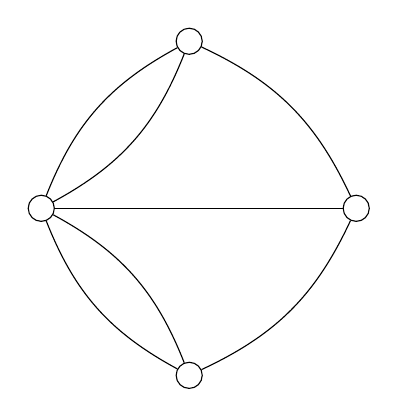
\begin{tikzpicture}[node distance = 3cm]
    \node (E) [circle, draw] {};
    \node (N) [above left of=E, circle, draw] {};
    \node (S) [below left of=E, circle, draw] {};
    \node (W) [left of=E, node distance=4cm, circle, draw] {};

    \path [-] (E) edge [bend right=20] (N)
              (E) edge [bend left=20] (S)
              (E) edge (W)
              (W) edge [bend left = 20] (N)
              (W) edge [bend right = 20] (N)
              (W) edge [bend left = 20] (S)
              (W) edge [bend right = 20] (S);
\end{tikzpicture}
\end{figure}

La domanda \`e: dato un grafo, esiste un cammino che attraverso ogni arco esattamente una volta? Un cammino in un grafo \`e una serie di vertici e archi, $v_0 e_1 v_1 e_2 x_2 \dots$, dove $e_i$ \`e l'arco che collega i vertici $x_{i - 1}$ e $x_{i}$.

Il problema del cammino per K\"{o}nigsberg \`e che alcuni vertici hanno un grado dispari.

\begin{defn}[Cammino Euleriano]
Un cammino euleriano \`e un cammino che inizia e finisce dallo stesso vertice e usa ogni arco esattamente una volta.
\end{defn}

Quel che abbiamo appena osservato \`e che se un grafo ha un nodo v con grado dispari, non esiste un cammino Euleriano. Quindi condizione necessaria affinch\'e esista un cammino Euleriano \`e che il grafo abbia tutti vertici con grado pari. \`E anche condizione sufficiente? No, il grafo deve anche essere \emph{connesso}. Le due condizioni, assieme, sono sufficienti.

\begin{figure}
\centering
\caption{Grafo non connesso, ma in cui ogni nodo ha grado pari}
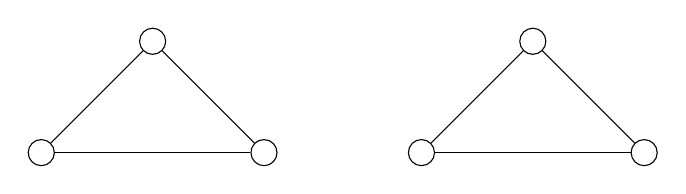
\begin{tikzpicture}[node distance=2cm]
    \node (1) [circle, draw] {};
    \node (2) [circle, draw, below left of=1] {};
    \node (3) [circle, draw, below right of=1] {};
    \node (4) [circle, draw, right of=3] {};
    \node (5) [circle, draw, above right of=4] {};
    \node (6) [circle, draw, below right of=5] {};

    \path[-] (1) edge (2)
             (2) edge (3)
             (1) edge (3)
             (4) edge (5)
             (4) edge (6)
             (5) edge (6);
\end{tikzpicture}
\end{figure}

\begin{theorem}
Sia $G$ un grafo connesso, $G$ contiene un cammino Euleriano $\iff$ ogni vertice ha grado pari. Esiste inoltre un algoritmo per trovare tale cammino.
\end{theorem}

Ci sono due aspetti da approfondire: il concetto di ``connessione'', e gli algoritmi sui grafi.

Partiamo dagli algoritmi: bisogna chiedersi prima di tutto come viene rappresentato il grafo per il computer. Ci sono principalmente due modi per rappresentarlo:
\begin{description}
    \item[Matrice di adiacenza] La matrice di adiacenza $M$ ha $n$ righe e $n$ colonne, con $\abs{V} = n$. $m_{i,j}$ \`e 1 se $v_i \adj v_j$ (i vertici $v_i$ e $v_j$ sono adiacenti), 0 se non sono adiacenti.
    \begin{figure}[h]
    \centering
    \caption{\label{fig:matrice_grafo_indiretto}Grafo indiretto}
    \begin{tikzpicture}[node distance=3cm]
        \node (1) [circle, draw] {1};
        \node (2) [circle, draw, below left of=1] {2};
        \node (4) [circle, draw, below right of=1] {4};
        \node (3) [circle, draw, below right of=2] {3};

        \path [-] (1) edge (2)
                  (1) edge (3)
                  (1) edge (4)
                  (2) edge (3)
                  (3) edge (4);
    \end{tikzpicture}
    \end{figure}
    \[
    \begin{pmatrix}
    0 & 1 & 1 & 1 \\
    1 & 0 & 1 & 0 \\
    1 & 1 & 0 & 1 \\
    1 & 0 & 1 & 0
    \end{pmatrix}
    \]
    In questo caso il grafo non \`e diretto, ed \`e quello in figura \ref{fig:matrice_grafo_indiretto}. Se invece il grafo \`e diretto, come quello in figura \ref{fig:matrice_grafo_diretto}:
    \begin{figure}[h]
    \centering
    \caption{\label{fig:matrice_grafo_diretto}Grafo diretto}
    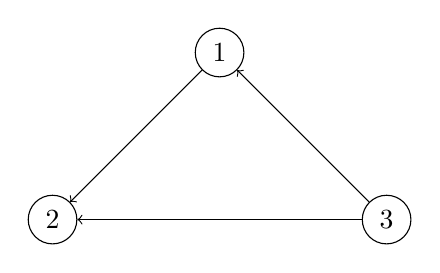
\begin{tikzpicture}[node distance=3cm]
        \node (1) [circle, draw] {1};
        \node (2) [circle, draw, below left of=1] {2};
        \node (3) [circle, draw, below right of=1] {3};

        \path [->] (1) edge (2)
                   (3) edge (1)
                   (3) edge (2);
    \end{tikzpicture}
    \end{figure}
    \[
    \begin{pmatrix}
    0 & 0 & 1 \\
    1 & 0 & 1 \\
    0 & 0 & 0
    \end{pmatrix}
    \]
    Lo spazio occupato \`e $O(n^2)$. Per vedere se due vertici $v_i$ e $v_j$ sono adiacenti, il tempo \`e costante ($O(1)$). Ma grafi con certe caratteristiche sprecare dello spazio, che si pu\`o risparmiare sapendo in partenza che il grafo ha meno archi di $n^2$.
    \item[Lista delle adiacenze] Ho una lista dei vertici, e a ogni vertice associo una lista delle adiacenze. La lista di adiacenze del grafo in figura \ref{fig:matrice_grafo_indiretto} \`e:
    \begin{align*}
    v_1 &\to [2, 3, 4] \\
    v_2 &\to [1, 3] \\
    v_3 &\to [1, 2, 4] \\
    v_4 &\to [1, 3]
    \end{align*}
    Se ci sono $m$ archi, lo spazio occupato \`e $O(n+m)$. Se voglio sapere se due vertici $v_i$ e $v_j$ sono adiacenti, il tempo \`e $O(n)$, a meno di ottimizzazioni (come ordinare le liste delle adiacenze e usare una ricerca binaria).
\end{description}

Pensiamo subito a un algoritmo. L'algoritmo deve prendere in input un grafo $G$, in cui ogni vertice ha grado almeno 2. In output l'algoritmo deve dare un ciclo in $G$. Si pu\`o dimostrare che ogni grafo in cui i vertici hanno grado almeno 2, esiste un ciclo, ma non lo faremo. Un ciclo \`e un cammino che parte e torna nello stesso vertice, percorrendo ogni arco una sola volta.

L'idea \`e di partire da un vertice qualsiasi, e di iniziare a camminare lungo gli archi incidenti nel vertice appena visto. Si potr\`a sempre continuare il cammino, perch\'e tutti i vertici hanno grado almeno due. Inoltre il grafo \`e finito: prima o poi trover\`o un vertice gi\`a visitato fra quelli adiacenti a un dato vertice, e avr\`o formato un ciclo.

\begin{algorithm}
\caption{\label{alg_ciclo_grafo_grado_due}Algoritmo per trovare un ciclo in un grafo $G$ in cui ogni nodo ha grado almeno due}
\begin{algorithmic}[1]
\Require Un grafo $G$ in cui ogni nodo $v$ ha $\deg(v) \ge 2$
\Ensure Un ciclo in $G$
\State $V \gets [x_1]$
\State $e \gets $ un arco incidente a $x_1$
\State $y \gets$ l'altro termine di $e$
\While{$y \notin V$}
    \State $V \gets V + y$
    \State $e \gets$ un arco incidente a $y$ e diverso da $e$
    \State $y \gets $ l'altro termine di $e$
\EndWhile
\State \Return $V [y, \operatorname{last}(V)]$ (ritorna il vettore $V$ da $y$ alla fine)
\end{algorithmic}
\end{algorithm}

Quanto \`e il tempo necessario per far girare l'algoritmo \ref{alg_ciclo_grafo_grado_due} quando il grafo \`e una matrice di adiacenze, e quanto quando \`e una lista di adiacenze?

Nel caso di una matrice di adiacenze, l'inizializzazione dell'algoritmo avviene in tempo costante. Il ciclo $\code{while}$ verr\`a eseguito al massimo $n$ volte. Ad ogni iterazione, per trovare un arco incidente il tempo potrebbe essere al massimo $n$. Quindi il tempo \`e $O(n \cdot n) = O(n^2)$.

Se il grafo \`e dato come una lista di adiacenze, il tempo per trovare un arco incidente a ogni iterazione \`e costante. Quindi il tempo totale sar\`a $O(n)$.

In questo caso, quindi, l'algoritmo si comporta meglio con una lista di adiacenze. In generale, quale rappresentazione sia migliore dipende dal problema.

Riprendiamo il concetto di connettivit\`a di un grafo.

\begin{defn}[Grafo connesso]
Un grafo \`e connesso se per ogni coppia di vertici $(x, y)$ esiste un cammino che parte da $x$ e finisce in $y$.
\end{defn}

Un componente di un grafo \`e un massimo sottografo connesso.

Con i grafi diretti la cosa \`e leggermente diversa. Un grafo diretto \`e fortemente connesso se per ogni coppia di vertici esiste un cammino diretto da uno all'altro e viceversa. I componenti forti sono i massimi sottografi fortemente connessi.

\`E sempre possibile partizionare i vertici di un grafo diretto per trovare una partizione in cui ogni pezzo \`e un componente forte: i singoli vertici, infatti, nel caso peggiore, sono sottografi e componenti forti.

\begin{theorem}
Sia $G$ un grafo connesso, esiste un cammino Euleriano $\iff$ ogni vertice ha grado pari.
\end{theorem}

\begin{esercizio}
Trovare un algoritmo per risolvere questo problema.
\end{esercizio}

\subsection{Problemi sui grafi}

Considerare questa matrice:
\[
\begin{matrix}
1 & 2 & 3 \\
4 & 5 & 6 \\
7 & 8 & 9
\end{matrix}
\]
Le operazioni possibili sono: spostare una riga verso destra, o una colonna verso l'alto. Vogliamo un algoritmo che, date in input due matrici di questo tipo, decide se esiste una serie di mosse che porta da una matrie all'altra (fornisce la sequenza).

Un altro esercizio: ci sono tre contenitori, uno da quattro litri, uno da sette litri, e uno da 10 litri. I primi due sono pieni. Si pu\`o versare da un contenitore all'altro fino a che o il primo \`e vuoto o il secondo \`e pieno. Dato in input una configurazione di quantit\`a di acqua in ogni contenitore, l'algoritmo deve decidere se si pu\`o arrivare a quella configurazione con le mosse dette sopra.

Cammino Hamiltoniano. L'input \`e un grafo con costi sui lati. Bisogna trovare un cammino che visita ogni vertice esattamente una volta. Non si pu\`o risolvere in maniera efficiente.

\subsection{Risolvere problemi sui grafi}

Per modellare questi problemi bisogna trattare ogni configurazione come un vertice del grafo. C'\`e un arco fra due vertici se \`e possibile passare da uno all'altro con una singola mossa.

Vediamo ora un algoritmo per risolvere questi problemi: abbiamo un grafo, un vertice iniziale e un vertice finale. Come si trova un cammino dal vertice iniziale $u$ al vertice finale $v$?

\`E pi\`u facile affrontare il problema trovando tutti i vertici raggiungibili da $u$. Si pu\`o fare in maniera \emph{greedy}. 

Ci sono diversi modi per scegliere i nuovi vertici, man mano che l'algoritmo procede:
\begin{description}
    \item[DFS] Visita in profondit\`a (Depth First Search, sezione \ref{sezione_visita_dfs})
    \item[BFS] Visita in ampiezza (Breadth First Search, sezione \ref{sezione_visita_bfs})
\end{description}

\section{Depth First Search}
\label{sezione_visita_dfs}

La visita in profondit\`a procede finch\'e pu\`o andare avanti. Quando non pu\`o pi\`u procedere, si \emph{back-tracka} il minimo possibile fino a un vertice da cui si pu\`o procedere. Bisogna mantenere un insieme di vertici gi\`a visitati, e il percorso fatto per poter tornare al vertice appena visitato. Per tutto questo, si usa uno stack. Vediamo una possibile visita $DFS$.

\begin{algorithm}
\caption{\label{visita_dfs_corr}Visita $DFS$}
\begin{algorithmic}[1]
\Require Un grafo $G$ e un vertice $u$ di $G$
\Ensure L'insieme dei vertici raggiungibili da $u$
\State $Z \gets \emptyset$ (insieme di vertici gi\`a visitati)
\State $S \gets \emptyset$ ($S$ \`e uno stack)
\State $S$.push($u$)
\State $Z \gets Z \cup u$
\While{$S \neq \emptyset$}
    \State $v \gets S$.top()
    \If{$\exists$ un vertice $x \adj v$ e $x \notin Z$} \label{lst:line:visita_dfs_corr}
        \State $Z \gets Z \cup x$
        \State $S$.push($x$)
    \Else
        \State $S$.pop()
    \EndIf
\EndWhile
\State \Return $Z$
\end{algorithmic}
\end{algorithm}

La visita $DFS$ dell'algoritmo \ref{visita_dfs_corr} trova tutti i vertici raggiungibili da $u$. Ma bisogna dimostrarne la correttezza (stiamo trovando esattamente tutti i vertici raggiungibili da $u$), e vedere il costo in termini di tempo per la ricerca. 

\begin{proof}[di completezza dell'algoritmo \ref{visita_dfs_corr}]
La completezza si dimostra per assurdo: assumiamo che ci sia un vertice $x$ raggiungibile da $u$ ma che l'algoritmo non trova.

Se \`e raggiungibile, esiste un cammino $u x_1 x_2 \dots x_l x$, che inizia da $u$ e finisce con $x$. Alcuni dei vertici saranno stati trovati dall'algoritmo. Sicuramente $u$ \`e fra questi. Individuiamo il vertice $x_{l'}$ appartenente al cammino che va da $u$ a $x$, con $l'$ a indicare il massimo valore per cui $x_{l'}$ appartiene a $Z$.

Quindi il vertice $x_{l' + 1}$ era raggiungibile nel momento in cui $x_{l'}$ \`e stato la cima dello stack $S$. La condizione alla riga \ref{lst:line:visita_dfs_corr} \`e stata vera, ma $x_{l'}$ \`e stato rimosso senza aggiungere $x_{l' + 1}$ all'insieme $Z$. Contraddizione.
\end{proof}

Quanto tempo richiede questo algoritmo? Ogni iterazione del $\code{while}$, un nodo viene o messo o tolto. Si pu\`o maggiorare tutto supponendo di inserire e togliere ciascun nodo una volta, e quindi ci sono $O(n)$ passi del ciclo.

I passi del ciclo quanto prendono? Ingenuamente, ogni passo del ciclo $\code{while}$ sembrerebbe richiedere $O(\deg (v))$ operazioni.

In realt\`a, mentre esploriamo i nodi adiacenti a un nodo $v$, ogni volta che qualche nodo adiacente a $v$ viene aggiunto a $Z$, un intero arco viene eliminato da quelli da controllare.

$Z$ pu\`o essere un vettore di booleani, e quindi essere controllabile in tempo costante.

Supponiamo di avere una lista di adiacenze. Si pu\`o cancellare un nodo dalla lista di adiacenze ogni volta che viene considerato, per ridurre il numero di controlli per trovare un nodo adiacente che non sia stato visitato.

Consideriamo $L(v)$, vettore di archi adiacenti a $v$ non ancora considerati. Mentre cerchiamo un vicino di $v$ alla riga \ref{lst:line:visita_dfs_corr} del codice, prendiamo il primo arco di $L(v)$. Se il vicino \`e un nuovo vertice,  lo aggiungiamo a $Z$ e cancelliamo l'arco da $L(v)$, altrimenti cancelliamo l'arco da $L(v)$ e prendiamo l'arco successivo.

Il numero totale di operazioni che bisogna fare per il vertice $v$ \`e costante per il grado di $v$. Quindi il tempo totale per girare \`e la somma per tutti i vertici dei gradi del vertice:
\[
O \left( \sum_{v \in V(G)} \deg (v) \right) = O (\abs{E(G)}) = O(m)
\]
$m$ indica il numero totale di archi. Infatti, la somma dei gradi di tutti i vertici (in un grafo diretto) \`e:
\[
\sum_{v \in V(G)} \deg (v) = 2 \cdot \abs{E(G)}
\]
Ogni arco viene considerato due volte.

Si pu\`o modificare l'algoritmo per farlo funzionare con grafi diretti, in modo che trovi tutti i vertici $v$ tali che esiste un cammino diretto da $u$ a $v$. Basta modificare la condizione dell'$\code{if}$ in:
\[
\exists \text{ un } x \in Z \text{ e } (v,x) \in E(G)
\]

\subsection{Alberi di visita}

L'ordine in cui vengono visitati gli archi crea un albero di visita. L'albero di visita \`e l'albero formato dagli archi ${v, x}$ dove $x$ \`e aggiunto a $Z$ mentre si considera il nodo $v$.

Un albero \`e un grafo connesso aciclico. L'albero di visita \`e aciclico perch\'e non viene mai visitato un nodo che \`e gi\`a stato visitato. Quindi ogni arco ${v,x}$ sar\`a tale che il vertice $x$ \`e ``nuovo''.

Ha qualche altra peculiarit\`a l'albero di visita: se si guardano gli archi come archi orientati, si vede che ciascun nodo ha un solo arco entrante, a parte il nodo radice, che non ne ha nessuno. Questo particolare tipo di albero \`e detto ``arborescenza''.

\begin{defn}[Arborescenza]
Un'arborescenza \`e un albero diretto dove ogni nodo ha un arco entrante, tranne la radice che non ha nessun arco entrante.
\end{defn}

La ricerca DFS si usa per trovare tutti i componenti di un grafo (indiretto). Si fissa un vertice $u$, e si cercano tutti i nodi raggiungibili. Il risultato \`e un componente. Finch\'e ci sono vertici del grafo che non appartengono a un componente, si ripete il processo per uno dei vertici, e si trova ogni volta un nuovo componente.

\begin{exmp}
Dobbiamo programmare $n$ esami in un periodo di 2 settimane. Ci sono $k$ studenti che devono sostenere gli esami. Vogliamo dividere gli esami in modo che nessuno dei $k$ studenti debba fare due esami nella stessa settimana. Possiamo assumere che nessuno studente debba fare pi\`u di 2 esami. Siccome uno studente che deve fare un solo esame non \`e rilevante al nostro problema, possiamo direttamente assumere che tutti i $k$ studenti devono fare esattamente due esami.

Per risolvere il problema, rappresentiamo ogni esame con un nodo, e tracciamo un arco fra due nodi se uno studente deve sostenere entrambi gli esami. Il problema ora \`e trovare una partizione dei nodi in due insiemi $U_1$ e $U_2$ in modo che ogni arco ha i propri termini in partizioni distinte. Alternativamente possiamo colorare i nodi del grafo con due colori in modo che nessun arco abbia i termini dello stesso colore.

Si pu\`o risolvere il problema con una visita $DFS$. Il primo nodo viene messo nell'insieme 1. Tutti i vicini vengono messi nell'insieme 2. I loro vicini, ancora, vengono messi nell'insieme 1.
\begin{enumerate}
    \item Usando una visita $DFS$ troviamo un albero di visita per il grafo.
    \item Fissiamo un vertice $r$ e mettiamo $r$ in $U_1$ (\`e simmetrico fino a questo punto).
    \item Il fatto che $r$ sia in $U_1$, forza tutti gli altri vertici a essere o in $U_1$ o in $U_2$. Ossia, una volta determinato l'insieme a cui appartiene la radice, troviamo a quale insieme appartengono tutti gli altri. Ora ogni arco ha un colore.
    \item\label{itm:last_step_colorazione} Ora bisogna controllare tutti gli altri archi, e vedere se un arco unisce due vertici che appartengono allo stesso insieme (o che sono dello stesso colore).
\end{enumerate}
Non \`e importante che il grafico sia connesso. Questo algoritmo si pu\`o applicare componente per componente per trovare le colorazioni dei vertici di ciascun componente (visto che i singoli componenti sono indipendenti gli uni dagli altri).

Se il passo numero \ref{itm:last_step_colorazione} fallisce, il grafo non si pu\`o colorare come volevamo. La colorazione ottenuta \`e l'unica possibile, a meno di invertire i due colori.

Se si vuole cambiare il problema a dividere fra gli esami in tre settimane distinte? Bisogna colorare con 3 colori distinti. Ogni studente pu\`o mettere due archi fra tre esami.

La differenza \`e nel fatto che, colorato il primo nodo, i suoi nodi adiacenti possono essere colorati in due modi distinti, e cos\`i via. Ci sono $2^{n-1}$ modi per colorare gli $n-1$ nodi diversi dalla radice. Il nostro algoritmo \`e diventato esponenziale.

Probabilmente non esiste un algoritmo polinomiale per colorare con pi\`u di 2 colori un grafo.
\end{exmp}

\begin{exmp}[Ordinamento topologico]
Una fabbrica ha diviso un processo in $n$ fasi di lavoro. Per alcune coppie $\{a,b\}$ di fasi di lavoro, \`e necessario che queste vengano compiute in un certo ordine ($(a,b)$ o $(b,a)$). Bisogna trovare un ordine delle fasi di lavoro che non abbia conflitti, ossia una sequenza $a_1 a_2 \dots a_i a_j \dots a_n$ tale per cui non esistono due indici $i < j$ tali per cui $a_j$ va completata prima di $a_i$.

Creiamo un grafo orientato con per vertici le fasi di lavoro $a_i$. Mettiamo un arco dal nodo $a$ al nodo $b$ se il nodo $a$ deve essere finito prima di $b$.

Se nel grafo \`e presente un ciclo (diretto), il problema non ha soluzione.

\begin{prop}
\label{grafo_diretto_aciclico}
Un grafo diretto senza cicli ha due vertici $u$ e $v$ tali che $u$ non ha archi entranti e $v$ non ha archi uscenti.
\end{prop}

Se il grafo \`e aciclico, grazie a questa proposizione, posso iniziare la visita proprio dal vertice che non ha archi entranti.

\begin{algorithm}
\caption{Algoritmo per l'ordinamento topologico}
\begin{algorithmic}[1]
\Require Un grafo diretto $G$ senza cicli
\Ensure Un ordinamento dei vertici che rispetta l'orientamento degli archi
\State $L \gets [\;]$ (una lista vuota)
\While{$\exists $ un vertice in $G$}
    \State $u \gets$ un vertice senza archi entranti
    \State $G \gets G \setminus \{ u \}$
    \State $L \gets L + [u]$
\EndWhile
\State \Return $L$
\end{algorithmic}
\end{algorithm}

Il ciclo $\code{while}$ richiede $n$ passi, per $n+m$ passi per trovare il vertice senza archi entranti. Quindi il tempo \`e $O(n(n+m))$.

Un ordinamento topologico \`e un ordinamento dei vertici tale per cui due vertici $v_i < v_j$ sono tali che $(v_i, v_j) \notin E(G)$.
\end{exmp}

Un grafo diretto senza cicli si chiama \emph{DAG} (Directed Aciclic Graph).

\begin{prop}
Dato un grafo $G$ in cui \`e vera una delle seguenti affermazioni:
\begin{enumerate}
    \item $\forall v \in V$ esiste un arco entrante
    \item $\forall v \in V$ esiste un arco uscente
\end{enumerate}
esiste un algoritmo efficiente in grado di trovare un ciclo.
\end{prop}

Il presupposto di questa proposizione \`e una negazione della proposizione \ref{grafo_diretto_aciclico}: un grafo \`e aciclico se esiste un vertice senza archi entranti e esiste un vertice senza archi uscenti, quindi un grafo \`e ciclico se tutti i vertici hanno un arco entrante o tutti i vertici hanno un arco uscente. 

\begin{proof}[della proposizione \ref{grafo_diretto_aciclico}]
Facciamo la dimostrazione con un algoritmo. Per trovare un ciclo basta usare una DFS.

\begin{algorithm}
\caption{Algoritmo per trovare un ciclo}
\begin{algorithmic}[1]
\Require Un grafo $G$ che rispetta i presupposti della proposizione \ref{grafo_diretto_aciclico}
\Ensure Un ciclo $L$ in $G$
\State $L \gets [x]$, con $x \in G$ (una lista)
\While{$L$.last() ha un vertice adiacente $u \notin L$}
    \State $v \gets L$.last()
    \State $u \gets $ un vertice tale per cui $v \adj u$
    \If{$u \notin L$}
        \State $L$.append($u$)
    \EndIf
\EndWhile
\State \Return $L[u, v]$
\end{algorithmic}
\end{algorithm}

Un grafo \`e diretto e aciclico $\iff$ esiste un ordinamento topologico.

Per capire quanto tempo impiega l'algoritmo a girare, aggiungiamo due contatori nel DFS. $t(v)$ \`e il numero di nodi visitati prima di $v$ (incluso $v$), ossia il numero di nodi visitati quando incontriamo $v$ per la prima volta, mentre $T(v)$ \`e il numero di nodi visitati dopo $v$ quando l'algoritmo termina, ossia il numero di nodi visitati l'ultima volta che visitiamo $v$.
\end{proof}

\begin{figure}
\centering
\caption{\label{fig:visita_dfs}Esempio di visita DFS su un grafo}
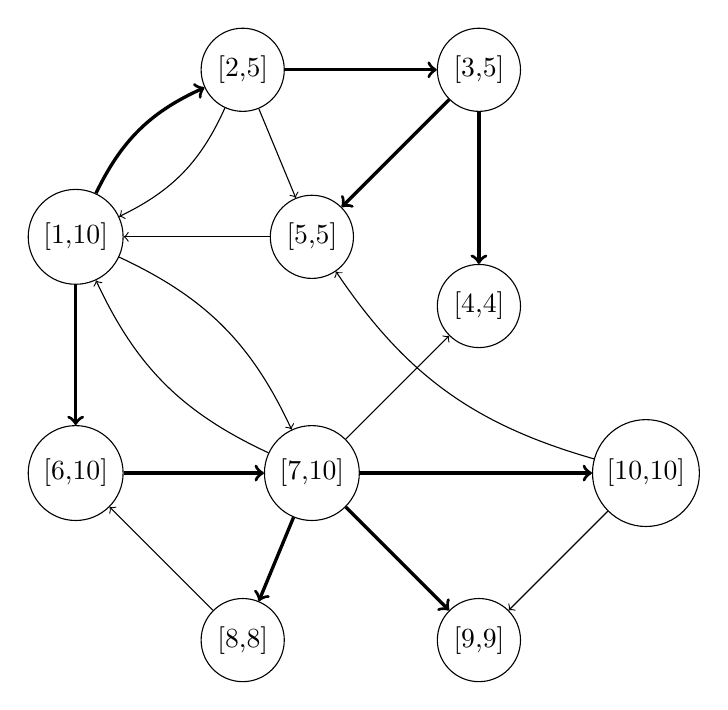
\begin{tikzpicture}[node distance=3cm]
    \node (1) [circle, draw] {[1,10]};
    \node (2) [circle, draw, above right of=1] {[2,5]};
    \node (3) [circle, draw, right of=2] {[3,5]};
    \node (4) [circle, draw, below of=3] {[4,4]};
    \node (5) [circle, draw, below left of=3] {[5,5]};
    \node (6) [circle, draw, below of=1] {[6,10]};
    \node (7) [circle, draw, right of=6] {[7,10]};
    \node (8) [circle, draw, below right of=6] {[8,8]};
    \node (9) [circle, draw, right of=8] {[9,9]};
    \node (10) [circle, draw, above right of=9] {[10,10]};

    \path[->] (2) edge [bend left=20] (1)
              (2) edge (5)
              (5) edge (1)
              (1) edge [bend left=20] (7)
              (7) edge [bend left=20] (1)
              (7) edge (4)
              (8) edge (6)
              (10) edge (9)
              (10) edge [bend left=20] (5);

    \path[->, very thick] (1) edge [bend left=20] (2)
              (2) edge (3)
              (3) edge (4)
              (3) edge (5)
              (1) edge (6)
              (6) edge (7)
              (7) edge (8)
              (7) edge (9)
              (7) edge (10);

\end{tikzpicture}
\end{figure}

$\forall u, v$ ci sono le due coppie di intervalli $[t(u), T(u)]$ e $[t(v), T(v)]$. I casi possibili sono tre:
\begin{enumerate}
    \item $[t(u), T(u)] \subseteq [t(v), T(v)]$
    \item $[t(u), T(u)] \supseteq [t(v), T(v)]$
    \item $[t(u), T(u)] \cap [t(v), T(v)] = \emptyset$
\end{enumerate}

Se $(u,v)$ \`e un arco, ci sono tre casi:
\begin{enumerate}
    \item $(u,v)$ ``passa dietro'' nella visita
    \item $(u,v)$ ``passa avanti'' nella visita
    \item $(u,v)$ \`e un arco di attraversamento. Deve essere che $t(u) > t(v)$.
\end{enumerate}

\begin{prop}
Sia $G$ un grafo diretto, $G$ \`e aciclico $\iff$ l'albero di visita DFS non ammette archi che ``passano dietro''.
\end{prop}

Siccome l'albero contiene sempre un cammino diretto da $u$ a tutti i vertici $v$ tali che si finisce con $v$ prima che si finisce con $u$, allora $(v,u)$ completa sempre un ciclo se $[t(u), T(u)] \supseteq [t(v), T(v)]$. 

Se $(u,v)$ \`e un arco \emph{non} nell'albero di visita, ci sono tre casi:
\begin{enumerate}
    \item $[t(u), T(u)] \cap [t(v), T(v)] = \emptyset \implies (u,v)$ \`e un arco di attraversamento. Un esempio nel grafo in figura  \ref{fig:visita_dfs} \`e l'arco (10,5). In questo caso deve essere che $t(u) > T(v)$. Quindi vediamo il nodo $u$ per la prima volta dopo aver visto il nodo $v$ per l'ultima volta.
    \item $[t(u), T(u)] \subseteq [t(v), T(v)]$, allora l'arco $(u,v)$ \`e un arco che ``torna indietro'', come l'arco (5,1) nel grafico in figura \ref{fig:visita_dfs}.
    \item $[t(u), T(u)] \supseteq [t(v), T(v)]$, allora l'arco $(u,v)$ \`e un arco ``in avanti'', come l'arco (1,7).
\end{enumerate}

Fino ad ora abbiamo visto un grafo diretto. Se il grafo indiretto, archi ``avanti'' e ``indietro'' coincidono. Inoltre, sempre se il grafo non \`e diretto, non esistono archi di attraversamento.

Gli archi di attraversamento portano da un nodo a un altro nodo contenuto su un sottoalbero diverso dal sottoalbero attuale dell'albero di visita.

Se un grafo non \`e diretto, e se $T$ \`e l'albero di visita di un algoritmo DFS, la presenza di archi ``all'indietro'' implica la presenza di un ciclo.

Per ogni coppia di vertici $(x,y)$ esiste un cammino che parte da $x$ e arriva a $y$ nell'albero di visita $T$. Se esiste un arco ``all'indietro'' $(x,y)$ che non appartiene all'albero di visita $T$, allora esiste un ciclo nel grafo $G$.

Quindi, se esiste un ciclo nel grafo $G$, allora $T$ ha un arco ``all'indietro''. Vale anche che, se $T$ non ha archi all'indietro, $G$ non ha cicli. Infatti, $T$ pu\`o avere solo archi all'indietro, essendo $G$ un grafo indiretto, e se non ne ha non pu\`o avere archi (l'albero di visita \`e un albero, quindi aciclico).

\begin{prop}
Sia $G$ un grafo indiretto, esiste un ciclo in $G \iff $ esiste un arco all'indietro nell'albero di visita DFS di $G$.
\end{prop}

Con i grafi diretti, non si pu\`o pi\`u dire che fra ogni coppia $(x,y)$ esiste un cammino da uno all'altro.

Prendiamo un generico arco $(y,x)$. Se $(y,x)$ \`e un arco all'indietro, come l'arco $(5,1)$ nella figura \ref{fig:visita_dfs}, allora esiste un ciclo diretto in $G$.

\begin{oss}
Tutti i vertici $y$ tali che $t(x) \le t(y) \le T(x)$ sono raggiungibili nell'albero di visita con un cammino diretto che parte da $x$ e arriva a $y$.
\end{oss}
\`E un po' una banalit\`a.

Se c'\`e un arco all'indietro, allora $[t(y), T(y)] \subseteq [t(x), T(x)]$, e quindi l'arco $(y,x)$ deve completare un ciclo diretto.

Dobbiamo far vedere anche che se esiste un arco all'indietro, deve esistere anche un ciclo nel grafo.

\begin{figure}
\centering
\begin{tikzpicture}
    \node (c0) [circle, draw, label=$c_0$] {};
    \node (c1) [circle, draw, label=$c_1$, below right = of c0] {};
    \node (c2) [circle, draw, label=$c_2$, below left = of c1] {};
    \node (c3) [circle, draw, label=$c_3$, left = of c2] {};
    \node (cn) [above left = of c3] {$\dots$};
    \node (ck) [circle, draw, label=$c_k$, above right = of cn] {};

    \path [->] (c0) edge (c1)
               (c1) edge (c2)
               (c2) edge (c3)
               (c3) edge (cn)
               (cn) edge (ck)
               (ck) edge (c0);
\end{tikzpicture}
\end{figure}

Prima di tutto, $t(c_0) \le t(c_i) \forall i \ge 1$. Ci sono archi che appartengono all'albero, ma non tutti sono archi all'indietro.

\begin{claim}
Per tutti gli indici $i \ge 1$, deve essere vero che $c_i$ viene completato prima della chiusira di $c_0$. Ossia, $T(c_i) \le T(c_0)$.
\end{claim}

\begin{proof}
Assumiamo per assurdo che esiste un $j$ tale che $T(c_j) \ge T(c_0)$, e sia $j$ proprio il valore minore per cui questo vale, allora vale che $T(c_{j-1}) \le T(c_0) \le T(c_j)$. Quindi $c_{j-1}$ viene visitato per l'ultima volta prima di aver visitato per l'ultima volta $c_j$. 

% grafico tempo con apertura e chiusura c_0 e c_{j-1}

Non pu\`o essere che $[t(c_j), T(c_{j})] \cap [t(c_{j-1}), T(c_{j-1})] \neq \emptyset$. Quindi o sono completamente disgiunti, ma $t(c_j)$ non pu\`o venire dopo $T(c_0)$, o sono contenuti uno nell'altro. Deve essere necessariamente che $[t(c_j), T(c_{j})] \supseteq [t(c_{j-1}), T(c_{j-1})]$, ma deve essere anche che $[t(c_j), T(c_{j})] \supseteq [t(c_{0}), T(c_{0})]$, poich\'e $T(c_{j-1})$ appartiene a entrambi. Siamo arrivati all'assurdo: non pu\`o essere che $t(c_j) \le t(c_0)$, perch\'e per ipotesi siamo partiti da $c_0$.
\end{proof}

Non abbiamo finito. Stiamo cercando un arco all'indietro. L'arco all'indietro \`e quello fra $(c_k, c_0)$. Abbiamo dimostrato che $T(c_k) \le T(c_0)$, e sappiamo inoltre che $t(c_0) \le t(c_k)$. Quindi $[t(c_k), T(c_k)] \subseteq [t(c_0), T(c_0)]$, e quindi c'\`e un arco all'indietro fra $(c_k, c_0)$.

\begin{prop}
Se esiste un ciclo diretto in un grafo $G$ diretto, esiste anche un arco all'indietro in un albero di visita DFS, e se esiste un arco all'indietro in un albero di visita DFS del grafo $G$, allora esiste un ciclo diretto nel grafo.
\end{prop}

C'\`e un modo semplice per memorizzare l'albero di visita: basta associare ad ogni vertice il vertice che l'ha scoperto. Quindi, se $u$ scopre il vertice $v$, per ricostruire l'albero basta memorizzare l'informazione che $u$ \`e il \emph{padre} di $v$. Per definizione il nodo radice non ha un padre, e questo si rappresenta con la convenzione $P(u) = u$, ossia il padre del nodo radice \`e il nodo stesso.

Per memorizzare l'albero di visita usiamo il vettore $P$ dei padri dei nodi. 

\begin{esercizio}
Dato in input il vettore $P$ dei padri, progettare un algoritmo che ricostruisce l'albero di visita come una lista di adiacenze.
\end{esercizio}

Si pu\`o usare il vettore per memorizzare se un nodo \`e o meno ancora dentro lo stack (ossia, deve essere analizzato). Se presumiamo che i vertici sono numerati con un intero da 1 a $n$, la prima volta che visitiamo un vertice $v$ (da un vertice $u$), settiamo $P[v] = -u$, e quando chiudiamo $u$ settiamo $P[v] = - P[v]$.

Se durante una visita DFS trovo un arco $(v,w)$, per sapere se l'arco \`e un arco che porta a un nodo gi\`a visitato devo controllare se $P[w] \neq 0$. Inoltre, $P[w] < 0$ se e solo se $(v,w)$ \`e un arco all'indietro. Quindi ora possiamo scrivere un algoritmo per trovare un ciclo in un grafo diretto tramite DFS.

\begin{algorithm}
\caption{Visita DFS per trovare un ciclo}
\begin{algorithmic}[1]
\State $P \gets$ vettore dei padri dei nodi inizializzato a 0
\Function{DFS\_CYCLE}{$G$ grafo, $v$ nodo, $u$ nodo, $P$ vettore}
    \State $P[v] \gets -u$
    \ForAll{$w$ adiacente a $v$}
        \If{$P[w] = 0$}
            \State $z \gets $ \Call{DFS\_CYCLE}{$G$, $w$, $v$, $P$}
            \If{$z \neq 0$}
                \State $P[v] \gets - P[v]$
                \State \Return $z$
            \EndIf
        \ElsIf{$P[w] < 0 \land (G$ diretto $\lor w \neq v)$}
            \State $P[w] = 0$
            \State $P[v] = u$
            \State \Return $v$
        \EndIf
        \State $P[v] = u$
        \State \Return $0$
    \EndFor
\EndFunction
\State $w \gets$ \Call{DFS\_CYCLE}{$G$, $u$, $u$, $P$}
\State $L \gets$ lista vuota
\While{$w > 0$}
    \State $L$.append($w$)
    \State $w \gets P[w]$
\EndWhile
\State \Return $L$
\end{algorithmic}
\end{algorithm}

$v$ \`e la radice, $u$ \`e il padre della radice. La funzione ritorna 0 se non trova nessun ciclo, un numero diverso da 0 se trova un ciclo.

Sia $G$ un grafo diretto senza cicli, vogliamo trovare un ordine topologico $x_1, x_2, \dots x_n$ in cui tutti gli archi sono $(x_i, x_j)$ con $x_i < x_j$. Una buona scelta per l'ultimo vertice dell'ordinamento \`e un nodo che non ha archi uscenti (che ci deve essere, lo sappiamo). Con un DFS ordiniamo i vertici partendo dall'ultimo, quello che viene ``chiuso'' per primo.

\subsection{Grafo di una citt\`a}

\begin{esercizio}
In un grafo diretto, i nodi rappresentano le intersezioni fra strade, e gli archi corrispondono alle strade. Un arco $f$ si dice \emph{arco critico} se $G - f$ non \`e pi\`u connesso. Il problema \`e determinare se un grafo ha un arco critico o meno.
\end{esercizio}

Si cancella l'arco $(u,v)$ e si controlla se si pu\`o ancora raggiungere $u$ da $v$. La complessit\`a \`e $O(m \cdot (n + m))$: un controllo DFS per tutti gli m archi.

Lo stesso algoritmo serve a trovare tutti i ponti in un grafo non diretto. Per\`o l'algoritmo \`e inefficiente. Proviamo a modificare il DFS per renderlo $O(n + m)$, nel caso in cui il grafo sia indiretto.

Fissiamo un vertice $v$ da cui costruire l'albero di visita DFS (con radice in $v$). Gli archi che non appartengono all'albero \emph{sicuramente} non sono ponti: anche eliminandoli si pu\`o sempre raggiungere tutto il grafo. Quindi se un arco \`e un ponte, l'arco appartiene a $E(T)$ (gli archi dell'albero di visita DFS). Ora il tempo \`e $O(n \cdot (n + m))$, controllando solo gli archi nell'albero (che sono $n$).

Consideriamo ora un arco $f = (u,w)$ all'interno dell'albero di visita, e chiamiamo $T(w)$ l'insieme di vertici che vengono dopo $w$ (nel sottoalbero con radice in $w$). Se esiste un arco all'indietro in $T(w)$ a un antenato di $u$ (o a $u$), allora $f$ non \`e un ponte. \`E un se e solo se: se esiste un ponte, allora esiste un arco all'indietro da $T(w)$ a un antenato di $u$ (o a $u$). O con altre parole, se $f$ non \`e un ponte esiste un cammino che porta da $u$ a $T(w)$, e quindi deve esserci un arco all'indietro da $T(w)$ a $u$.

Conclusione: un arco $f = (u,w)$ nell'albero DFS \`e un ponte $\iff$ non esiste un arco all'indietro con un termine dentro $V(T(w))$ e l'altro termine uguale a $u$ o un antenato di $u$.

\begin{algorithm}
\caption{Visita DFS per trovare un ponte}
\begin{algorithmic}[1]
\State $tt \gets$ array del momento della prima visita, inizializzato a 0
\State $c \gets$ contatore inizializzato a 0
\State $p \gets$ lista dei ponti, inizializzata a 0
\Function{DFS\_PONTE}{$G$ grafo, $u$ nodo, $z$ nodo, $tt$ array, $c$ intero, $p$ lista}
    \State $c \gets c + 1$
    \State $tt[u] \gets c$
    \State $back \gets c $
    \ForAll{$v \adj u$}
        \If{$tt[v] = 0$} (non \`e stato visitato)
            \State $b \gets$ \Call{DFS\_PONTE}{$G,v,u,tt,c,p$}
            \If{$b > tt[u]$}
                \State $p$.append($\{u,v\}$)
            \EndIf
            \State $back \gets \min(back, b)$
        \ElsIf{$v \neq z$}
            \State $back \gets \min(back, tt[v])$
        \EndIf
    \EndFor
    \State \Return $back$
\EndFunction
\end{algorithmic}
\end{algorithm}

\begin{defn}[Vertici di articolazione]
Un vertice di articolazione \`e un vertice $v$ tale per cui $G - v$ non \`e connesso.
\end{defn}
$G - v$ \`e il grafo senza il vertice $v$ e senza tutti gli archi incidenti a $v$.

Se $\{ u, v \}$ \`e un ponte incidente a $v$, $v$ \`e un vertice di articolazione $\iff \deg(v) = 2$.

Non vale l'inverso: se $v$ \`e un vertice di articolazione, gli archi incidenti a $v$ non sono necessariamente ponti. O anche: se esiste un vertice di articolazione, non necessariamente esiste un ponte.

Ora vogliamo usare un metodo simile a quello appena visto per trovare tutti i vertici di articolazione.

Sia $T$ l'albero DFS con radice $u$. Se $u$ ha un solo figlio, $u$ non \`e un vertice di articolazione, perch\'e qualunque cammino dentro l'albero fra due vertici non passer\`a mai per $u$, poich\'e dovrebbe passare due volte sullo stesso arco. Quindi, siccome esiste un cammino dal nodo $x$ al nodo $y$ in $T - u$, $T - u$ \`e connesso.

Se $u$ ha pi\`u di un figlio, perch\'e non sia un nodo di articolazione dovrebbe esistere un arco di attraversamento fra i sottoalberi individuati dai figli. Ma in un grafo indiretto tutti gli archi sono archi all'indietro, e mai archi di attraversamento, quindi $u$ \`e un nodo di articolazione.

Quindi, in conclusione, $u$ \`e un vertice di articolazione $\iff \deg_T (u) \ge 2$. Il tempo per trovare se un vertice \`e un nodo di articolazione \`e $O(n + m)$. Per trovare tutti i vertici di articolazione bisogna di nuovo usare una DFS modificata, per ottenere di nuovo un tempo $O(n+m)$.

\begin{algorithm}
\caption{Algoritmo per trovare i vertici di articolazione}
\begin{algorithmic}[1]
\State $tt \gets$ vettore del momento della prima visita, inizializzato a 0
\State $c \gets 0$
\State $A \gets$ insieme vuoto di vertici di articolazione
\Function{DFS\_ART}{$G$ grafo, $v$ nodo, $tt$, $c$, $A$}
    \State $c \gets c + 1$
    \State $tt[v] \gets c$
    \State $children \gets 0$
    \State $back \gets c$
    \ForAll{$w \adj v$}
        \If{$tt[w] = 0$}
            \State $children \gets children + 1$
            \State $b \gets$ \Call{DFS\_ART}{$G, w, tt, c, A$}
            \If{$tt[v] > 1 \land b \ge tt[v]$} (non vale per la radice)
                \State $A$.add($v$)
            \EndIf
            \State $back \gets \min(back, b)$
        \Else
            \State $back \gets \min(back, tt[w])$
        \EndIf
    \EndFor
    \If{$tt[v] = 1 \land children \ge 2$}
        \State $A$.add($v$)
    \EndIf
    \State \Return $back$
\EndFunction
\end{algorithmic}
\end{algorithm}

\begin{defn}[Nodo critico]
Dati due nodi $a$ e $b$, un nodo $c$ diverso da $a$ e da $b$ si dice critico per $a$ e $b$ se ogni cammino da $a$ a $b$ contiene $c$.
\end{defn}

Per controllare se un dato nodo $x$ \`e un nodo critico per un paio di vertici $a, b$ basta controllare se esiste un cammino da $a$ a $b$ in $G - x$.

Per avere tutti i nodi critici dati due nodi $a$ e $b$, si potrebbe controllare ogni altro vertice, ma il tempo sarebbe $O(n \cdot (n + m))$.

\begin{oss}
Dati due vertici $a$ e $b$ e un vertice $c$ critico per $a$ e $b$, $c$ \`e un vertice di articolazione, perch\'e $a$ appartiene a un componente di $G - c$ e $b$ appartiene a un componente di $G - x$, e questi componenti devono essere distinti perch\'e non c'\`e nessun cammino da $a$ a $b$.
\end{oss}

Non vale l'inverso: un vertice di articolazione non \`e un nodo critico per due vertici $a$ e $b$.

Abbiamo un algoritmo per trovare tutti i vertici di articolazione in tempo $O(n + m)$. Possiamo notare che, dato un qualsiasi cammino $P$ da $a$ a $b$, tutti i vertici critici per $a$ e $b$ (se ci sono) devono essere in questo cammino.

Un grafo \`e biconnesso se per ogni vertice $x$, $G - x$ \`e connesso. Un componente biconnesso \`e un sottografo massimale che \`e biconnesso. Un ciclo \`e sempre biconnesso. Dobbiamo modificare il DFS visto l'ultima volta per trovare tutti i componenti biconnessi. Un vertice in comune fra componenti biconnessi \`e sempre un vertice di articolazione. I nodi critici sono i vertici di articolazione fra i componenti biconnessi contenenti $a$ e $b$.

\subsection{Forte connettivit\`a in grafi diretti}

Per determinare se un grafo diretto \`e fortemente connesso, potrei $\forall u \in V (G)$ fare un $\operatorname{DFS}(G,u)$ e se esiste un vertice $v$ non connesso a $u$, ritornare falso, altrimenti ritornare vero. Ma il tempo \`e esagerato: $O(n \cdot (n + m))$.

Il grafo trasposto $G^T$ \`e il grafo con l'orientamento di tutti gli archi invertito. Per determinare se per tutti i vertici $v$ esiste un cammino da $v$ a $u$, basta fare un $\operatorname{DFS}(G^T, u)$. Quindi l'algoritmo \`e:

\begin{algorithm}
\caption{Test per la forte connettivit\`a in un grafo diretto}
\begin{algorithmic}[1]
    \State fisso un vertice $u$
    \State $T_1 \gets$ l'albero di ricerca del $\operatorname{DFS}(G, u)$
    \State $T_2 \gets$ l'albero di ricerca del $\operatorname{DFS}(G^T, u)$
    \If{$V(T_1) = V(T_2) = V(G)$}
        \State \Return TRUE
    \Else
        \State \Return FALSE
    \EndIf
\end{algorithmic}
\end{algorithm}

\begin{prop}
Sia $G$ un grafo diretto e sia $u \in V(G)$, $T_1$ l'albero di ricerca di $\operatorname{DFS}(G, u)$ e $T_2$ l'albero di ricerca $\operatorname{DFS}(G^T, u)$, $G$ \`e fortemente connesso $\iff V(T_1) = V(T_2) = V(G)$.
\end{prop}

Infatti, dati comunque due vertici $x, y \in V(G)$, esiste un cammino da $x$ a $u$ e un cammino da $u$ a $y$, e quindi esiste una ``passeggiata'' da $x$ a $y$. (Si chiama passeggiata, e non cammino, perch\'e pu\`o essere un cammino che passa pi\`u volte sugli stessi nodi)

Se volessimo trovare i componenti fortemente connessi di un grafo? Abbiamo visto che i grafi biconnessi possono intersecarsi, ma i componenti fortemente connessi non possono avere intersezione non vuota.

\begin{defn}[Componente fortemente connesso]
Un componente fortemente connesso di un grafo $G$ \`e un sottografo massimale fortemente connesso.
\end{defn}

Siano $U_1$ e $U_2$ insiemi di vertici di componenti fortemente connessi, allora $U_1 \cap U_2 = \emptyset$, altrimenti per $x, y \in U_1 \cup U_2$ esiste un cammino da $x$ a un vertice appartenente a $U_1 \cap U_2$, e un cammino da questo vertice a $y$, e quindi esiste un cammino da $x$ a $y$.

Fissiamo un nodo $u$ e cerchiamo il componente che contiene questo nodo.
\begin{align*}
T_1 &= \operatorname{DFS}(G, u) \\
T_2 &= \operatorname{DFS}(G^T, u)
\end{align*}
Il componente fortemente connesso contenente $u$, per gli stessi motivi di prima, \`e $V(T_1) \cap V(T_2)$. Infatti ciascuna coppia di vertici in $V(T_1) \cap V(T_2)$ \`e fortemente connessa, e ciascun nodo all'esterno dell'intersezione non \`e fortemente connesso. Il tempo per trovare questo componente fortemente connesso per\`o \`e $O(n \cdot (n + m))$.

Diamo qualche definizione.

\begin{defn}
Il sottografo indotto su un insieme di vertici $X$ \`e il sottografo con vertici in $X$ e tutti gli archi di $G$ con entrambi i termini dentro $X$. Si indica con $G[X]$.
\end{defn}

Siano $G[U_1]$ e $G[U_2]$ due sottografi indotti fortemente connessi, con un arco da $U_1$ a $U_2$ e un arco da $U_2$ a $U_1$, allora $G[U_1 \cup U_2]$ \`e un sottografo indotto fortemente connesso.

\begin{defn}
Per contrarre un insieme di vertici $X$ in un grafo, tolgo $X$ e aggiungo un vertice nuovo $V_X$ e per ogni arco $(z,y)$ o $(y,z)$ con $z \in X$ e $y \notin X$ aggiungo un arco da $V_X$ a $y$ o da $y$ a $V_X$. Il grafo contratto si scrive $G / X$.
\end{defn}

\begin{figure}
\centering
\caption{Grafo contratto}
\begin{tikzpicture}[node distance=1.5cm]
    \node (A1) [circle, draw] {}; 
    \node (A2) [circle, draw, above right = of A1] {}; 
    \node (A3) [circle, draw, below right = of A1] {}; 
    \node (A4) [circle, draw, below right = of A2] {};

    \node (A5) [circle, draw, above right = of A2] {}; 
    \node (A9) [circle, draw, below right = of A3] {}; 

    \node (A6) [circle, draw, right = of A5] {}; 
    \node (A8) [circle, draw, right = of A9] {}; 
    \node (A7) [circle, draw, right = 3.5cm of A4] {}; 

    \path[->]   (A1) edge [bend left=20] (A2)
                (A2) edge [bend left=20] (A4)
                (A3) edge [bend left=20] (A1)
                (A4) edge [bend left=20] (A3)
                (A2) edge (A5)
                (A5) edge (A6)
                (A6) edge (A7)
                (A7) edge (A8)
                (A8) edge (A9)
                (A9) edge (A3);

    \node (B1) [circle, draw, right = of A7] {$V_X$}; 

    \node (B5) [circle, draw, above right = of B1] {}; 
    \node (B9) [circle, draw, below right = of B1] {}; 

    \node (B6) [circle, draw, right = of B5] {}; 
    \node (B8) [circle, draw, right = of B9] {}; 
    \node (B7) [circle, draw, below right = of B6] {}; 

    \path[->]   (B1) edge (B5)
                (B5) edge (B6)
                (B6) edge (B7)
                (B7) edge (B8)
                (B8) edge (B9)
                (B9) edge (B1);
\end{tikzpicture}
\end{figure}

\begin{prop}
Sia $U$ un insieme di vertici tali per cui il sottografo indotto $G[U]$ \`e fortemente connesso, se $G / U$ \`e fortemente connesso, allora anche $G$ \`e fortemente connesso.
\end{prop}

Creiamo un nuovo algoritmo: in input prende un grafo $G$, e in output d\`a una lista $\{ U_1, U_2, \ldots, U_l \}$ dei componenti fortemente connessi.

\begin{algorithm}
\caption{Come \emph{non} trovare i componenti fortemente connessi}
\begin{algorithmic}[1]
\Function{Fort}{$G$ grafo}
    \State trova un ciclo $C$ in $G$
    \If{non esiste un ciclo $C$}
        \State \Return $(\{ v \} : v \in V(G))$
    \EndIf
    \State $\{ U_1, \ldots, U_l \} \gets$ \Call{Fort}{G / C}
    \ForAll{$U_i \in \{U_1, \ldots, U_l \}$}
        \If{$V_C \in U_i$}
            \State $U_i' \gets (U_i - V_C) \cup V(C)$
        \Else
            \State $U_i' \gets U_i$
        \EndIf
    \EndFor
    \State \Return $\{ U_1', \ldots, U_l' \}$
\EndFunction
\end{algorithmic}
\end{algorithm}

La ricorsione pu\`o esser fatta al massimo $O(n)$ volte, poich\'e $G$ decresce ad ogni passo. Ad ogni passo, ci vuole $O(n + m)$ per trovare un ciclo. Quindi il tempo totale pu\`o essere maggiorato con $O(n \cdot (n + m))$. Che non \`e un tempo ottimale.

\section{Componenti fortemente connessi}

\begin{defn}[C-radice]
Una C-radice \`e il primo nodo trovato in un componente fortemente connesso durante un dato DFS.
\end{defn}

\begin{prop}
Un nodo $u$ non \`e una C-radice $\iff$ nella chiamata ricorsiva del $DFS$ con radice $u$ viene attraversato un arco $(v,w)$ tale che il nodo $w$ \`e gi\`a stato visitato (quindi $t[w] < t[u]$) e il componente di $w$ non \`e ancora stato determinato.
\end{prop}

\begin{proof}
Se $u$ non \`e una C-radice, la C-radice per il componente fortemente connesso contenente $u$ si trova \emph{prima} di $u$ nell'albero di visita DFS (ossia, \`e gi\`a stato visitato). Quindi esiste un cammino da $u$ alla C-radice di $C(u)$, e in questo cammino deve esserci un arco $(v',w')$ che ritorna ad un vertice gi\`a visitato. Essendo $w'$ nello stesso componente $C(u)$, vuol dire che il componente di $w'$ non \`e ancora stato trovato.

Nell'altro senso, supponiamo $u$ sia una C-radice, ma esiste un arco $(v,w)$ ad un nodo $w$ visitato prima di $u$ nella $DFS$ (e il cui componente fortemente connesso non \`e ancora stato determinato). Sia $z$ la C-radice di $C(w)$. Il nodo $z$ deve essere un antenato di $u$: se il componente $C(w)$ non \`e stato stabilito, allora $C(z)$ non \`e stato ancora stabilito. $z$ \`e ancora aperto nel $DFS$, ma gli unici vertici ancora aperti sono gli antenati di $u$. La contraddizione \`e nel fatto che esiste un cammino da $u$ a $v$, perch\'e $v$ viene scoperto nel $DFS$ partendo da $u$. Esiste poi un arco da $v$ a $w$, e un cammino da $w$ a $z$, essendo $w \in C(z) = C(w)$, e un cammino da $z$ a $u$ essendo $z$ un antenato di $u$. Quindi $u \in C(z)$, ma $z$ \`e la C-radice di $C(z)$.
\end{proof}

Basta mantenere un $back(u)$ che ricorda l'arco pi\`u all'indietro a un vertice per il quale non \`e stato ancora stabilito il componente fortemente connesso.

\begin{itemize}
    \item $Comp[u] =$ inizializzato a 0 per tutti i nodi $u$
    \item $Comp[u] = - t(u)$ la prima volta che incontriamo $u$
    \item $Comp[u] =$ numero dei componenti quando troviamo tutti i vertici di $C(u)$
\end{itemize}

\begin{algorithm}
\caption{Trovare i componenti fortemente connessi}
\begin{algorithmic}[1]
\Function{SCC}{$G$ grafo}
    \State $Comp \gets$ array inizializzato a 0
    \State $nc \gets$ contatore dei componenti
    \State $c \gets$ contatore per la visita
    \State $S \gets$ uno stack
    \ForAll{$u \in V(G)$}
        \If{$Comp[u] = 0$}
            \State \Call{DFS\_SCC}{$G, u, Comp, S, c, nc$}
        \EndIf
    \EndFor
    \State \Return $Comp$
\EndFunction
\end{algorithmic}
\end{algorithm}

\begin{algorithm}
\caption{Visita DFS per trovare i componenti fortemente connessi}
\begin{algorithmic}[1]
\Function{DFS\_SCC}{$G$ grafo, $u$ nodo, $Comp$ array, $S$ stack, $c$ contatore, $nc$ contatore}
    \State $c \gets c + 1$
    \State $Comp[u] \gets -c$
    \State $S$.push($u$)
    \State $back \gets c$
    \ForAll{$v \adj u$}
        \If{$Comp[v] = 0$}
            \State $b \gets$ \Call{DFS\_SCC}{$G, v, Comp, S, c, nc$}
            \State $back \gets \min(back, b)$
        \EndIf
        \If{$Comp[v] < 0$}
            \State $back \gets \min(back, -Comp[v])$
        \EndIf
    \EndFor
    \If{$back = - Comp[u]$}
        \State $nc \gets nc + 1$
        \Repeat
            \State $w \gets S$.pop()
            \State $Comp[w] \gets nc$
        \Until{$w \neq u$}
    \EndIf
    \State \Return $back$
\EndFunction
\end{algorithmic}
\end{algorithm}

\section{Best Friend Search}
\label{sezione_visita_bfs}

Il $DFS$ \`e utile per vedere se esiste un cammino da un nodo $u$ a un nodo $v$, ma non se voglio trovare il cammino pi\`u breve da $u$ a $v$. L'idea del $BFS$ \`e di partire da un nodo e controllare prima i vicini di quel nodo, e ripetere poi l'operazione ricorsivamente.

Sia $G$ un grafo, $dist(u,v)$ \`e la lunghezza minima di un cammino da $u$ a $v$, dove la lunghezza di un cammino \`e il numero degli archi del cammino.

\begin{prop}
Se $dist(u,v) = k$ e $w \adj v$, allora $dist(u,w)$ \`e:
\[
k - 1 \le dist(u,w) \le k + 1
\]
\end{prop}

\begin{proof}
\`E al massimo $k+1$, perch\'e se $P$ \`e il cammino da $u$ a $v$ di lunghezza $k$, allora $P + (v,w)$ \`e una ``passeggiata'' da $u$ a $w$ di lunghezza $k+1$.

Se esistesse un cammino $P$ di lunghezza $h < k - 1$ da $u$ a $w$, allora esiste un cammino $P + (w,v)$ di lunghezza $h + 1 < k$, in contraddizione con l'ipotesi che la distanza da $u$ a $v$ \`e $k$.
\end{proof}

\begin{defn}
Un cammino \`e una serie $v_0 e_1 v_1 e_2 v_2 \ldots e_k v_k$ dove $e_i = (v_{i-1}, v_i)$ e $v_i \neq v_j \forall i \neq j$. Per una passeggiata \`e invece permesso che $v_i = v_j$.
\end{defn}

\begin{algorithm}
\caption{Visita $BFS$}
\begin{algorithmic}[1]
\Function{BFS}{$G$ grafo, $u$ nodo}
    \State $P \gets$ vettore dei padri
    \State $Dist \gets$ array delle distanze
    \State $P[u] \gets u$
    \State $Dist[u] \gets 0$
    \State $Q \gets$ coda FIFO dei vertici aperti
    \State $Q$.enqueue($u$)
    \While{$Q \neq \emptyset$}
        \State $v \gets Q$.dequeue()
        \For{$w \adj v$}
            \If{$P[w] = 0$}
                \State $P[w] \gets v$
                \State $Q$.enqueue($w$)
                \State $Dist[w] \gets Dist[v] + 1$
            \EndIf
        \EndFor
    \EndWhile
    \State \Return $Dist, P$
\EndFunction
\end{algorithmic}
\end{algorithm}

\section{Grafi pesati}

Un grafo \`e pesato quando esiste una funzione $p : E(G) \to \reals^{+}$, che associa a ciascun arco un numero reale (positivo). Il peso di un cammino \`e la somma dei pesi dei singoli archi:
\[
p(C) = \sum_{c \in E(C)} p(c)
\]
La distanza fra due vertici $u$ e $v$ ora \`e il peso del cammino con peso minimo.
\[
dist(u,v) = \min_{C \text{ cammino da } u \text{ a } v} p(C)
\]
\begin{oss}
Due rapide osservazioni:
\begin{align*}
dist(u,u) & = 0 \\
dist(u,v) & \ge 0
\end{align*}
\end{oss}

In generale vale questa disuguaglianza:
\[
p(u,w) \le p(u,v) + p(v,w)
\]
Il percorso che va da $u$ a $v$ e poi da $v$ a $w$ non \`e detto sia il percorso minimo da $u$ a $w$.

In un grafo indiretto, vale sempre che $dist(u,v) = dist(v,u)$.

Problema: dato un grafo pesato $G$ vogliamo trovare il cammino con peso minimo da un nodo $u$ a un nodo $v$.

Ripensiamo al $BFS$. Da un nodo, controllavamo tutti i nodi vicini, finch\'e non scopriamo tutto il grafo. Ora, partendo da un nodo $u$, vogliamo trovare la distanza minima di tutti i nodi nel grafo.

Partendo dal nodo $u$, consideriamo il suo vicino $w$ con peso minore sull'arco $(u,w)$. Questo sar\`a proprio il cammino minimo da $u$ a $w$. Infatti:
\[
p(u,w) \le p(u,v') \implies p(u,w) \le p(u,v') + p(v',w)
\]
Questo perch\'e il peso \`e sempre tale che $p(v',w) \ge 0$.

Abbiamo fatto il passo base, ora facciamo un po' di ricorsione. Assumiamo di avere un insieme di vertici $R$ per i quali conosciamo gi\`a la distanza da $u$. Possiamo aggiungere a $R$ il nodo $w$ tale per cui $dist(u,r) + p(r,w)$ \`e minimo, al variare di $r \in R$.

Se, infatti, $w$ \`e il nodo (non ancora in $R$) tale per cui $dist(u,r) + p(r,w)$ \`e minima, allora la distanza \`e $dist(u,w) = dist(u,r) + p(r,w)$.

\begin{proof}
Boh:
\[
dist(u,w) \le dist(u,r) + dist(r,w) \le dist(u,r) + p(r,w)
\]
Viceversa, sia $C$ un cammino da $u$ a $w$, vogliamo dimostrare che $p(C) \ge dist(u,r) + p(r,w)$. Se $C$ passa per il vertice $r$, allora evidentemente:
\[
p(C) = p(uCr) + p(rCw) \ge dist(u,r) + dist(r,w)
\]
Consideriamo il primo arco $(r',v')$ nel cammino $C$ tale per cui $r'$ \`e dentro $R$ e $v'$ no. Vale questo:
\[
p(C) \ge dist(u,r') + p(r',v') \ge dist(u,r) + p(r,w)
\]
L'ultima parte \`e ci\`o che stavamo minimizzando. Fine.
\end{proof}

\subsubsection{Un primo algoritmo di Dijkstra}

\begin{algorithm}
\caption{\label{dijkstra}Algoritmo di Dijkstra per trovare i percorsi minimi}
\begin{algorithmic}[1]
\Function{Dijkstra}{$G$ grafo, $u$ nodo, $p$ funzione peso}
    \State $Dist \gets$ array inizializzato a $-1$
    \State $P \gets$ vettore dei padri
    \State $R \gets$ insieme di vertici di cui si conosce la distanza minima
    \State $Dist[u] \gets 0$
    \State $P[u] \gets u$
    \State $R \gets R \cup \{ u \}$
    \While{esiste un arco da un nodo in $R$ a un nodo fuori di $R$}
        \State trova un arco $(v,w)$ tale che $v \in R$ e $w \notin R$ per cui $Dist[v] + p(v,w)$ \`e minimo
        \State $Dist[w] \gets Dist[v] + p(v,w)$
        \State $P[w] \gets v$
        \State $R \gets R \cup \{ w \}$
    \EndWhile
    \State \Return $Dist, P$
\EndFunction
\end{algorithmic}
\end{algorithm}

Il tempo, per come \`e fatto l'algoritmo \ref{dijkstra}, \`e $O(n \cdot m)$. Si pu\`o fare di meglio.

In realt\`a, oltre all'insieme dei vertici $R$, abbiamo una ``frontiera'' $F$ di nodi raggiungibili direttamente (con un solo arco) da $R$. Per ciascun vertice $w$ in questa frontiera $F$, memorizziamo il valore minimo $dist(u,r) + p(r,w)$ per un certo $r$. Rifacendo questo controllo ogni volta che cambia, il lavoro fatto all'interno del ciclo \code{while} \`e $O(\deg(v))$, ossia dipende dal grado del nodo.

Per memorizzare la frontiera conviene usare un min-heap.

\subsubsection{Il vero algoritmo di Dijkstra}

\begin{algorithm}
\caption{\label{truedijkstra}Il vero algoritmo di Dijkstra: diffidate delle imitazioni}
\begin{algorithmic}[1]
\Function{TrueDijkstra}{$G$ grafo, $u$ nodo, $p$ funzione di peso}
    \State $Dist \gets$ array inizializzato a $\infty$
    \State $P \gets$ vettore dei padri
    \State $H \gets$ min-heap inizializzato con tutti i nodi, le priorit\`a sono i valori di $Dist$
    \State $Dist[u] \gets 0$
    \State $P[u] \gets u$
    \While{$H \neq \emptyset$}
        \State $v \gets H$.getmin()
        \ForAll{$w \adj v$}
            \If{$Dist[w] \ge Dist[v] + p(v,w)$}
                \State $Dist[w] \gets Dist[v] + p(v,w)$
                \State $P[w] \gets v$
                \State $H$.decrease($w$)
            \EndIf
        \EndFor
    \EndWhile
    \State \Return $Dist, P$
\EndFunction
\end{algorithmic}
\end{algorithm}

Durante l'esecuzione dell'algoritmo \ref{truedijkstra}, la frontiera $F$ \`e l'insieme di nodi $w$ ancora in $H$ tali per cui $Dist[w] < \infty$.

La complessit\`a \`e $O(n \cdot \log(n))$ per inizializzare il min-heap. Poi, ogni volta che si estrae il minimo, il tempo \`e $O(\log(n))$. Il tempo \`e $O(\log(n))$ anche per il \code{decrease}. Il ciclo \code{for} interno viene fatto $\deg(v)$ volte. Quindi il numero di volte che il ciclo \code{while} viene fatto \`e:
\[
\sum \deg(v) \cdot \log(n) = O(m \cdot \log(n))
\]
Quindi in totale il tempo \`e $O((n + m) \cdot \log(n))$.

\subsection{Problemi sui grafi pesati}

Sia $G$ un grafo, $u \in V(G)$ un vertice, e $p: E(G) \to \reals^{+}$ una funzione di peso.

$T$ \`e l'albero di cammini di peso minimo trovato con l'algoritmo di Dijkstra. Sia $p' : E(G) \to \reals^{+}$ la funzione:
\[
p'(e) = p(e) + 1
\]
Ci chiediamo, \`e vero che $T$ \`e un albero di cammini di peso minimo anche rispetto alla funzione $p'$? Non sempre.

% disegnare grafico
% quattro nodi
% quattro archi, tre con peso 1 e uno con peso 4

Se invece definiamo $p''(e) = 2 \cdot p(e)$, l'albero di cammini di peso minimo resta un albero di cammini di peso minimo.

Nel primo caso, il nuovo peso dipende dal numero di archi nel cammino, mentre nel secondo caso no.
\[
p''(C) = \sum_{e \in E(C)} p''(e) = \sum_{e \in E(C)} 2 \, p(e) =
2 \, \sum_{e \in E(C)} p(e) = 2 \, p(C)
\]
Se $P_T$ \`e un cammino dentro l'albero $T$, allora il suo nuovo peso \`e $p''(P_T) = 2 \, p(P_T) \le 2 \, p(C) = p''(C)$. Quindi $P_T$ \`e rimasto un cammino di peso minimo, maggiorato dal peso di ogni altro cammino $C$.

\subsection{Algoritmi greedy}

L'algoritmo di Dijkstra fa parte di una famiglia di algoritmi chiamati ``greedy''. Ad ogni passo dell'algoritmo, si sceglie un unico nodo da aggiungere all'albero fra tutti i nodi disponibili, e quel nodo \`e il nodo ``migliore''.

In generale:
\begin{itemize}
    \item al passo $i$-esimo abbiamo una soluzione parziale $S_i$
    \item controlliamo tutti gli elementi rimasti
    \item scegliamo l'elemento $x$ ``pi\`u conveniente''
    \item $S_{i+1} = S_i \cup \{ x \}$
\end{itemize}

\begin{exmp}
Consideriamo in input un insieme di intervalli ``mezzi chiusi'', ossia nella forma $\coint{a_i}{b_i}$.

% disegnare serie di intervalli

Vogliamo trovare un sottoinsieme massimo (di massima cardinalit\`a) di intervalli disgiunti.

Cosa vuol dire ``pi\`u conveniente'' in questo contesto?
\begin{enumerate}
    \item L'intervallo pi\`u corto? No, se l'intervallo pi\`u corto interseca due intervalli pi\`u lunghi.
    \item L'intervallo che interseca il minor numero di altri intervalli? Forse.
    \item L'intervallo che inizia per primo? C'\`e per\`o il problema che se l'intervallo che inizia per primo finisce per ultimo, perdiamo tutti gli altri intervalli. Quindi questo non va bene.
    \item L'intervallo che finisce per primo?
\end{enumerate}

\begin{algorithm}
\caption{Algoritmo per trovare la roba che stiamo cercando}
\begin{algorithmic}[1]
\Function{TerminaPrima}{$S$ insieme di intervalli}
    \State $Sol \gets \emptyset$
    \While{$\exists$ un intervallo che non interseca gli intervalli di $Sol$}
        \State trovare un intervallo $\coint{a_i}{b_i} \in S$ che non interseca gli intervalli di $Sol$ e con $b_i$ minimo
        \State $Sol \gets Sol \cup \{ \coint{a_i}{b_i} \}$
    \EndWhile
    \State \Return $Sol$
\EndFunction
\end{algorithmic}
\end{algorithm}

C'\`e un approccio generale per dimostrare la correttezza degli algoritmi greedy. Si dimostra che ogni soluzione parziale porta dopo un certo numero di passi a una soluzione ottimale.

Abbiamo una serie di soluzioni $S_0, S_1, S_2, \ldots S_n$, dove $S_{i} \subseteq S_{i+1}$, e $S_{i+1}$ \`e ottenuto da $S_i$ aggiungendo l'elemento pi\`u conveniente.

Per dimostrare in generale che l'algoritmo \`e giusto (ossia che trova la soluzione ottimale), basta dimostrare che per ogni $i \ge 0$ esiste una soluzione ottimale $S^{o} \supseteq S_i$.

\begin{prop}
Se \`e vero che per ogni $i \ge 0$ esiste una soluzione ottimale $S^{o} \supseteq S_i$, allora l'algoritmo trova la soluzione ottimale.
\end{prop}

\begin{proof}
L'algoritmo deve terminare con una soluzione parziale $S_m$. Se l'algoritmo non \`e corretto, allora $S_m \neq S^{o}$, o meglio esiste una soluzione $S^{o}$ migliore di $S_m$.

Per la proposizione, per\`o, possiamo assumere che $S^{o} \supseteq S_m$. Quindi esiste $x \in S^{o} \setminus S_m$, ma al passo per trovare $S_{m+1}$ non c'era nessun elemento da aggiungere a $S_m$. Contraddizione. 
\end{proof}

Come si dimostra che per ogni $i \ge 0$ esiste una soluzione ottimale $S^{o} \supseteq S_i$?

\begin{proof}
Per induzione, $S_0 = \emptyset$, e ovviamente esiste una soluzione ottimale che contiene $S_0$.

Assumiamo che $S_h \subseteq S^{o}$ per dimostrare che esiste una soluzione $S^{o}_2 \supseteq S_{h+1}$. $\exists x$ tale che $S_{h+1} = S_h + \{ x \}$.

Se $x \in S^{o}$, non abbiamo pi\`u niente da dimostrare. Quindi consideriamo il caso in cui $x \notin S^{o}$. Se esiste un $y$ tale per cui $(S^{o} - y) \cup \{ x \}$ \`e ottimale, abbiamo finito. 
\end{proof}

Nel caso dell'algoritmo, al passo $h$ esiste un intervallo $x$ disgiunto da tutti gli intervalli di $S_h$, e che finisce per primo. Se $x$ fosse disgiunto anche dagli intervalli della soluzione ottimale, avremmo una contraddizione, poich\'e dovrebbe essere dentro la soluzione ottimale.

$x$ non pu\`o neanche intersecare \emph{pi\`u di un} intervallo dentro $S^{o}$, perch\'e \`e l'intervallo che termina prima.

Quindi:
\begin{prop}
$x$ interseca \emph{al massimo} un intervallo di $S^{o} \setminus S_h$.
\end{prop}

\begin{proof}
Altrimenti, $\exists \coint{a_j}{b_j}$ e $\coint{a_l}{b_l}$ in $S^{o} \setminus S_h$ che intersecano $x$. $\coint{a_j}{b_j}$ e $\coint{a_l}{b_l}$ sono disgiunti. Assumiamo che $b_j \le a_l$. Se $x$ interseca entrambi, allora $\coint{a_j}{b_j}$ finisce prima di $x$. Contraddizione.
\end{proof}

L'intervallo che interseca $x$ \`e il nostro $y \in S^{o} - S_h$, e $(S^{o} - y) \cup \{ x \}$ \`e la nuova soluzione ottimale.
\end{exmp}

\subsection{Correttezza dell'algoritmo di Dijkstra}

\begin{algorithm}
\caption{\label{algoritmo_dijkstra_semplice}Algoritmo di Dijkstra semplificato}
\begin{algorithmic}[1]
\Function{Dijkstra}{$G$ grafo, $u$ nodo}
    \State $Dist \gets$ array delle distanze iniziato a $\infty$
    \State $Dist[u] \gets 0$
    \State $R \gets \{ u \}$
    \While{esiste un arco fuori da $R$}
        \State trova un arco $(v,w)$ con $v \in R$ e $w \notin R$ che minimizza $Dist[v] + p(v,w)$
        \State $Dist[w] \gets Dist[v] + p(v,w)$
        \State $R \gets R \cup \{ w \}$
    \EndWhile
    \State \Return $Dist$
\EndFunction
\end{algorithmic}
\end{algorithm}

Con l'algoritmo \ref{algoritmo_dijkstra_semplice}, le soluzioni parziali sono rappresentate dai valori dell'array $Dist$. 

Per dimostrare la correttezza di Dijkstra, bisogna dimostrare che dopo $h$ passi per tutti i vertici $v$ con $Dist[v] < \infty$ esiste una soluzione ottimale che ha gli stessi valori di $Dist$.

Il caso base \`e dimostrato banalmente. Per induzione, ora, dobbiamo dimostrare che dopo che abbiamo stabilito i primi $h$ valori, quando prendiamo il valore $h+1$ \`e il valore giusto. Quindi, se aggiungiamo un nodo $w$, dobbiamo dimostrare che $dist(u,w) = Dist[v] + p(v,w)$. E l'abbiamo visto prima.

\section{Minimum spanning tree}

\begin{esercizio}
Abbiamo un grafo non connesso. Sappiamo i costi che avrebbero gli archi fra certi nodi. Vogliamo scegliere l'insieme di archi che rende il grafo connesso, e che ha costo minimo.

Quindi: dato un grafo G non diretto con pesi p : E(G) \to \reals^{+}, vogliamo trovare il costo di un sottografo connesso di costo minimo.
\end{esercizio}

\begin{oss}
Se H \`e un sottografo connesso di costo minimo \implies H \`e un albero.
\end{oss}

Non abbiamo definito bene cosa \`e un albero: un albero \`e un grafo connesso senza cicli.

\begin{proof}
Per ipotesi, H \`e connesso. Quindi, se H non \`e un albero, deve avere un ciclo. Ma togliendo un qualsiasi arco (u,v) appartenente a un ciclo da un grafo connesso contenente un ciclo, abbiamo ancora un grafo connesso, ma aciclico. Ossia, ogni cammino x \to y in H - (u,v) pu\`o essere ridiretto nel ciclo per arrivare da x a y senza l'arco (u,v).

H era un sottografo di peso minimo connesso, ma H - (u,v) \`e connesso e p(H - (u,v)) < p(H). Contraddizione.
\end{proof}

Il problema quindi \`e trovare un albero che copre tutto il grafo e che ha costo minimo sugli archi. L'algoritmo di Kruskal inizia con Sol = \emptyset, e si aggiunge a Sol l'arco $e$ di peso minimo, a patto che Sol + e non contenga un ciclo.

La complessit\`a di questo algoritmo non \`e banale. Per ogni arco fra due nodi (u,v), bisogna controllare che non ci sia un ciclo. Con un BFS ci vorrebbe O(n+m).

C'\`e un modo pi\`u semplice da dimostrare.

\begin{algorithm}
\begin{algorithmic}
\Function{Prim}{G non diretto, pesato e connesso}
    \State Sol \gets \emptyset
    \State s \gets un nodo in V(G)
    \State C \gets \{ s \}
    \While{C \neq V(G)}
        \State sia (u,v) un arco di peso minimo con u \in C e v \ni C
        \State C \gets C + \{ v \}
        \State Sol \gets Sol + (u,v)
    \EndWhile
    \Return Sol
\EndFunction
\end{algorithmic}
\end{algorithm} 

\begin{proof}[dell'algoritmo]
Chiamiamo Sol_i la soluzione al passo i-esimo del ciclo. \forall i \ge 0, esiste una soluzione ottimale Sol^{o} \supseteq Sol_i. Il caso base \`e banale: \emptyset \subseteq Sol^{o}.

Assumiamo sia vero, fino al passo k, che Sol_k \subseteq Sol^{o}. Dobbiamo dimostrare che esiste una soluzione ottimale Sol^{o'} \supseteq Sol_{k+1}. Sappiamo che Sol_{k+1} = Sol_k + \{(u,v)\}, con u \in V(Sol_k) e v \ni V(Sol_k). Sappiamo anche che p((u,v)) \`e minore del peso degli altri archi uscenti da V(Sol_k).

L'arco da sostituire, se l'arco (u,v) non appartiene a Sol^{o}, \`e l'arco che da V(Sol_k) porta a v in Sol^{o}. Sol^{o} \`e connesso, quindi esiste un cammino v \to u dentro Sol^{o}. Partendo da v, il primo arco (x,y) nel cammino verso u tale per cui x \in V(Sol_k) e y \ni V(Sol_k). Per come abbiamo scelto l'arco (u,v), sappiamo che p((u,v)) \le p((x,y)).
\end{proof}

\begin{algorithm}
\begin{algorithmic}
\Function{Prim}{G un grafo diretto, pesato e connesso}
    \State P \gets vettore dei padri inizializzato a 0
    \State P[s] \gets s
    \State H \gets min-heap dei nodi con costi inizializzati a \infty, tranne s inizializzato a 0
    \While{H \neq \emptyset}
        \State u \gets H.getmin()
        \ForAll{v \adj u}
            \If{v \in H \land p(u,v) < H.cost(v)}
                \State P[v] \gets u
                \State H.decrease(v, p(u,v))
            \EndIf
        \EndFor
    \EndWhile
    \State \Return P
\EndFunction
\end{algorithmic}
\end{algorithm}

Sia G grafo pesato con minimum spanning tree T,
dimostrare o fornire un controesempio per le seguenti affermazioni:
\begin{enumerate}
    \item T \`e ancora un MST se i pesi diventano p'(e) = p(e) + c \forall e.
    \item T deve contenere un arco di peso minimo
    \item se gli archi hanno pesi distinti, allora T \`e unico. S\`i.
    \item l'algoritmo di Prim funziona correttamente anche quando il grafo contiene archi di peso negativo
\end{enumerate}

\begin{algorithm}
\begin{algorithmic}
\Function{Kruskal}{G grafo connesso, pesato, non diretto}
    \State Sol \gets \emptyset
    \While{\exists un arco $e$ che pu\`o essere aggiunto a Sol senza creare un ciclo}
        \State sia (u,v) l'arco di peso minimo che pu\`o essere aggiunto a Sol senza creare un ciclo
        \State Sol.append((u,v))
    \EndWhile
    \State \Return Sol
\EndFunction
\end{algorithmic}
\end{algorithm}

\begin{proof}
Sia S_i il valore della soluzione al passo i. \forall k \exists una soluzione ottimale S^{o} \supseteq S_k. Il caso base dell'induzione \`e verificato.

Assumiamo esista S^{o} \supseteq S_k, troviamo una soluzione S^{o'} \supseteq S_{k+1}. L'arco aggiunto al passo k+1, se aggiunto a S^{o}, crea un ciclo in S^{o}. Al posto dell'arco $e$ aggiunto al passo k+1, possiamo togliere un arco contenuto in S^{o} e non in S_k, interrompendo il ciclo e ottenendo una soluzione ottimale S^{o}' equivalente. Il peso di questo nuovo arco pu\`o essere solo maggiore o uguale al peso dell'arco $e$, per come \`e stato scelto $e$.
\end{proof}

\begin{algorithm}
\begin{algorithmic}
\Function{Kruskal}{G}
    \State Sol \gets lista vuota
    \State E \gets array degli archi con E[i].u, E[i].v, E[i].p
    \State ordina E per i valori E[i].p
    \State CC \gets array dei componenti
    \ForAll{u \in V(G)}
        \State CC[u] \gets u
    \EndFor
    \For{i \gets 1 \ldots m}
        \State \{u,v\} \gets E[i].u, E[i].v
        \If{CC[u] \neq CC[v]}
            \State Sol.append((u,v))
            \State c \gets CC[v]
            \ForAll{w \in V(G)}
                \If{CC[w] = c}
                    \State CC[w] \gets CC[u]
                \EndIf
            \EndFor
        \EndIf
    \EndFor
    \State \Return Sol
\EndFunction
\end{algorithmic}
\caption{Implementazione di Kruskal, con complessit\`a O(m + n^2 + n + m \log(m)) = O(n^2 + m \log (m)). Sapendo che \log (m) < \log (n), viene fuori O(n^2 + m \log (n)).}
\end{algorithm}

\begin{esercizio}[Vertex Cover]
Dato in input un grafo non diretto, vogliamo ritornare un sottoinsieme di vertici che interseca tutti gli archi, e vogliamo che questo sottoinsieme sia di cardinalit\`a minima.
\end{esercizio}

L'algoritmo naturale \`e prendere il nodo con il grado pi\`u alto, e poi cancellare gli archi incidenti a quel nodo. Questo algoritmo per\`o non restituisce il Vertex Cover di dimensione minima.

\begin{algorithm}
\begin{algorithmic}
\Function{VC}{G grafo}
    \State X \gets \emptyset
    \State E \gets E(G)
    \While{E \neq \emptyset}
        \State scegli il vertice x con il maggior numero di archi incidenti nell'insieme E
        \State X.add(x)
        \State cancellare gli archi incidenti a x dall'insieme E
    \EndWhile
    \State \Return X
\EndFunction
\end{algorithmic}
\caption{Algoritmo greedy per trovare un Vertex Cover (non necessariamente minimo)}
\end{algorithm}

% grafo del controesempio
%     1
% a 3   4 f
%     2

\begin{esercizio}[Colorazione]
Dato un grafo non diretto, usando il minimo numero di colori possibili, dare un colore a tutti i vertici in modo che \forall (x,y) \in E(G), il colore di x \neq il colore di y.

Se nel grafo c'\`e un ciclo con un numero dispari di archi, servono almeno 3 colori per colorarlo.
\end{esercizio}

L'idea di un algoritmo greedy \`e prendere tutti i vertici che non hanno vertici adiacenti del primo colore, e colorarlo con il primo colore. Poi, ripetere il procedimento con gli altri colori. Ma anche in questo caso il risultato dipende dall'ordine.

\begin{algorithm}
\begin{algorithmic}
    \State ordina i vertici x_1, x_2, \ldots x_n
    \State C \gets vettore dei colori dei nodi (c[i] = colore del vertice x_i) inizializzato a 0
    \State Colori \gets \emptyset
    \For{i \gets 1 \ldots n}
        \If {\{ c[v] : v \adj x_i \} \neq Colori \cup \{ 0 \}}
            \State c[i] \gets il minimo valore in Colori - \{ c[v] : v \adj x_i \}
        \Else
            \State c[i] \gets \abs{Colori} + 1
            \State Colori.add(c[i])
        \EndIf
    \EndFor
    \State \Return C
\end{algorithmic}
\caption{Algoritmo per la colorazione}
\end{algorithm}

% grafico del controesempio
% cammino di lunghezza 4
% 1-3-4-2

Ma ci sono anche grafi che richiedono solo due colori su cui l'algoritmo, se costruisce un ordine sbagliato, usa tantissimi colori.

% i vertici sono x1 x2 ... xk
% ogni vertice ha una copia sotto
% x1' x2' ... xk'
% ci sta un arco xi - xj' se i != j

Nel caso della figura, bastano due colori: uno per i vertici sopra, uno per i vertici sotto. Se l'ordine \`e x_1 x_1' x_2 x_2' \ldots x_k x_k', vengono usati k colori differenti.

I due problemi sono molto diversi. Nel primo caso possiamo trovare un algoritmo greedy che restituisce una soluzione non ottimale, ma ``buona''.

\begin{defn}[Matching]
Un matching (o accoppiamento) in un grafo \`e un insieme di archi (x_1,y_1), (x_2, y_2) \ldots (x_k, y_k) dove \{ x_i, y_i \} \cap \{ x_j, y_j \} = \emptyset.
\end{defn}

Un matching \`e massimale se non esiste un arco (x_{k+1}, y_{k+1}) che pu\`o essere aggiunto al matching (x_1,y_1), (x_2, y_2) \ldots (x_k, y_k), ossia tale che (x_1,y_1), (x_2, y_2) \ldots (x_k, y_k) unito a (x_{k+1}, y_{k+1}) sia ancora un matching.

Massimale \`e diverso da massimo: ad un matching massimale non si possono aggiungere archi, anche se pu\`o esistere un matching massimale che \`e anche \emph{massimo}, ossia contenente pi\`u archi. Trovare matching massimale \`e diverso da trovare matching massimi.

Un algoritmo greedy per trovare un matching massimale \`e selezionare archi finch\'e c'\`e un estremo i cui nodi non sono ancora scelti. Ossia, si sceglie un arco (x,y) e si cancellano tutti gli archi incidenti in x e in y.

\begin{algorithm}
\begin{algorithmic}
\Function{MatchingMassimale}{G grafo}
    \State M \gets \emptyset (l'insieme del matching)
    \State VM \gets l'insieme dei vertici in M
    \While{\exists un arco (x,y) \in E(G) tale che \{x,y\} \cap VM = \emptyset}
        \State M.add((x,y))
        \State VM.add(\{x,y\})
    \EndWhile
    \State \Return M
\EndFunction
\end{algorithmic}
\end{algorithm}

Possiamo applicare il matching massimale a problemi di vertex cover. Una volta trovato un matching massimale, gli archi non all'interno del matching hanno almeno un vertice all'interno dei vertici del matching massimale.

\begin{oss}
Se (x_1, y_1), \ldots, (x_k, y_k) \`e un matching massimale, allora l'insieme di vertici \{x_1, y_1, \ldots, x_k, y_k \} deve essere per forza un vertex cover.
\end{oss}

Quindi questo \`e un secondo algoritmo greedy per trovare un vertex cover. \`E meglio del precedente: se nel matching massimale ci sono k archi, abbiamo trovato un vertex cover di grandezza 2 \, k. Ogni vertex cover deve avere almeno k vertici: per ciascuno dei k archi, almeno uno dei due estremi deve essere nel vertex cover.

Ossia, la soluzione ottimale deve avere almeno k vertici, se il matching ha k archi (ossia 2 \, k vertici). Inoltre, la soluzione trovata ha al pi\`u 2 volte i vertici della soluzione ottimale.

\section{Divide et Impera}

Un esempio di algoritmo divide et impera \`e il quicksort. Il tempo di un algoritmo divide and conquer \`e:

T(n) = 2 \, T \left( \frac{n}{2} \right) + O(n)

Il tempo di un vettore lungo n \`e il tempo di due vettori di lunghezza \frac{n}{2} pi\`u un certo tempo costante. In generale, si scrive:

T(n) = a \, T \left( \frac{n}{b} \right) + f(n)

Il problema \`e calcolare una forma chiusa di T(n). C'\`e un metodo:
\begin{enumerate}
    \item se f(n) = \Theta (n^c) c < \log_b (a), allora:

    T(n) = \Theta \left( n^{\log_b (a)} \right)

    \item\label{itm:ricorrenza_uguali} se f(n) = \Theta \left( n^{\log_b (a)} \, \log^k (n) \right) per un qualche k > 0, allora:

    T(n) = \Theta (n^{\log_b (a)} \cdot \log^{k+1} (n))

    \item se f(n) = n^c con c > \log_b (a), allora:

    T(n) = \Theta \left( n^c \right)
\end{enumerate}

Con il quicksort ricadiamo nel caso \ref{itm:ricorrenza_uguali}, infatti \log_2 (2) = 1, e con k = 0 abbiamo che O(n) = \Theta (n), e quindi:

T(n) = \Theta (n \, \log (n))

\begin{esercizio}
Trovare il sottovettore di un vettore di lunghezza n che massimizza la somma dei valori.
\end{esercizio}

Se tutti i valori del vettore sono positivi, il vettore intero viene scelto. Se introduciamo anche valori negativi:

\left[ 2, -3, 1, 10, -5, 2 \right]

il vettore che vogliamo \`e [1, 10]. Usando forza bruta, il tempo \`e cubico.

\begin{algorithm}
\begin{algorithmic}
\Function{MS1}{A vettore}
    \State max \gets 0
    \For{i \gets 1 \dots n}
        \For{j \gets i \dots n}
            \State sum \gets 0
            \For{k \gets i \dots j}
                \State sum \gets sum + A[k]
            \EndFor
            \If{sum > max}
                \State max \gets sum
            \EndIf
        \EndFor
    \EndFor
    \State \Return max
\EndFunction
\end{algorithmic}
\end{algorithm}

In questo secondo caso, la complessit\`a \`e ``solo'' quadratica.

\begin{algorithm}
\begin{algorithmic}
\Function{MS2}{A vettore}
    \State max \gets 0
    \For{i \gets 1 \dots n}
        \State sum \gets 0
        \For{j \gets i \dots n}
            \State sum \gets sum + A[j]
        \EndFor
        \If{sum > max}
            \State max \gets sum
        \EndIf
    \EndFor
    \State \Return max
\EndFunction
\end{algorithmic}
\end{algorithm}

Troviamo un approccio divide and conquer. Possiamo vedere, dividendo a met\`a il vettore, che se il sottovettore che cerchiamo, se \`e a cavallo del taglio, \`e diviso in un prefisso e in un suffisso \emph{indipendenti}. Per massimizzare la somma del prefisso, si pu\`o procedere verso destra e calcolare la somma massima in O(n).

\begin{algorithm}
\begin{algorithmic}
\Function{MS3}{A vettore, a, b indici}
    \If{a = b}
        \If{A[a] > 0}
            \State \Return A[a]
        \Else
            \State \Return 0
        \EndIf
    \Else
        \State m \gets \intinf{\frac{a + b}{2}}
        \State max1 \gets \Call{MS3}{A, a, m}
        \State max2 \gets \Call{MS3}{A, m+1, b}
        \State pre_max \gets 0
        \State suf_max \gets 0
        \State sum \gets 0
        \For{i \gets m \dots a}
            \State sum \gets sum + A[i]
            \If{sum > pre_max}
                \State pre_max \gets sum
            \EndIf
        \EndFor
        \State sum \gets 0
        \For{i \gets m+1 \dots b}
            \State sum \gets sum + A[i]
            \If{sum > suf_max}
                \State suf_max \gets sum
            \EndIf
        \EndFor
        \State \Return \max (max1, max2, pre_max + suf_max)
    \EndIf
\EndFunction
\end{algorithmic}
\end{algorithm}

La funzione di ricorrenza \`e:

T(n) = 2 \, T \left( \frac{n}{2} \right) + O(n)

E quindi la complessit\`a \`e di nuovo O(n \, \log(n)).

Date le posizioni i, j del sottovettore di A[1, 2, \ldots, k] possiamo calcolare il valore del sottovettore massimo in A[1, \ldots, k+1]?

Dobbiamo ricordare due massimi:

maxT (i, j, val)
maxD (i, val)

Dati maxT(k) e maxD(k), al passo successivo:

maxT(k+1).val = max(maxT(k).val, maxD(k).val + A[k+1])

Nel primo caso, maxT(k+1).i,j = maxT(k).i,j. Nel secondo caso, maxT(k+1).i,j = maxD(k).i, k+1. Il maxD(k+1) sar\`a:

maxD(k+1).val = max(0, maxD(k).val + A[k+1])

Questo \`e un primo esempio di programmazione dinamica.

\begin{esercizio}
Dati n punti (x_i, y_i) nel piano, trovare i due indici i, j che minimizzano la distanza dist ((x_i, y_i), (x_j, y_j)).
\end{esercizio}
Anche qui, con un attacco di forza bruta il tempo sarebbe O(n^2).

Facciamo una prova non di forza bruta:
\begin{enumerate}
    \item proiettiamo tutti i punti sull'asse x. Li dividiamo in due insiemi contenenti entrambi al pi\`u \frac{n}{2} punti, partendo da sinistra e andando verso destra. Se ci sono pi\`u punti sulla stessa verticale, si pu\`o iniziare a metterli in uno dei due gruppi partendo dal basso. Se ci sono pi\`u punti sullo stesso punto, abbiamo gi\`a trovato la soluzione.
    \item ricorsivamente, troviamo la distanza minima tra una coppia di punti nel primo insieme, e la distanza minima tra una coppia di punti nel secondo insieme. Diciamo \delta il minimo delle due distanze. Tutti i punti a distanza maggiore di \delta dalla linea che separa i due insiemi possono essere esclusi. Poi, proiettando i punti sulla linea centrale, per ogni punto dobbiamo controllare i punti a distanza al pi\`u delta.

    Dividiamo lo spazio a distanza minore di \delta dalla linea centrale, in quadrati di larghezza \frac{\delta}{2}. Intorno ad ogni quadrato ci sta al massimo un punto in A e un punto in B. Proiettando tutti i punti sulla linea centrale, intorno ad un punto ci sono al massimo 19 altri punti a distanza \le \delta sulla linea. Quindi abbiamo al massimo 19 \cdot n confronti da fare, e quindi il tempo \`e lineare.
\end{enumerate}

Quindi: inizialmente, ordiniamo i punti P rispetto alla coordinata x. 

\begin{itemize}
    \item  Dividiamo i punti in due insiemi A e B, con \abs{\abs{A} - \abs{B}} \le 1.
    \item Chiamiamo ricorsivamente l'algoritmo con input A e B che calcola la distanza minima \delta fra una coppia in ciascun insieme.
    \item Determiniamo l'insieme dei punti C a distanza < \delta sulla linea L. Per farlo \`e sufficiente controllare il valore della coordinata x.
    \item Ordiniamo C sul valore della coordinata y.
    \item Per ogni punto in C controlliamo i punti a distanza (su y) al pi\`u \delta. Se troviamo una coppia pi\`u vicina di \delta, la memorizziamo.
\end{itemize} 

La funzione di ricorrenza \`e \`e:

T(n) = 2 \, T \left( \frac{n}{2} \right) + O(n \, \log (n))

Il tempo totale quindi \`e O \left( n \, \log^2 (n) \right).

\subsection{Programmazione dinamica}

\begin{esercizio}
Dati n file di dimensione S_1, S_2, \ldots S_n, e un disco di capacit\`a C, troviamo un sottoinsieme di file che riempiono il massimo spazio.
\end{esercizio}

Non si pu\`o iniziare dal file di dimensione pi\`u grande o dal file di dimesione pi\`u piccola. 

\begin{algorithm}
\begin{algorithmic}
\Function{FileRec}{S array, k numero di file, c capacit\`a}
    \If{k = 0}
        \State \Return 0
    \Else
        \State max \gets \Call{FileRec}{S, k-1, c}
        \If{S[k] \le c}
            \State m \gets S[k] + \Call{FileRec}{S, k-1, c - S[k]}
            \If{m > max}
                \State max \gets m
            \EndIf
        \EndIf
        \State \Return max
    \EndIf
\EndFunction
\end{algorithmic}
\end{algorithm}

La complessit\`a sembrerebbe essere O(2^n). Ma consideriamo invece una tabella di dimensione (n+1) \cdot (c+1), con gli elementi inizializzati tutti a -1. Alla colonna u, riga k, vogliamo memorizzare quanto viene riempito un disco di dimensione u con i primi k file.

\begin{algorithm}
\begin{algorithmic}
\Function{FileRec2}{S array, k numero di file, c capacit\`a, T tabella}
    \If{T(k,c) = -1}
        \If{k = 0}
            \State T(k,c) \gets 0
        \Else
            \State max \gets \Call{FileRec2}{S, k-1, c, T}
            \If{S[k] \le c}
                \State m \gets S[k] + \Call{FileRec2}{S, k-1, c - S[k], T}
                \If{m > max}
                    \State max \gets m
                \EndIf
                \State T(k,c) \gets max
            \EndIf
        \EndIf
    \EndIf
    \State \Return T(k,c)
\EndFunction
\end{algorithmic}
\end{algorithm}

Il tempo ora \`e O(c \cdot n), ossia il tempo necessario per costruire la tabella. Ci sono alcune considerazioni da fare: una funzione ricorsiva del genere pu\`o creare problemi con lo stack, se $c$ \`e molto grande. La prima riga della tabella (per k = 0) sar\`a tutta di 0. Data una cella qualsiasi, il valore di questa dipender\`a dalla cella direttamente sopra e da una certa cella sopra alla sua sinistra.

T[k,c] = 
\begin{cases}
T[k-1,c] \text{ se } S[k] > c \\
\max ( T[k-1, c], T[k-1, c - S[k]] + S[k]) \text{ altrimenti}
\end{cases}

\begin{algorithm}
\begin{algorithmic}
\Function{FileRecPD}{S array, n numero di file, c capacit\`a}
    \State T \gets tabella di dimensione (n+1) \cdot (c+1)
    \For{i \gets 0 \dots c}
        \State T[0,i] \gets 0
    \EndFor
    \For{k \gets 1 \dots n}
        \For{i \gets 0 \dots c}
            \State T[k,c] \gets T[k-1,c]
            \If{S[k] \le c \land T[k,c] < T[k-1,c-S[k]]}
                \State T[k,c] \gets T[k-1, c - S[k]] + S[k]
            \EndIf
        \EndFor
    \EndFor
    \State \Return T[n,c]
\EndFunction
\end{algorithmic}
\end{algorithm}

Come dobbiamo fare per conoscere anche i file che sono stati scelti, dopo aver costruito la tabella? Se la casella sopra l'ultima \`e uguale all'ultima, l'ultimo file non \`e stato preso. Si risale di casella in casella finch\'e quella sopra \`e minore della casella (l,m) attuale. In questo caso si passa alla casella (l-1, m - x_l), e si segna che il file l \`e stato selezionato.

\begin{algorithm}
\begin{algorithmic}
\Function{FileSol}{X: array dimensione file, T: tabella, n: numero file, C: capacit\`a}
    \State Sol \gets \emptyset
    \State c \gets C
    \For{i \gets n \dots i}
        \If{T[i, c] > T[i-1,c]}
            \State Sol \gets Sol \cup \{ i \}
            \State c \gets c - X[i]
        \EndIf
    \EndFor
    \State \Return Sol
\EndFunction
\end{algorithmic}
\end{algorithm}

\subsection{Problema dello zainetto (knapsack)}

Abbiamo n oggetti. Ciascun oggetto ha un certo peso p(i), e un valore v(i). Vogliamo scegliere un sottoinsieme di oggetti con peso totale \le C (la capacit\`a dello zaino) che massimizza il valore totale degli oggetti.

Formalmente, vogliamo massimizzare il valore:

\sum_{i = 1}^{n} x_i \cdot v_i

con il vincolo:

\sum_{i = 1}^{n} p_i \cdot x_i \le C

Con x_i = \{ 0,1 \} \forall i \`e un vettore caratteristico degli oggetti nello zaino.

\begin{esercizio}
Abbiamo un sistema economico con banconote di valore v_1, v_2, \ldots, v_n. Dobbiamo dare un resto R (intero), e vogliamo usare il minor numero possibile di banconote per dare il resto. v_1 deve avere valore 1, altrimenti potrebbe non esserci soluzione.
\end{esercizio}

Creiamo al solito una tabella con come righe i numeri 1 \dots n delle banconote, e come colonne il resto da dare, da 0 a R.

La prima colonna sar\`a composta da tutti 0. La prima riga avr\`a i valori da 0 a R, perch\'e per dare un resto M con banconote di valore 1 occorrono sempre M banconote.

La tabella T[l,m] sar\`a il minimo fra T[l-1,m] (ossia il numero di banconote ottenute senza usare la banconota di valore v_l), e T[l, m - v_l] + 1 (nel caso in cui scegliamo una banconota di valore v_l).

\begin{algorithm}
\begin{algorithmic}
\Function{Resto}{V: array dei valori, n: numero banconote, R: resto}
    \If{n = 1}
        \State \Return R
    \EndIf
    \State M \gets tabella n \times R + 1
    \For{r \gets 0 \ldots R}
        \State M[1, r] \gets r
    \EndFor
    \For{k \gets 1 \ldots n}
        \State M[k, 0] \gets 0
    \EndFor
    \For{i \gets 1 \ldots R}
        \For{j \gets 2 \ldots n}
            \State M[j,i] \gets M[j-1,i]
            \If{r \ge V[j] \land 1 + M[j, i - V[j]] < M[j, i]}
                \State M[j,i] \gets 1 + M[j, i - V[j]]
            \EndIf
        \EndFor
    \EndFor
    \State \Return M[n,R]
\EndFunction
\end{algorithmic}
\end{algorithm} 

La complessit\`a \`e O(n \cdot R).

Trasformiamo il problema in un problema sui grafi. Creiamo un grafo con R + 1 nodi, e un arco da un nodo i al nodo i + 1. Aggiungiamo poi, per ogni valore possibile delle banconote, un arco da i al nodo i + il valore. La soluzione che cerchiamo \`e il cammino minimo dal nodo 0 al nodo R.

Per creare il grafo servono O(n \cdot R) operazioni. Per la BFS servono O(R + n \cdot R) operazioni, che \`e sempre O(n \cdot R).

\begin{esercizio}
Abbiamo n attivit\`a. Ciascuna attivit\`a i ha un tempo t_i per completarla. Abbiamo dei vincoli (i,j), a indicare che l'attivit\`a i deve essere completata prima che j possa iniziare.

Vogliamo una soluzione x_1, \ldots x_n dove x_i \`e il tempo di inizio dell'attivit\`a i. Per ogni vincolo (i,j) deve essere che x_j \ge x_i + t_i. 
\end{esercizio}

Definiamo un grafo con nodi 1 \ldots n e archi (i,j), con pesi sugli archi (i,j) = t_i.

Creiamo un nodo 0 con archi (0,i) \forall i.

Se M[i] \`e la lunghezza massima di un cammino da 0 a i, allora x_i = M[i] \`e una soluzione ottimale per una programmazione dell'attivit\`a.

x_j - x_i \le b_i

Dove b_i pu\`o essere o positivo o negativo.

\begin{prop}
Se esiste un ciclo di peso negativo \implies \not \exists una soluzione.
\end{prop}

\begin{proof}
Per assurdo, assumiamo esista un ciclo negativo. Se esiste una soluzione, vuol dire che esiste x_1, x_2, \ldots x_k che sono i tempi di partenza delle attivit\`a i_1 \ldots i_k.
\end{proof}

\subsection{Passeggiate}

Scriviamo un algoritmo che trova la lunghezza minima di una passeggiata da una radice u a tutti i vertici x di un grafo.

La lunghezza minima \`e ben definita solo per grafi che non hanno cicli di peso negativo.

\begin{prop}
Sia G un grafo diretto con pesi sugli archi, se non esiste un ciclo con peso negaativo, allora se m \`e il peso minimo di una passeggiata da u a v e m' \`e il peso minimo di un cammino, allora m = m'.
\end{prop}

\begin{proof}
Partendo da u, sia x il primo vertice che viene ripetuto. uPx \`e la parte della passeggiata da u alla prima volta che incontriamo x. xPx \`e la parte della passeggiata da x alla seconda volta che incontriamo x (quindi xPx \`e un ciclo).

xPv \`e la parte della passeggiata dalla seconda volta che incontriamo x a v. Il peso di xPx deve essere \ge 0, perch\'e non ci sono cicli negativi. Quindi uPx \cup xPv \`e una passeggiata con lo stesso peso che avevamo all'inizio.
\end{proof}

Facciamo programmazione dinamica. Sia u la radice, m[k,v] \`e il peso minimo da u a v con al massimo k archi.

Se k = 0, m[0,u] = 0 e m[0,v] = \infty \forall v. 

Conoscendo il valore di m[k,v] per ogni v, come possiamo risolverlo per m[k+1,v]?

m[k+1,v] = \min (m[k,v], \min_{x \in V(G)}(m[k,x] + p((x,v))))

k va fino a n, visto che per ogni passeggiata di peso minimo esiste un cammino dello stesso peso.

\begin{algorithm}
\begin{algorithmic}
\Function{Bellman\_Ford}{G un grafo diretto con pesi, s un nodo}
    \State m \gets una tabella (n+1) \times n
    \ForAll{nodo u}
        \State m[0,u] \gets \infty
    \EndFor
    \State m[0,s] \gets 0
    \For{k \gets 1 \ldots n}
        \ForAll{nodo u}
            \State m[k,u] \gets m[k-1,u]
            \ForAll{(v,u) arco entrante in u}
                \If{m[k-1,v] + p(v,u) < m[k,u]}
                    \State m[k,u] \gets m[k-1,v] + p(v,u)
                \EndIf
            \EndFor
        \EndFor
    \EndFor
    \State \Return m
\EndFunction
\end{algorithmic}
\end{algorithm}

La complessit\`a \`e O(n \cdot m + m).

\subsection{Prodotto fra matrici}

Dobbiamo moltiplicare due matrici A e B, m \times k la prima e k \times n la seconda. Per moltiplicare una riga per una colonna servono k moltiplicazioni e k addizioni, quindi O(k) operazioni. In tutto sono quindi O(k \cdot n \cdot m) operazioni.

Pensiamo al caso in cui abbiamo n matrici m \times m. Per moltiplicare una matrice per un'altra, dobbiamo fare m^3 operazioni. Per moltiplicare tutte le n matrici, facciamo n \cdot m^3 operazioni.

Se le matrici non hanno tutte la stessa dimensione, le cose cambiano.

A \times B \times C \times D

Le matrici sono, rispettivamente, 50 \times 20, 20 \times 1, 1 \times 10, 10 \times 100.

Perch\'e si possa risolvere, il numero di righe della matrice i devono essere il numero di colonne della matrice i+1. Se le moltiplichiamo ((A \times B) \times C) \times D, facciamo queste operazioni:

50 \times 20 \times 1 + 50 \times 1 \times 10 + 50 \times 10 \times 100 =
1000 + 500 + 50000 = 51500

Se cambiamo ordine e facciamo (A \times B) \times (C \times D):

50 \times 20 + 10 \times 100 + 50 \times 100 = 
1000 + 1000 + 5000 = 7000

Vogliamo trovare un algoritmo per minimizzare il numero di operazioni da fare, mettendo in maniera furba le parentesi. La prima coppia la possiamo scegliere in n-1 modi. La seconda, la possiamo scegliere in n-2 modi... Questo numero \`e uguale al numero di alberi binari con n foglie. Questo numero \`e:

\frac{1}{n + 1} \binom{2 \, n}{n} \ge \frac{4^n}{(n + 1)^n}

\begin{esercizio}
In input abbiamo M_1 \times M_2 \times \ldots \times M_n, ossia n matrici da moltiplicare, dove la dimensione di M_i = m_i \times m_{i + 1}.

Vogliamo sapere il numero minimo di moltiplicazioni scalari che dobbiamo fare.
\end{esercizio}

Troviamo un modo per esprimere le soluzioni parziali. S[i,j] \`e il numero di operazioni per risolvere M_i \times M_{i+1} \times \ldots \times M_j. 

S[i,j] = \min_{i \le k < j} (S[i,k] + S[k+1, j] + m_{i} \times m_{k+1} \times m_{j+1})

Il caso base \`e S[i,i] = 0 \forall i. Inoltre:

S[i,i+1] = m_{i} \times m_{i+1} \times m_{i+2} = S[i,i] + S[i+1, i+1] + m_{i} \times m_{i+1} \times m_{i+2}

Non serve avere le matrici per l'algoritmo, bastano le dimensioni delle n matrici, m_1 \ldots m_{n+1}.

\begin{algorithm}
\begin{algorithmic}
\Function{Input}{m_1, \ldots m_{n+1}}
    \State Sol \gets tabella n \times n
    \For{i \gets 1 \ldots n}
        Sol[i,i] = 0
    \EndFor
    \For{s \gets 1 \dots n}
        \For{i \gets 1 \dots s - n}
            \State j \gets i + s
            \State Sol[i,j] \gets Sol[i,i] + Sol[i+1, j] + m_i \times m_{i+1} \times m_{j+1}
            \For{k \gets i+1 \ldots j-1}
                \State Sol[i,j] \gets \min( Sol[i,k] + Sol[k+1,j] + m_i \times m_{k+1} \times m_{j+1}, Sol[i,j])
            \EndFor
        \EndFor
    \EndFor
    \State \Return Sol
\EndFunction
\end{algorithmic}
\end{algorithm}

\begin{esercizio}
Dato un vettore di interi A, vogliamo trovare la sequenza di lunghezza massima di indici i_1 < i_2 < \ldots < i_k tale che A[i_1] < A[i_2] < \ldots < A[i_k].
\end{esercizio}

Sia S[i] il sottovettore  di A[1:i] di lunghezza massima, con l'ultimo elemento in i. Sol[i+1] \`e \ge Sol[i] + 1, se A[i+1] \ge A[i].

Sol[i+1] = \max_{1 \le j \le i \land A[i+1] \ge A[j]} (Sol[j]) + 1














\clearpage

\chapter{Integrali definiti}

\section{Calcolo delle aree}

Abbiamo visto gli integrali come ``problema dell'antiderivata'': si cerca una funzione primitiva, la cui derivata \`e la funzione data. Si parla anche di operazione inversa della derivata. Guarda caso, il problema del calcolo delle aree \`e strettamente correlato al problema dell'integrazione.

Vogliamo calcolare l'area sotto una funzione. Sappiamo calcolarne ben poche, di base: quella dei rettangoli e quella del cerchio.

\begin{figure}[h]
\centering
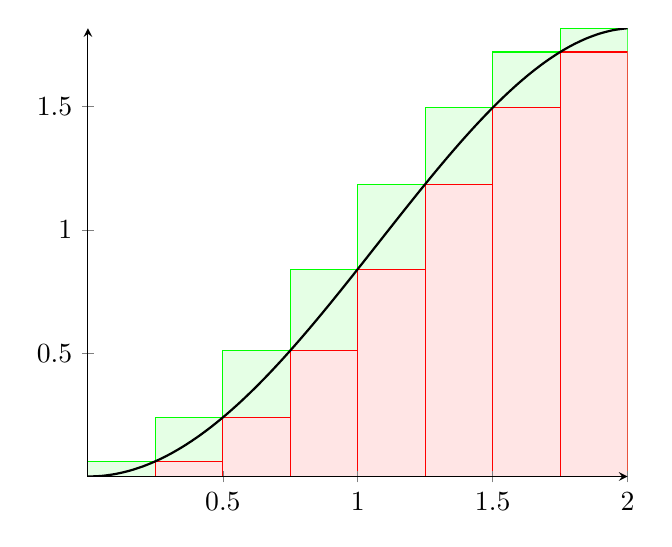
\begin{tikzpicture}[scale=1.0]
\begin{axis}[
    % xtick={0,...,1.5},ytick={0,...,1.5},
    % xmax=2,ymax=1.2,ymin=0,xmin=0,
    % enlargelimits=true,
    axis lines=middle,
    % clip=false,
    domain=0:2,
    axis on top
    ]

\addplot [draw=green, fill=green!10, const plot mark right, samples=9, domain=0:2]
    {x * sin(deg(x))}\closedcycle;
\addplot [draw=red, fill=red!10, ybar interval, samples=9, domain=0:2]
    {x * sin(deg(x))}\closedcycle;

\addplot[smooth, thick,domain=0:2,samples=40]{x * sin(deg(x))};
\end{axis}
\end{tikzpicture}
\caption{Somme di Riemann inferiori e superiori}
\end{figure}

Suddividiamo in un certo numero di rettangoli il sottografico della funzione. Disegnamo $n$ rettangoli, ciascuno con un area (data dalla base per l'altezza), e la somma delle aree \`e minore dell'area che vogliamo calcolare.

I punti scelti costituiscono una partizione dell'intervallo $[a,b]$. Se prendiamo una partizione pi\`u fitta, ottenendo quindi pi\`u rettangoli, la somma delle aree dei rettangoli \`e maggiore a quella precedente, ed \`e pi\`u vicina all'area che vogliamo calcolare.

Questa \`e l'idea di tal Cavalieri, il ``principio di esaustione''. Infittendo la partizione si approssima sempre meglio l'area sotto la curva.

Si pu\`o calcolare la somma delle aree dei rettangoli costruibili \emph{sopra} al grafico. L'area della somma di questi rettangoli \emph{contiene} l'area della funzione. In questo caso, infittendo la partizione, l'area diminuisce.

Vogliamo che queste due aree, quella sopra e quella sotto al grafico, siano, al limite, uguali. Se esiste un punto a cui queste due somme tendono, quel punto sar\`a proprio l'integrale.

\subsection{Somme di Riemann}

Consideriamo ora una funzione $f(x)$, e una partizione $P = \{ x_1, x_2, \ldots, x_n \}$ con $a = x_1 < x_2 < \ldots < x_{n-1} < x_n = b$.

Ora, per ogni coppia $[x_{i-1}, x_{i}]$ prendiamo due punti $l_i, u_i \in [x_{i-1}, x_{i}]$, tali che $f(l_i) \le f(x) \le f(u_i) \forall x \in [x_{i-1},x_{i}]$. I due punti $l_i$ e $u_i$ sono i punti di massimo e minimo della funzione nell'$i$-esimo intervallo.

Stiamo facendo l'ipotesi che in ciascuno di questi intervalli la funzione sia dotata di massimo e di minimo. Il teorema di Weierstrass ce lo garantisce, se la funzione \`e continua nell'intervallo.

Tenendo conto di queste notazioni, chiamiamo $L(P,f)$ la somma delle aree ``sotto'' la funzione, ossia:
\[
L(P,f) = \sum_{i = 1}^{n} f(l_i) \cdot (x_{i} - x_{i-1})
\]
Allo stesso modo, definiamo la somma $U(P,f)$ delle aree sopra la funzione:
\[
U(P,f) = \sum_{i = 1}^{n} f(u_i) \cdot (x_{i} - x_{i-1})
\]
\`E evidente che $L(P,f) \le U(P,f)$. Queste due quantit\`a si chiamano somme di Riemann, somma inferiore la prima e somma superiore la seconda.

Consideriamo due partizioni differenti, $P'$ e $P''$, vale sempre che $L(P',f) \le U(P'',f)$, anche se gli intervalli su cui ciascuna somma \`e basata sono differenti. Una somma fatta dal basso \`e sempre minore o uguale di una somma fatta dall'altro anche con una partizione differente.

Ora possiamo definire l'integrale definito, o integrale di Riemann.

\begin{defn}[Integrale di Riemann]
Se esiste un unico numero $I$ tale che $L(P',f) \le I \le U(P'',f) \forall P', P''$, allora $I$ sar\`a l'integrale di Riemann da $a$ a $b$:
\[
I = \int_{a}^{b} f(x) \dx
\]
\end{defn}
Questo \`e anche l'integrale definito, ma guai (per ora!) pensare di aver gi\`a visto il simbolo di integrale. \`E un simbolo con significato \emph{diverso} dal simbolo di integrale indefinito.

Come pu\`o succedere che non esista un unico numero $I$ che rispetta queste condizioni?

Consideriamo la funzione di Dirichlet, definita come segue:
\[
f(x) = 
\begin{cases}
1 \text{ se } x \in [0,1] \cap \rationals \\
0 \text{ se } x \notin [0,1] \setminus \rationals
\end{cases}
\]
Questa funzione non si pu\`o disegnare. Facciamo le somme di Riemann superiori e inferiori. In ogni intervallo abbiamo sia numeri razionali che numeri irrazionali. Il valore minimo della funzione \`e sempre 0, e il valore massimo \`e sempre 1, qualunque intervallo si scelga. Fra la somma inferiore e la somma superiore ci sono infiniti numeri, e non si pu\`o attribuire un'area al sottografico di questa funzione.

Se la funzione $f$ di cui vogliamo trovare l'area non \`e una funzione positiva nell'intervallo $[a,b]$ in cui cerchiamo l'area, che senso ha quello che stiamo facendo? Dobbiamo iniziare a parlare di \emph{area con segno}: consideriamo negativa un'area sotto l'asse delle $x$. I rettangoli che compongono la somma inferiore saranno pi\`u grandi dei rettangoli della somma superiore, ma attribuendogli un valore negativo la loro area resta minore dell'area dei rettangoli della somma superiore.

\begin{theorem}
\label{integrale_funzione_continua}
Se $f \in C^{0}([a,b])$ ($f$ \`e continua in $[a,b]$), allora esiste l'integrale definito $\int_{a}^{b} f(x) \dx$.
\end{theorem}

\begin{theorem}
Se $f \in C^{1}([a,b])$, ossia se $f$ \`e derivabile e $f'$ \`e continua in $[a,b]$, allora esiste l'integrale definito $\int_{a}^{b} f(x) \dx$.
\end{theorem}
Dimostrarlo per esercizio.

La scrittura $f \in C^{n} ([a,b])$ indica che la funzione $f$ \`e continua, \`e derivabile $n$ volte nell'intervallo $[a,b]$, e ognuna delle $n$ derivate \`e continua in $[a,b]$.

\begin{theorem} \label{integrabilita_riemann}
Usando le somme di Riemann si pu\`o stabilire se esiste l'integrale di Riemann.
\[
\exists \int_{a}^{b} f(x) \dx \iff \forall \epsilon > 0 \exists P \text{ t.c. } U(P,f) - L(P,f) < \epsilon
\]
Ossia, una funzione ha integrale di Riemann se e solo se la differenza fra le due somme (superiore e inferiore) pu\`o essere resa arbitrariamente piccola (con un'opportuna partizione).
\end{theorem}

\begin{oss}
Data una partizione $P$ di $[a,b]$, sia $c_i \in [x_{i-1},x_i]$ un punto qualunque nell'$i$-esimo intervallo determinato dalla partizione. Osserviamo che $f(l_i) \le f(c_i) \le f(l_i)$. Possiamo quindi scrivere che:
\[
L(P,f) = \sum_{i = 1}^{n} f(l_i) \cdot (x_{i} - x_{i - 1}) \le \sum_{i = 1}^{n} f(c_i) \cdot (x_{i} - x_{i - 1}) \le \sum_{i = 1}^{n} f(u_i) \cdot (x_{i} - x_{i - 1}) = U(P,f)
\]
\`E chiaro che se la funzione \`e integrabile, la somma di mezzo viene \emph{schiacciata} dalle altre due.
\end{oss}

Con questa osservazione possiamo tirare fuori una versione diversa del teorema \ref{integrabilita_riemann}.
\[
\int_{a}^{b} f(x) \dx = \lim_{\norm{P} \to 0} \sum_{i = 1}^{n} f(c_i) \cdot (x_i - x_{i - 1})
\]
La norma di $P$ ($\norm{P}$) \`e la massima lunghezza di un intervallo, ossia $\norm{P} = \max(x_i - x_{i-1})$.

% L'area del sottografico \`e l'area compresa fra il grafico e l'asse delle $x$. Se l'asse $x$ \`e sopra il grafico, l'area per convenzione ha segno negativo.

% L'integrale di una funzione dispari su un intervallo simmetrico rispetto all'asse $y$ \`e sempre nullo.

\subsection{Considerazioni sugli integrali definiti}

Per definizione, con gli integrali definiti vale:
\[
\int_{b}^{a} f(x) \dx = - \int_{a}^{b} f(x) \dx
\]
Facciamo qualche considerazione pi\`u o meno banale.
\begin{enumerate}
    \item Se $f(x) \le g(x)$ in $[a,b]$, allora:
    \[
    \int_{a}^{b} f(x) \dx \le \int_{a}^{b} g(x) \dx
    \]
    \item L'integrale definito \`e lineare:
    \[
    \int_{a}^{b} \left[ A \, f(x) + B \, g(x) \right] \dx =
    A \int_{a}^{b} f(x) \dx + B \int_{a}^{b} g(x) \dx
    \]
    Vederlo in maniera geometrica non \`e immediato. Ma abbiamo visto che le derivate sono lineari, visto che le derivate sono limiti e i limiti a loro volta sono lineari. Scriviamo questo integrale come limite, considerando una partizione $P = \{ x_1, x_2, \ldots, x_n \}$ e i punti $c_i \in [x_{i-1}, x_{i}]$:
    \[
    \lim_{\norm{P} \to 0} \sum_{i = 1}^{n} \left[ A \, f(c_i) + B \, g(c_i) \right] \cdot (x_{i} - x_{i-1})
    \]
    Ma il limite della combinazione lineare, abbiamo detto, \`e la combinazione lineare dei limiti:
    \[
    A \, \lim_{\norm{P} \to 0} \sum_{i = 1}^{n} f(c_i) \cdot (x_{i} - x_{i - 1}) +
    B \, \lim_{\norm{P} \to 0} \sum_{i = 1}^{n} g(c_i) \cdot (x_{i} - x_{i - 1})
    \]
    Questa quantit\`a \`e esattamente $A$ volte l'integrale definito di $f(x)$ pi\`u $B$ volte l'integrale definito di $g(x)$.
    \item Se $a < c < b$ ed esiste l'integrale definito $\int_{a}^{b} f(x) \dx$, allora:
    \[
    \int_{a}^{b} f(x) \dx = \int_{a}^{c} f(x) \dx + \int_{c}^{b} f(x) \dx
    \]
    \item Vale questa propriet\`a:
    \[
    \abs{\int_{a}^{b} f(x) \dx} \le \int_{a}^{b} \abs{f(x) \dx}
    \]
    \`E simile alla tipica disuguaglianza triangolare: $\abs{a + b} \le \abs{a} + \abs{b}$.
    \item Considerando integrali definiti su intervalli simmetrici rispetto all'asse $y$, se $f$ \`e pari vale che:
    \[
    \int_{-b}^{b} f(x) \dx = 2 \, \int_{0}^{b} f(x) \dx
    \]
    Se \`e dispari, vale invece che:
    \[
    \int_{-b}^{b} f(x) \dx = 0
    \]
\end{enumerate}

\subsubsection{Teorema del valor medio applicato agli integrali definiti}

Consideriamo un integrale definito di una funzione continua:
\[
\int_{a}^{b} f(x) \dx
\]
Siano, per il teorema di Weierstrass, $m = \min_{[a,b]} f(x)$ e $M = \max_{[a,b]} f(x)$. Possiamo minorare e maggiorare l'integrale definito come segue:
\[
\int_{a}^{b} m \dx \le \int_{a}^{b} f(x) \dx \le \int_{a}^{b} M \dx
\]
Si vede facilmente che $\int_{a}^{b} M \dx = M \cdot (b - a)$, e quindi che:
\[
m \cdot (b - a) \le \int_{a}^{b} f(x) \dx \le M \cdot (b - a) \implies
m \le \frac{1}{b - a} \int _{a}^{b} f(x) \dx \le M
\]
La funzione \`e continua per ipotesi, quindi assume tutti i valori fra minimo e massimo. Questo vuol dire che $\exists c \in (a,b)$ tale per cui:
\[
\frac{1}{b - a} \int_{a}^{b} f(x) \dx = f(c)
\]
Geometricamente, vuol dire che l'area sotto la funzione \`e uguale all'area del rettangolo alto $f(c)$ e largo quanto l'intervallo preso in esame, anche se non conosciamo dove sia il punto $c$.

\begin{exmp}
Consideriamo l'integrale definito $\int_{0}^{2} x \dx$, e la partizione $P_n$ dell'intervallo $[0,2]$ in sottointervalli ciascuno di lunghezza $\frac{2}{n}$. La differenza fra le somme inferiori e superiori di Riemann \`e:
\[
U(P_n, f) - L(P_n, f) = \sum_{i = 1}^{n} \left[ f(u_i) - f(l_i) \right] \cdot \frac{2}{n} = n \cdot \frac{4}{n^2}
\]
L'integrale definito di questa funzione, in questo intervallo, esiste: $\forall \epsilon > 0, \exists N_{\epsilon}$ tale per cui la differenza sopra \`e minore di $\epsilon$, per ogni $n \ge N_{\epsilon}$. Infatti basta che valga:
\[
n > \frac{4}{\epsilon}
\]
Si pu\`o poi far vedere quanto vale questo integrale definito, trovando i limiti delle somme inferiori o delle somme superiori.
\[
\int_{0}^{2} x \dx = 2 = \lim_{n \to \infty} U(P_n, f) = \lim_{n \to \infty} L(P_n, f)
\]
Infatti:
\[
\lim_{n \to \infty} U(P_n,f) = 
\lim_{n \to \infty} \sum_{i = 1}^{n} \frac{i \, 2}{n} \cdot \frac{2}{n} = \lim_{n \to \infty} \frac{4}{n^2} \cdot \sum_{i = 1}^{n} i =
\lim_{n \to \infty} \frac{\cancelto{2}{4}}{\cancel{n^2}} \cdot \frac{\cancel{n^2} + \cancelto{0}{n}}{\cancel{2}} = 2
\]
\end{exmp}

Salvo in casi particolari, l'unico modo per calcolare integrali definiti \`e attraverso l'approssimazione.

\section{Teorema fondamentale del calcolo}

Il teorema fondamentale del calcolo vale per ogni $f \in C^{0} ([a,b])$ (ossia per ogni funzione continua nell'intervallo chiuso e limitato $[a,b]$).

\begin{theorem}[Teorema fondamentale del Calcolo]
Sia $F(x) = \int_{a}^{x} f(t) \dx[t]$, per $a \le x \le b$, ossia la funzione che calcola l'area sotto il grafico della funzione $f$ dal punto $a$ al punto (variabile) $x$, allora:
\begin{enumerate}
    \item $\exists F'(x) = f(x)$
    \item $\forall G$ primitiva di $f$ in $[a,b]$, risulta che:
    \[
    \int_{a}^{b} f(x) \dx = G(b) - G(a) = \increment{\int f(x) \dx}_{a}^{b}
    \]
    L'ultima parte si legge ``incremento dell'integrale indefinito da $a$ a $b$''.
\end{enumerate}
\end{theorem}
Nella premessa, $x$ indica l'estremo superiore di integrazione, mentre la $t$ \`e una variabile muta di integrazione (e quindi non \`e minimamente rilevante la lettera che gli si associa).

La nozione di primitiva di una funzione e quella di area individuata dal grafo della funzione sono legate a doppio filo dal teorema fondamentale del Calcolo.

\begin{proof}
Calcoliamo la derivata della funzione $F(x)$.
\begin{align*}
\lim_{h \to 0} \frac{F(x + h) - F(x)}{h} = 
\lim_{h \to 0} \frac{1}{h} \, \left[ \int_{a}^{x+h} f(t) \dx[t] - \int_{a}^{x} f(t) \dx[t] \right] = \tag{per additivit\`a degli integrali} \\
= \lim_{h \to 0} \frac{1}{h} \, \left[ \cancel{\int_{a}^{x} f(t) \dx[t]} + \int_{x}^{x+h} f(t) \dx[t] - \cancel{\int_{a}^{x} f(t) \dx[t]} \right]
= \lim_{h \to 0} \frac{1}{h} \, \int_{x}^{x+h} f(t) \dx[t] = \tag{per il valor medio} \\
= \lim_{h \to 0} \frac{1}{h} \cdot f(c) \cdot (\cancel{x} + h - \cancel{x}) = \lim_{h \to 0} f(c) \cdot \frac{\cancel{h}}{\cancel{h}} = \lim_{h \to 0} f(c)
\end{align*}
Con $c \in [x, x+h]$, ma per $h \to 0$, si ha che $c \to x$, e quindi la derivata di $F(x)$ (che \`e la funzione che calcola l'area sotto $f(x)$) \`e proprio $f(x)$. 

Vediamo poi che se $G'(x) = f(x)$, allora $G(x) + c = \int_{a}^{x} f(t) \dx[t]$. Cosa segue da questo?

Prima di tutto, prendendo $x = a$, si ha che $G(a) + c = 0$, e quindi $c = - G(a)$.

Poi, prendendo $x = b$, abbiamo che $\int_{a}^{b} f(t) \dx[t] = G(b) + c = G(b) - G(a)$. E quindi una qualsiasi primitiva di $f(x)$ \`e la funzione che calcola l'area sotto il grafico di $f(x)$!
\end{proof}

\subsection{Integrali definiti e derivate}
\label{derivate_di_integrali}

Abbiamo detto che se $f \in C^0 ([a,b])$, ossia se \`e continua in $[a,b]$, allora $f$ \`e integrabile in $[a,b]$, e in particolare per ogni punto $x \in [a,b]$:
\[
F(x) = \int_{a}^{x} f(x) \dx
\]
Facendo variare il punto $x$ si ottiene una funzione che dipende da $x$. Il teorema fondamentale del calcolo integrale ci dice che questa funzione $F(x)$ \`e derivabile, e la derivata \`e la funzione integranda $f(x)$.

Cosa vuol dire questo?
\[
G(x) = \int_{a}^{x^2} f(t) \dx[t]
\]
Vuol dire che $G(x) = F(x^2)$. Infatti, se sostituiamo nell'equazione che segue $y$ con $x^2$, otteniamo la stessa cosa.
\[
F(y) = \int_{a}^{y} f(t) \dx[t]
\]
Se deriviamo $G(x)$ cosa succede?
\[
\deriv{x} G(x) = \deriv{x} F(x^2) = 2 \, x \, f(x^2)
\]
Basta applicare la regola di derivazione delle funzioni composte.

Una nota pedante sulla derivata delle funzioni composte. La derivata di una funzione, come $F(x^2)$, si scrive come la derivata della funzione ``esterna'' $F$ \emph{calcolata} in $x^2$ per la derivata della funzione ``interna'', $x^2$. Si scrive cos\`i:
\[
\deriv{x} F(x^2) = \left( \deriv{y} F \right) \left( x^2 \right) \cdot \deriv{x} \left( x^2 \right)
\]

\begin{exmp}
Guardiamo questa funzione:
\[
G(x) = \int_{0}^{\sin(x)} \frac{1}{1 + t^2} \dx[t]
\]
La sua derivata $G'(x)$ \`e:
\[
G'(x) = \frac{\cos(x)}{1 + \sin^2(x)} = \frac{\cancel{\cos(x)}}{\cos^{\cancel{2}}(x)} = \frac{1}{\cos(x)}
\]

Guardiamo questa:
\[
G(x) = \int_{a}^{\tan \left[ \log(1 + x^2) \right]} \arctan \left[ e^{t^2 + \cos(t)} \right] \dx[t]
\]
Non possiamo neanche lontanamente pensare di trovare l'integrale di questo mostro. Noi vogliamo solo calcolare $G'(x)$. Si prende la funzione integranda e la si calcola nell'estremo superiore, e la si moltiplica per la derivata dell'estremo superiore.
\begin{align*}
G'(x) &= \arctan \left[ e^{{\tan \left[ \log(1 + x^2) \right]}^2 + \cos \left( \tan \left[ \log(1 + x^2) \right] \right)} \right] \cdot \left[ \tan \left[ \log(1 + x^2) \right] \right]' = \\
&= \arctan \left[ e^{{\tan \left[ \log(1 + x^2) \right]}^2 + \cos \left( \tan \left[ \log(1 + x^2) \right] \right)} \right] \cdot \frac{1}{\cos^2 \left[ \log(1 + x^2) \right]} \cdot \frac{1}{1 + x^2} \cdot 2 \, x
\end{align*}

Questi esempi infami servono a capire cosa significa il teorema fondamentale del calcolo, ossia che l'integrale $\int_{a}^{x} f(t) \dx[t] = F(x)$ \`e tale che $F'(x) = f(x)$. Quindi la derivata di questo integrale \`e immediata:
\[
\deriv{x} \int_{a}^{x} \cos (\tan(1 + t^2)) \cdot e^{\arctan(\log(1+t^{2 \, \cos^2(t)}))} \dx[t] = 
\cos (\tan(1 + x^2)) \cdot e^{\arctan(\log(1+x^{2 \, \cos^2(x)}))}
\]
Per calcolare la derivata della funzione $F(x)$ non dobbiamo conosccere la funzione $F(x)$, perch\'e conosciamo la funzione $f(x)$.

E se volessimo derivare un integrale che ha delle funzioni in entrambi gli estremi di integrazione?
\[
G(x) = \int_{\tan(x^2)}^{e^{2x + \cos^2(x)}} \left[ t^a + \log(1 + t^2) \right] \dx[t]
\]
A esser precisi bisognerebbe dire che la $x$ \`e compresa fra $- \frac{\pi}{2}$ e $\frac{\pi}{2}$. Comunque, sappiamo come spezzare questo integrale:
\[
G(x) = \int_{0}^{e^{2x + \cos^2(x)}} \left[ t^a + \log(1 + t^2) \right] \dx[t] - \int_{0}^{\tan(x^2)} \left[ t^a + \log(1 + t^2) \right] \dx[t]
\]
Si possono scambiare gli estremi di integrazione invertendo il segno dell'integrale. Adesso sapppiamo come calcolare la derivata di $G(x)$.
\begin{align*}
G'(x) =& e^{2a \, x + a \, \cos^2(x)} + \log(1 + e^{4 \, x + 2 \, \cos^2(x)}) \cdot e^{2 \, x + \cos^2 (x)} \cdot \left( 2 - 2 \, \sin(x) \cos(x) \right) + \\
&-  {\tan(x^2)}^a + \log(1 + {\tan(x^2)}^2) \cdot \frac{1}{\cos^2(x)} \cdot 2 \, x
\end{align*}

In questo caso non abbiamo assolutamente modo di trovare la primitiva di $f(x)$:
\[
G(x) = \int_{\sin(x)}^{\cos^2(x)} e^{-t^2} \dx[t]
\]
Ma sappiamo sempre trovare la derivata di $G(x)$.
\[
G'(x) = e^{-{\left[ \cos^2(x) \right]}^2} \cdot (- 2 \sin(x) \cos(x)) - 
e^{-\sin^2(x)} \cdot \cos(x)
\]
\end{exmp}

Se adesso vogliamo tirare fuori un caso generale, possiamo scrivere che, dato questo integrale:
\[
G(x) = \int_{\alpha (x)}^{\beta (x)} f(t) \dx[t]
\]
la sua derivata \`e:
\[
G'(x) = f(\beta(x)) \cdot \beta'(x) - f(\alpha(x)) \cdot \alpha'(x)
\]
per il teorema fondamentale del calcolo.

\subsection{Funzioni continue a tratti}

Un esempio di funzione continua a tratti \`e la funzione parte intera.
\[
f(x) = \left[ x \right]
\]
Supponiamo ora di voler calcolare l'integrale:
\[
\int_{\frac{3}{2}}^{4} \left[ x \right] \dx
\]
\begin{figure}[h]
\centering
\begin{tikzpicture}
    \begin{axis}[
            xmin=0,xmax=5,
            ymin=0,ymax=5,
            axis x line=middle,
            axis y line=left,
            axis line style={->},
            % xlabel={$\reals$},
        ]
        \addplot[line width=2pt,-,domain=0:1]{0};
        \addplot[line width=2pt,-,domain=1:2]{1};
        \addplot[line width=2pt,-,domain=2:3]{2};
        \addplot[line width=2pt,-,domain=3:4]{3};
        \addplot[line width=2pt,-,domain=4:5]{4};
        \addplot[fill=black,only marks,mark=*]coordinates{(0,0)(1,1)(2,2)(3,3)(4,4)};
    \end{axis}
\end{tikzpicture}
\caption{La funzione ``parte intera''}
\end{figure}

La funzione non \`e continua, e non \`e continua neanche nell'intervallo [1,2]. \`E continua solo nell'intervallo [1,2) che ha un estremo non chiuso! Ma l'area sotto il rettangolo [1,2] \`e identica all'area sotto il rettangolo [1,2), poich\'e differiscono di un solo segmento.

Quindi l'integrale che abbiamo visto vale:
\[
\int_{\frac{3}{2}}^{4} \left[ x \right] \dx =
\int_{\frac{3}{2}}^{2} \left[ x \right] \dx +
\int_{2}^{3} \left[ x \right] \dx +
\int_{3}^{4} \left[ x \right] \dx
\]

\section{Integrali impropri}

Sappiamo calcolare l'integrale indefinito di:
\[
\int \log (x) \dx = x \, \log (x) - x + c
\]
Poi, $\forall a \ge 0$, sappiamo calcolare questo integrale definito:
\[
\int_{a}^{1} \log (x) \dx = - 1 - a \, \log (a) + a
\]
Facendo il limite per a che tende a $0^+$, vediamo che quest'area vale:
\[
\lim_{a \to 0^+} \int_{a}^{1} \log (x) \dx = -1
\]
Sappiamo calcolare qualunque area di questo tipo, $\forall a, b \ge 0$:
\[
\int_{a}^{b} \log (x) \dx
\]
Abbiamo parlato solo di intervalli $[a,b]$ chiusi e limitati. La cosa pi\`u estrema che abbiamo fatto \`e stato togliere un punto dall'estremo dell'intervallo. Ma in questo caso, se studiamo $\log (x)$ nell'intervallo $(0,1]$, la funzione \`e continua \emph{ma non} limitata.

Prendendo per\`o un qualunque $a \in (0,1]$, la funzione nel punto $a$ \`e sia continua che limitata. Facendo tendere $a$ a $0^+$ vediamo che l'area sotto la funzione \`e limitata, e tende a $-1$. La cosa rilevante \`e che abbiamo attribuito un'area limitata al grafico di una funzione su un insieme illimitato. Adesso possiamo ammettere questo:
\[
\int_{0}^{1} \log (x) \dx = -1
\]
Questo \`e un integrale improprio. Un integrale improprio \`e il limite di un integrale proprio.

\begin{exmp}
Quello che segue \`e un normale integrale definito, per $b \in \reals$.
\[
\int_{1}^{b} \frac{\diff x}{1 + x^2} = \arctan (b) - \frac{\pi}{4}
\]
Ma se facciamo il limite per $b \to \infty$, l'integrale diventa un integrale improprio.
\[
\lim_{b \to \infty} \int_{1}^{b} \frac{\diff x}{1 + x^2} = \frac{\pi}{2} - \frac{\pi}{4} = \frac{\pi}{4}
\]
\end{exmp}

\begin{exmp}
Questo \`e immediatamente riconoscibile come un integrale improprio:
\[
\int_{0}^{1} \frac{\diff x}{x}
\]
La funzione integranda, infatti, non \`e definita in uno degli estremi di integrazione (nello specifico, in 0). Quindi trovare un integrale simile vuol dire trovare questo integrale:
\[
\lim_{a \to 0^+} \int_{a}^{1} \frac{\diff x}{x} =
\lim_{a \to 0^+} \log(1) - \log(a) = 
- \lim_{a \to 0^+} \log(a) = \infty
\]
Qui abbiamo quindi una funzione illimitata su un intervallo limitato, e il suo integrale non esiste.
\end{exmp}

\begin{exmp}
Variazioni sullo stesso integrale improprio.
\[
\int_{1}^{\infty} \frac{\diff x}{x}
\]
Anche questo \`e improprio. Abbiamo una funzione integranda che (in $[1, \infty)$) \`e limitata, nonostante l'intervallo preso non lo sia.
\[
\lim_{b \to \infty} \int_{1}^{b} \frac{\diff x}{x} = \lim_{b \to \infty} \log(b) = \infty
\]
\end{exmp}

Quindi l'integrale definito di $\frac{1}{x}$ non esiste n\'e fra 0 e 1, n\'e fra 1 e $\infty$. $\frac{1}{x}$ \`e una funzione illimitata in 0 e all'infinito. Sar\`a sempre cos\`i, con tutte le funzioni non limitate?

\begin{exmp}
L'integrale che segue sembra simile ai casi precedenti, ma... 
\[
\int \frac{\diff x}{x^2} = - \frac{1}{x} + c
\]
Rifacciamo entrambi i ``test'' fatti prima.
\begin{align*}
\int_{0}^{1} \frac{\diff x}{x^2} \\
\int_{1}^{\infty} \frac{\diff x}{x^2}
\end{align*}
Sempre due integrali impropri. Ma vogliamo capire quale integrale converge e quale diverge.
\[
\lim_{a \to 0^+} \int_{a}^{1} \frac{\diff x}{x^2} =
\lim_{a \to 0^+} - 1 + \frac{1}{a} = \infty
\]
Diverge fra 0 e 1...
\[
\lim_{b \to \infty} \int_{1}^{b} \frac{\diff x}{x^2} =
\lim_{b \to 0^+} - \frac{1}{b} + 1 = 1
\]
E converge a 1 fra 1 e $\infty$.
\end{exmp}

\begin{exmp}
Vediamo un altro caso apparentemente simile ai precedenti. 
\[
\int \frac{\diff x}{\sqrt{x}} = 2 \, \sqrt{x} + c
\]
Quale integrale improprio converge, e quale diverge?
\[
\lim_{a \to 0^+} \int_{a}^{1} \frac{\diff x}{\sqrt{x}} =
\lim_{a \to 0^+} 2 - 2 \, \sqrt{a} = 2
\]
Converge (a 2) fra 0 e 1...
\[
\lim_{b \to \infty} \int_{1}^{b} \frac{\diff x}{\sqrt{x}} =
\lim_{b \to 0^+} 2 \, \sqrt{b} - 2 = \infty
\]
E diverge fra 1 e $\infty$.
\end{exmp}

\subsection{Funzioni razionali e integrali impropri}
\label{integrali_impropri_razionali}

Conosciamo l'integrale di questa funzione generica:
\[
\int \frac{\diff x}{x^p} = 
\begin{cases}
\dfrac{x^{-p + 1}}{- p + 1} + c & \text{ se } p \neq 1 \\
\abslog{x} + c & \text{ se } p = 1
\end{cases}
\]
Vogliamo studiare due integrali impropri a partire da questa funzione generica.
\begin{align*}
\int_{0}^{1} \frac{\diff x}{x^p} \qquad
\int_{1}^{\infty} \frac{\diff x}{x^p}
\end{align*}
\`E chiaro che, per $p$ negativo o nullo ($p \le 0$), il primo \`e un integrale proprio (la funzione, infatti, \`e continua e limitata anche in 0). I casi interessanti sono quelli per $p > 0$. Vogliamo capire per quali valori di $p$ questo integrale converge e per quali diverge.

Abbiamo visto che se $p = \frac{1}{2}$ il primo converge, il secondo diverge, mentre se $p = 2$ il primo diverge e il secondo converge.

Vediamo il primo integrale improprio nel caso generico, per $p \neq 1$:
\[
\int_{0}^{1} \frac{\diff x}{x^p} = 
\lim_{a \to 0^+} \int_{a}^{1} \frac{\diff x}{x^p} =
\lim_{a \to 0^+} \frac{1}{- p + 1} - \frac{a^{-p + 1}}{-p + 1}
\]
Ora, tutto dipende da $-p + 1$. Per a che tende a $0^+$, $a^n$ tende a $0$ se l'esponente \`e positivo, o a $\infty$ se l'esponente \`e negativo. Quindi:
\[
\lim_{a \to 0^+} \frac{1}{- p + 1} - \frac{a^{-p + 1}}{-p + 1} =
\begin{cases}
\dfrac{1}{- p + 1} & \text{ se } p < 1 \\
\infty & \text{ se } p > 1
\end{cases}
\]
Se $p < 1$, abbiamo che $-p > - 1 \implies - p + 1 > 0$.

Vediamo l'altro integrale.
\[
\int_{1}^{\infty} \frac{\diff x}{x^p} =
\lim_{b \to \infty} \int_{1}^{b} \frac{\diff x}{x^p} = 
\begin{cases}
\text{qualcosa} \in \reals & \text{ se } p > 1 \\
\infty & \text{ se } p \le 1
\end{cases}
\]

\subsubsection{Recap}

Nell'intervallo $\ocint{0}{1}$ vale questo:
\[
\int_{0}^{1} \frac{\diff x}{x^p} = 
\begin{cases}
\dfrac{1}{- p + 1} & \text{ se } p < 1 \\
\infty & \text{ se } p \ge 1
\end{cases}
\]
Nell'intervallo $\coint{1}{\infty}$ vale questo:
\[
\int_{1}^{\infty} \frac{\diff x}{x^p} =
\begin{cases}
\text{qualcosa} \in \reals & \text{ se } p > 1 \\
\infty & \text{ se } p \le 1
\end{cases}
\]
E basta.

\begin{exmp}
Basta integrali impropri di funzioni razionali.
\[
\int_{0}^{\infty} x \, e^{-x} \dx =
\lim_{b \to \infty} \int_{0}^{b} x \, e^{-x} \dx = 
\increment{\lim_{b \to \infty} -x \, e^{-x} - e^{-x}}_{0}^{b} =
\lim_{b \to \infty} -b \, e^{-b} - e^{-b} + 1 = + 1
\]
\end{exmp}

\begin{exmp}
Studiamo questo integrale improprio:
\[
\int_{- \infty}^{\infty} e^{-\abs{x}} \dx
\]
La funzione \`e pari, ed \`e limitata. La scriviamo come somma di due integrali impropri:
\begin{align*}
\int_{0}^{\infty} e^{-x} \dx + \int_{-\infty}^{0} e^{x} \dx =
2 \, \int_{0}^{\infty} e^{-x} \dx &= \\
2 \, \lim_{b \to \infty} \int_{0}^{b} e^{-x} \dx = 
\increment{2 \, \lim_{b \to \infty} - e^{-x}}_{0}^{b} = 
2 \, \lim_{b \to \infty} - e^{-b} + e^{0} &= 2
\end{align*}
\end{exmp}

\subsection{Criterio del confronto per determinare la convergenza}

Non tutti gli integrali sono simpatici, non di tutti gli integrali sappiamo trovare l'integrale indefinito.
\[
\int_{0}^{\infty} e^{-x^2} \dx
\]
Non serve a molto riscriverlo cos\`i:
\[
\lim_{b \to \infty} \int_{0}^{b} e^{-x^2} \dx
\]
perch\'e non sappiamo trovare l'integrale indefinito! Ma possiamo usare un criterio del confronto, dicendo prima questo:
\[
e^{-x^2} \le e^{-x}
\]
e quindi:
\[
\lim_{b \to \infty} \int_{0}^{b} e^{-x^2} \dx \le
\lim_{b \to \infty} \int_{0}^{b} e^{-x} \dx = 1
\]

Sono sempre e solo due le cose che si possono fare, per vedere se un integrale improprio converge o diverge:
\begin{enumerate}
    \item maggiorare l'integrale dato con un integrale che converge, e scoprire quindi che l'integrale dato converge, oppure
    \item minorare l'integrale dato con un integrale che diverge, e scoprire quindi che l'integrale dato diverge.
\end{enumerate}

\begin{exmp}
Scopriamo se questo integrale (improprio) converge o diverge.
\[
\int_{-1}^{0} \frac{e^x}{x+1} \dx
\]
\`E improprio, perch\'e per $x$ che tende a $-1$ la funzione integranda tende all'infinito. In 0 la funzione \`e definita (e vale 1).

Si pu\`o vedere che vale questa disuguaglianza, sapendo che $e^0$ vale 1:
\[
\frac{e^x}{x+1} \le \frac{1}{x+1} \text{ per } x \in \ocint{-1}{0}
\]
Infatti sappiamo che $e^x$ in $\ocint{-\infty}{0}$ \`e crescente, con massimo in $0$, e il massimo vale 1. Quindi $e^x$ in $\ocint{-\infty}{0}$ si maggiora con 1!

Per\`o \`e una maggiorazione inutile, visto che la funzione con cui abbiamo maggiorato la funzione integranda \emph{non ha} un integrale convergente.

Ma in $\ccint{-1}{0}$ la funzione $e^x$ ha il minimo in $-1$, e quel minimo \`e $e^{-1}$. Quindi la funzione integranda possiamo minorarla cos\`i:
\[
\frac{e^{-1}}{x+1} \le \frac{e^x}{x+1} \text{ per } x \in \ocint{-1}{0}
\]
La funzione con cui abbiamo minorato \`e simile alla funzione con cui abbiamo maggiorato prima (\`e la funzione di prima moltiplicata per la costante $e^{-1}$), quindi anche l'integrale di questa funzione diverge. Avendo minorato, in questo caso, abbiamo capito che l'integrale improprio iniziale \emph{diverge}.
\end{exmp}

C'\`e una certa disuguaglianza molto importante:
\[
0 \le \frac{\sin(x)}{x} \le 1
\]

\begin{exmp}
La disuguaglianza serve per determinare la convergenza di questo integrale:
\[
\int_{0}^{\frac{\pi}{2}} \frac{\sin(x)}{x^{\frac{7}{4}}} \dx
\]
Prima vediamo qualcosa di sbagliato, sapendo che vale sempre $\sin(x) \le 1$:
\[
\int_{0}^{\frac{\pi}{2}} \frac{\sin(x)}{x^{\frac{7}{4}}} \dx \le
\int_{0}^{\frac{\pi}{2}} \frac{\diff x}{x^{\frac{7}{4}}}
\]
Ma questo diverge. Non serve a niente maggiorare con qualcosa che diverge.

Invece possiamo maggiorarlo con qualcosa che converge:
\[
\int_{0}^{\frac{\pi}{2}} \frac{\sin(x)}{x^{\frac{7}{4}}} \dx =
\int_{0}^{\frac{\pi}{2}} \frac{\sin(x)}{x} \, \frac{\diff x}{x^{\frac{3}{4}}} \le
\int_{0}^{\frac{\pi}{2}} \frac{\diff x}{x^{\frac{3}{4}}}
\]
E quest'ultimo, per le regole viste nella sezione \ref{integrali_impropri_razionali}, converge.
\end{exmp}

\begin{exmp}
Questo integrale:
\[
\int_{1}^{\infty} \frac{x \, \arctan(x)^2}{x^3 + \log(x)} \dx
\]
Maggioriamo il numeratore e minoriamo il denumeratore, per maggiorare tutto l'integrale:
\[
\frac{x \, \arctan(x)^2}{x^3 + \log(x)} \le \frac{x \cdot \left( \frac{\pi}{2} \right)^2}{x^3}
\]
Questo \`e simile a un integrale del tipo $\frac{1}{x^2}$, che sappiamo convergere in $\coint{1}{\infty}$. A posto.
\end{exmp}
















\clearpage

\chapter{Equazioni differenziali}

La forma generale delle equazioni differenziali \`e:
\[
y' = f(t,y)
\]
Le soluzioni saranno tutte le funzioni $y(t)$ tali che $y'(t) = f(t, y(t)) \forall t$.

Facciamo un esempio: l'accelerazione \`e la derivata seconda dello spostamento. Quindi il secondo principio della dinamica (forza = massa per accelerazione) si pu\`o scrivere come:
\[
f(t, y, y') = F = m \cdot a = m \cdot y''
\]
indicando con $y(t)$ lo spostamento al tempo $t$. La forza \`e una funzione dell'istante, dello spostamento e della velocit\`a.

Il caso pi\`u semplice che possiamo affrontare \`e:
\[
y' = a \cdot y
\]
\`E, ad esempio, l'equazione che governa il decadimento radioattivo. E si potrebbe usare per trovare l'equazione di crescita di una popolazione, indicando con $a$ il tasso di natalit\`a meno il tasso di mortalit\`a. O almeno, questa legge \emph{dovrebbe} governare il tasso di crescita (o decrescita) di una popolazione.

Una funzione che verifica $y' = a \cdot y$, per $a = 1$, \`e $e^x$. Generalizzando, ovviamente, la funzione \`e $e^{a \cdot x}$.

Quindi, $y = C \, e^{a \cdot t}$ rappresenta le infinite soluzioni di $y' = a \cdot y$. \`E facilmente verificabile. Ma noi vogliamo una soluzione unica. L'univocit\`a della risposta dipende dal \emph{dato iniziale}. Se stiamo considerando, ad esempio, una popolazione, il numero della popolazione in un certo istante $t'$ dipende dal numero della popolazione all'istante iniziale $t_0$.

Si vede subito che la funzione, all'istante iniziale, vale $y(0) = C$.

\section{Problemi di Cauchy}

Si chiama \emph{problema di Cauchy} la combo di equazione differenziale e valore iniziale:
\[
y' = a \cdot y , \, y(0) = C
\]
La soluzione (ossia la funzione $y$) \`e univoca.

Un'equazione del genere, usata per descrivere la crescita di una popolazione, \`e chiamato \emph{modello maltusiano}.

In realt\`a, l'andamento di una popolazione \`e descritta meglio da un'equazione differenziale del tipo:
\[
y' = a \, y - b \, y^2
\]
detta \emph{equazione logistica}.

Queste sono dette equazioni differenziali del primo ordine. Equazioni differenziali del secondo ordine sono equazioni differenziali contenenti una derivata seconda, come l'equazione differenziale vista all'inizio, per il secondo principio della dinamica, o l'equazione che descrive l'andamento di una molla.

%y'' = y + \omega^2
% CONTROLLARE

\subsubsection{Equazioni differenziali banali}

Un'equazione differenziale del primo ordine molto banale \`e:
\[
y' = f(t)
\]
Non merita neanche di essere chiamata un'equazione differenziale: il problema \`e soltanto trovare le primitive di $f(t)$. Le primitive sono infinite, e questo lo sappiamo. Le soluzioni sono del tipo:
\[
y(t) = \int f(t) \dx[t] = \int_{t_0}^{t} f(s) \dx[s] + C
\]
Per rendere una ricerca di primitive un problema di Cauchy, si deve imporre una condizione del tipo $y(t_0) = y_0$ (detta \emph{condizione di Cauchyt}). Ponendo $t = t_0$, l'integrale \`e 0, e quindi deve essere $C = y_0$. 

Quindi la soluzione generale di $y' = f(t)$ (con condizione di Cauchy $y(t_0) = y_0$) \`e:
\[
y(t) = \int_{t_0}^{t} f(s) \dx[s] + y_0
\]
Fine.

Le equazioni differenziali \emph{banali} sono quelle in cui il secondo membro non dipende dall'incognita, ossia quelle, come appena visto, nella forma:
\[
y' = f(t)
\]
Le equazioni differenziali (del primo ordine) interessanti sono tutte:
\[
y' = f(y)
\]
Torniamo al caso particolare in cui $f(y) = a \, y$. Una funzione che vale identicamente 0 \`e soluzione dell'equazione. Escludiamo questo caso, e scriviamo questo (nei punti in cui $y$ \`e diversa da 0):
\[
y'(t) = a \, y(t) \implies \frac{y'(t)}{y(t)} = a
\]
Se vale questo, possiamo integrare in $\diff t$.
\[
\int_{t_0}^{t} \frac{y'(s) \dx[s]}{y(s)} = a \cdot (t - t_0)
\]
Che possiamo scrivere come:
\[
\int_{y(t_0)}^{y(t)} \frac{\diff y}{y} =
\abslog{y(t)} - \abslog{y(t_0)} =
\log \left( \frac{y(t)}{y(t_0)} \right)
\]
\`E un integrale che sappiamo (e che scriviamo come frazione, senza modulo, perch\'e siamo svegli).

Tornando all'uguaglianza di prima, scriviamo questo:
\[
\log \left( \frac{y(t)}{y(t_0)} \right) = a \, (t - t_0) \implies
\frac{y(t)}{y(t_0)} = e^{a \, (t - t_0)} \implies
y(t) = y(t_0) \, e^{a \, (t - t_0)} = y(t_0) \, e^{- a \, t_0} \, e^{a \, t}
\]
La parte dipendente da $t_0$, ossia $y(t_0) \, e^{- a \, t_0}$, l'abbiamo messa all'inizio per evidenziarla meglio.

\subsection{Equazioni a variabili separabili}

Studiamo una classe delle equazioni differenziali, quella delle equazioni differenziali a variabili separabili.

Le equazioni differenziali a variabili separabili sono le equazioni differenziali riscrivibili come:
\[
y' = a(t) \cdot b(y)
\]
Ossia, per cui riusciamo a identificare e a separare due funzioni dipendenti una dalla $y$ e una dalla $t$ (con $y = y(t)$). Queste equazioni si possono riscrivere cos\`i:
\[
\int \frac{\diff y}{b(y)} = \int a(t) \dx[t]
\]
solo negli intervalli in cui $b(y)$ \`e diversa da 0, ovviamente.
\begin{exmp}[di equazione a variabili separabili]
L'equazione che descrive l'andamento di una popolazione \`e l'equazione logistica:
\[
y' = a \, y - b \, y^2
\]
$a$ indica la differenza fra tasso di natalit\`a e tasso di mortalit\`a. $b$ indica le interazioni (negative, due a due - da cui il segno meno e il quadrato) fra membri della popolazione. Per $b = 0$, \`e l'equazione maltusiana. 

Come si proceder\`a con la risoluzione? Scriveremo questo:
\[
\frac{y'}{a \, y - b \, y^2} = 1
\]
Da cui ricaveremo questo integrale da calcolare:
\[
\int \frac{\diff y}{a \, y - b \, y^2}
\]

Prima, per\`o, si pu\`o riscrivere l'equazione logistica in questo modo (per $b$ diverso da 0):
\[
y' = k \, y \cdot \left( 1 - \frac{y}{L} \right)
\]
$L = \frac{a}{b}$ rappresenta il massimo di popolazione sostenibile, e $k = a$.

Vedendo quest'equazione come un'equazione differenziale a variabili separabili, si vede che $a(t) = k$ e $b(y) = y \cdot \left( 1 - \frac{y}{L} \right)$.

Dobbiamo calcolare questo integrale indefinito:
\begin{align*}
\int \frac{\diff y}{y \, \left( 1 - \frac{y}{L} \right)} &= \int k \dx[t] \implies \\
\int \frac{\diff y}{y} + \int \frac{\diff x}{L - y} &= k \, t + C \implies \\
\abslog{y} - \abslog{L - y} &= \abslog{\frac{y}{L - y}} = k \, t + C 
\end{align*}
Scriviamo, esponenziando entrambi i membri, questo:
\[
\abs{\frac{y}{L - y}} = e^{k \, t} \, e^C
\]
$e^C$ \`e una costante positiva (e quindi il secondo membro \`e sempre positivo). Togliamo il modulo, e prendiamo quindi al suo posto una costante $C_1$ qualsiasi (negativa o positiva):
\begin{align*}
y &= C_1 \, e^{k \, t} \cdot (L - y) \implies \\
y \cdot (1 + C_1 \, e^{k \, t}) &= C_1 \, L \, e^{k \, t} \implies \\
y(t) &= \frac{C_1 \, L \, e^{k \, t}}{1 + C_1 \, e^{k \, t}}
\end{align*}
Con un ultimo passaggio (dividendo numeratore e denominatore per $e^{k \, t})$ otteniamo questa forma della soluzione:
\[
y(t) = \frac{C_1 \, L}{e^{- k \, t} + C_1}
\]
Il valore iniziale $u = y(0)$ sar\`a:
\[
u = \frac{C_1 \, L}{1 + C_1}
\]
Per $t \to \infty$, la funzione che abbiamo trovato tende a $L$. Quindi la popolazione tende alla soglia massima.

Nota a margine: esiste anche una versione discreta dell'equazione logistica.
\[
y_{n+1} = k \, y_n \cdot \left( 1 - \frac{y_n}{L} \right)
\]
\end{exmp}

Facciamo qualche esercizio con equazioni a variabili separabili:
\[
y' = ( \sin (t) ) \cdot (1 + y^2)
\]
Come fatto sopra, la riscriviamo in questo modo e la risolviamo:
\begin{align*}
\int \frac{\diff y}{1+y^2} &= \int \sin (t) \dx[t] \implies \\
\arctan (y) &= - \cos(t) + C \implies \\
y(t) &= \tan \left( -\cos(t) + C \right)
\end{align*}
Per quali valori di $t$ \`e definita? Dipende tutto dal valore che si vuole avere all'istante iniziale. La tangente non \`e definita in $t = \frac{\pi}{2} + k \, \pi$.

Potremmo associare, ad esempio, la condizione di Cauchy che $y(0) = 0$. Dobbiamo trovare $C$:
\[
\tan \left( -1 + C \right) = 0 \implies C = \arctan ( 0 ) + 1 = 1
\]
\subsubsection{Equazioni differenziali lineari omogenee}

Considerando l'equazione differenziale generale seguente:
\[
y' = a(t) \, y
\]
La soluzione generale sar\`a:
\[
y(t) = K \, e^{A(t)}
\]
con $A'(t) = a(t)$ (ossia, $A(t)$ \`e una primitiva di $a(t)$. Equazioni differenziali di questo tipo sono dette \emph{lineari omogenee}.

\subsection{Equazioni non a variabili separabili}

Sommando a un'equazione lineare omogenea una quantit\`a dipendente solamente dalla $t$, otteniamo un'equazione non pi\`u separabile:
\begin{equation}
\label{lineare_non_omogenea}
y' = a(t) \, y + f(t)
\end{equation}
Se $f(t)$ fosse identicamente nullo, la totalit\`a delle soluzioni l'abbiamo vista poco sopra, con le equazioni differenziali lineari omogenee.

Andiamo a studiare una funzione del tipo:
\begin{equation}
\label{variazione_costante}
y(t) = v(t) \, e^{A(t)}
\end{equation}
cercando una funzione $v(t)$ (``variazione della costante'') tale per cui questa $y(t)$ sia soluzione dell'equazione differenziale \ref{lineare_non_omogenea}. Quest'equazione \`e detta \emph{lineare non omogenea}.

Allora: noi vogliamo che $y(t)$ (nell'equazione \ref{variazione_costante}) sia soluzione dell'equazione lineare non omogenea \ref{lineare_non_omogenea}. Quindi, consideriamo solo una parte di quest'ultima (ossia, la parte lineare \emph{omogenea}). Chiamiamola $y_0$:
\[
y_0' = a(t) \, y_0
\]
\`E evidente che $y'(t) = y_0'(t) + f(t)$. La soluzione di questa parte dell'equazione \`e $y_0 (t) = e^{A(t)}$. Ora l'equazione \ref{variazione_costante} si pu\`o scrivere come:
\begin{equation}
\label{variazione_costante_riscritta}
y(t) = v(t) \, y_0 (t)
\end{equation}
Dobbiamo trovare $v(t)$, e nel trovarlo vogliamo imporre quanto segue:
\[
v'(t) \, y_0 (t) + v(t) \, y_0'(t) = a(t) \, v(t) \, y_0 (t) + f(t)
\]
Ossia, vogliamo imporre che la derivata prima dell'equazione \ref{variazione_costante_riscritta} sia uguale all'equazione iniziale \ref{lineare_non_omogenea}.

Per come abbiamo definito la soluzione $y_0 (t)$ dell'omogenea parziale, vale che $y_0' (t) = a(t) \, y_0 (t)$. Possiamo semplificare queste due parti, essendo $v(t) \, y_0' (t) = a(t) \, v(t) \, y_0 (t)$. Ci\`o che resta da imporre \`e:
\[
v'(t) \, y_0 (t) = f(t) \implies v'(t) = \frac{f(t)}{y_0 (t)}
\]
Da qui possiamo trovare $v(t)$, e avere la soluzione dell'equazione lineare non omogenea, data da:
\[
y(t) = v(t) \, y_0 (t)
\]

\begin{exmp}
Consideriamo la lineare non omogenea:
\[
y' + x \, y = x^3
\]
Il primo passo \`e trovare la soluzione dell'omogenea $y_0' = - x \, y_0$.
\[
\int \frac{\diff y_0}{y_0} = - \int x \dx
\]
Abbiamo gi\`a visto quale \`e la soluzione di quest'equazione, ossia:
\[
\abslog{y_0 (x)} = - \frac{x^2}{2} + C \implies
y_0 (x) = K \, e^{- \frac{x^2}{2}}
\]
La costante non \`e importante, per ora.

Siamo arrivati ad una soluzione parziale:
\[
y(x) = v(x) \, e^{-\frac{x^2}{2}}
\]
Quello che ci manca \`e trovare $v(t)$.

La condizione da imporre \`e:
\begin{align*}
v' (x) \, e^{-\frac{x^2}{2}} &= x^3 \implies \\
v'(x) &= x^3 \, e^{\frac{x^2}{2}} \implies \\
v(x) &= \int x^3 \, e^{\frac{x^2}{2}} \dx =
x^2 \, e^{\frac{x^2}{2}} - 2 \, e^{\frac{x^2}{2}} 
\end{align*}
La totalit\`a delle soluzioni \`e data da:
\[
y(x) = \left[ \left( x^2 - 2 \right) e^{\frac{x^2}{2}} + C \right] \, e^{- \frac{x^2}{2}} = 
x^2 - 2 + C \, e^{-\frac{x^2}{2}}
\]
\end{exmp}

\subsection{Equazioni integrali}

Le equazioni integrali sono equazioni di questo tipo:
\[
y(x) = - \int_{\pi}^{x} \left[ y(t) \, \cos(t) - 2 \, t \, e^{- \sin(t)} \right] \dx[t]
\]
Equivalgono a una coppia equazione differenziale + condizione di Cauchy. L'equazione differenziale si ottiene derivando entrambi i membri (come visto nella sezione \ref{derivate_di_integrali}):
\[
y'(x) = y(x) \, \cos(x) - 2 \, x \, e^{-\sin(x)}
\]
La condizione di Cauchy si trova sostituendo nell'equazione integrale la parte inferiore dell'integrale (in questo caso, $\pi$):
\[
y(\pi) = - \int_{\pi}^{\pi} \left[ y(t) \, \cos(t) - 2 \, t \, e^{- \sin(t)} \right] \dx[t] = 0
\]
\section{Equazioni differenziali del secondo ordine}

L'equazione di Newton:
\[
F = m \cdot a
\]
\`e un'equazione differenziale del secondo ordine.
\[
F(t, y(t), y'(t)) = m \cdot y''(t)
\]
L'equazione differenziale pi\`u facile da studiare all'interno del mondo delle equazioni differenziali \`e l'equazione differenziale dell'\emph{oscillatore armonico}:
\[
x'' + \omega^2 \, x = 0 \implies x'' = - \omega^2 \, x
\]
Questa legge ci dice che l'accelerazione \`e proporzionale allo spostamento, ma procede nella direzione opposta. Tanto pi\`u si  tira una molla, tanto pi\`u la forza della molla sar\`a ``forte'' e rivolta nella direzione opposta dello spostamento.

Se si volesse considerare anche l'attrito, questo sarebbe proporzionale alla velocit\`a:
\[
x'' = - \omega^2 \, x + k \, x'
\]
Intuitivamente, si pu\`o pensare al fatto che questo moto \`e periodico. E infatti la totalit\`a delle soluzioni sono:
\[
x(t) = C_1 \, \cos ( \omega \, t) + C_2 \, \sin ( \omega \, t )
\]
Questa espressione di solito si scrive, essendo $C_1$ e $C_2$ costanti arbitrarie, come:
\[
x(t) = A \, \cos (\omega \, t + \varphi )
\]
Con le regole di prostaferesi, si trova facilmente $A$ e $\varphi$ che soddisfino l'equazione. $A$ \`e detta ``ampiezza'', $\varphi$ \`e detta ``fase'', e $\omega$ \`e detto ``periodo''.

A un'equazione differenziale (generica) di secondo grado:
\[
x'' + a \, x' + b \, x = 0
\]
si associa un'equazione algebrica in $\lambda$:
\[
\lambda^2 + a \, \lambda + b = 0
\]
Con:
\[
\lambda = \frac{- a \pm \sqrt{a^2 - 4 \, b}}{2}
\]
Se andiamo a vedere in questo modo l'equazione del moto della molla, vediamo che $\lambda^2 = - \omega^2$, e quindi che $\lambda = \pm i \, \omega$. Abbiamo due soluzioni complesse coniugate (ossia, nella forma $\alpha \pm i \, \beta$).

La regola dice che, in questo caso, le soluzioni sono:
\[
y(x) = C_1 \, e^{\alpha \, t} \, \cos ( \beta \, t) + C_2 \, e^{\alpha \, t} \, \sin( \beta \, t )
\]
Se invece $\lambda_1 = \alpha$ e $\lambda_2 = \beta$, con $\alpha \neq \beta$, la totalit\`a delle soluzioni \`e:
\[
C_1 \, e^{\alpha \, t} + C_2 \, e^{\beta \, t}
\]
Se $\alpha = \beta$:
\[
C_1 \, e^{\alpha \, t} + C_2 \, t \, e^{\alpha \, t}
\]
Per capire come si trovano queste soluzioni, il modo migliore \`e osservare un caso reale.

Noi stiamo andando a cercare una soluzione in questa forma:
\[
x(t) = e^{\lambda \, t}
\]
Quel che viene fuori, sostituendo questo in $x'' + a \, x' + b \, x = 0$:
\[
e^{\lambda \, t} \, \left[ \lambda^2 + a \, \lambda + b \right] = 0
\]
Le soluzioni dell'equazione differenziale sono le soluzioni dell'equazione algebrica di secondo grado.






























\clearpage

\part{Serie}

\chapter{Successioni}


Quando andiamo a studiare le successioni di numeri reali dipendenti da un parametro discreto (ossia, da un numero naturale), che sono qualcosa del tipo:
\[
\{ a_n \}_{n \in \naturals}
\]
quello che ci interessa \`e studiare il limite:
\[
\lim_{n \to \infty} \{ a_n \}
\]
Dobbiamo distinguere i casi in cui il limite, quando esiste, o \`e un numero finito, o \`e $+\infty$ o \`e $-\infty$.

\begin{defn}[Convergenza e divergenza delle successioni]
Si dice che la successione $a_n$ ``diverge'' se $\nexists$ il limite $l$ per $n \to \infty$. Se invece $l$ \`e $+ \infty$, si dice che $a_n$ diverge positivamente, se $l$ \`e $- \infty$, si dice che $a_n$ diverge negativamente, e se invece $l$ \`e un numero reale, si dice che $a_n$ converge a $l$.
\[
\lim_{n \to \infty} \{ a_n \} = 
\begin{cases}
l = \infty \definition \{ a_n \} \text{ diverge positivamente} \\
l = - \infty \definition \{ a_n \} \text{ diverge negativamente} \\
l \in \reals \definition \{ a_n \} \text{ converge a } l
\end{cases}
\]
\end{defn}

Una successione ``divergente'' \`e:
\[
a_n = {\left( -1 \right)}^{n}
\]
Non pu\`o esistere il limite per questa successione. Se per\`o prendiamo i termini con $n$ pari (di grado pari), questa serie converge a 1, e se invece prendiamo i termini di grado dispari, questa serie converge a $-1$.

Una successione che diverge positivamente \`e:
\[
a_n = n
\]
E una che diverge negativamente \`e:
\[
a_n = -n
\]
Una successione che sui termini pari diverge positivamente e sui termini dispari diverge negativamente quindi \`e:
\[
a_n = {\left( -1 \right)}^{n} \cdot n
\]
Anche la successione che segue diverge positivamente sui termini pari e diverge negativamente sui termini dispari. Si spezza, infatti:
\[
a_n = {\left( -2 \right)}^{n} = {\left( -1 \right)}^{n} \cdot 2^n
\]
E questa successione diverge positivamente:
\[
a_n = 2^n
\]

\section{Successioni convergenti}

Passiamo a formalizzare le definizioni date. $\varepsilon$ \`e tipicamente un numero ``piccolo a piacere''. 
\begin{defn}[Successione convergente]
Dire che una successione $a_n$ converge a un certo valore $l$, vuol dire dire che:
\[
\forall \varepsilon > 0 , \exists n_{\varepsilon} \text{ t.c. } \abs{a_n - l} < \varepsilon \text{ se } n > n_{\varepsilon}
\]
\end{defn}
Vuol dire che possiamo rendere lo scarto (la differenza fra $a_n$ e l) \emph{arbitrariamente} piccolo, per un $n$ opportunamente grande.

Consideriamo la successione:
\[
a_n = \frac{1}{n}
\]
\`E evidente che converge a 0. Quindi:
\[
\abs{a_n - 0} = \abs{a_n} = \frac{1}{n} < \varepsilon
\]
Nel caso di $\varepsilon = \frac{1}{1000}$, quanto deve valere $n$? Noi vogliamo questo:
\[
\frac{1}{n} < \frac{1}{1000} \iff n > 1000
\]
Quindi $n$ deve essere almeno 1001.

Andiamo a prendere una successione che sappiamo divergere:
\[
a_n = {\left( -1 \right)}^{n}
\]
Potremmo pensare che converge a 1. Ma non va bene, infatti, andando a formalizzare:
\[
\abs{ {\left( -1 \right)}^{n} - 1} < \varepsilon
\]
Prendiamo, ad esempio, $\varepsilon = \frac{1}{2}$. Per $n$ pari, $\abs{{\left( -1 \right)}^{n} - 1}$ vale 0, quindi la condizione \`e verificata. Ma per $n$ dispari, $\abs{ {\left( -1 \right)}^{n} - 1} = 2$! Sempre!

\section{Successioni divergenti (positivamente o negativamente)}

Formalizziamo la definizione di successioni divergenti. Lasciamo da parte $\varepsilon$, e iniziamo a pensare a un numero $k$. 
\begin{defn}[Successione divergente positivamente]
Dire che una successione diverge positivamente, vuol dire dire che:
\[
\forall k \in \reals , \exists n_k \text{ t.c. } a_n > k \text{ se } n > n_k
\]
\end{defn}
Ossia, possiamo rendere arbitrariamente grandi gli elementi della successione. Possiamo fissare un numero arbitrariamente grande, e fare in modo che tutti i termini della successione siano sempre maggior di questo numero, a partire da un certo numero. 
\begin{defn}[Successione divergente negativamente]
Allo stesso modo, dire che una successione diverge negativamente, vuol dire dire che:
\[
\forall k \in \reals , \exists n_k \text{ t.c. } a_n < k \text{ se } n > n_k
\]
\end{defn}
Ossia, possiamo fissare un numero arbitrariamente \emph{piccolo} (inteso come ``molto negativo'') e trovare un indice per cui la serie sar\`a sempre \emph{minore} di questo numero a partire da questo indice.

Ora che abbiamo la definizione, come vediamo che la successione $a_n = 2^n$ diverge positivamente?

Fissiamo $k = {10}^6$. Bisogna trovare un $n_k$ tale per cui $2^{n} > {10}^6 \forall n > n_k$.
\[
2^n > {10}^6 \iff e^{n \, \log (2)} > e^{\log \left( {10}^6 \right)} \iff n > \frac{6 \, \log (10 )}{\log (2)}
\]
Quel che \`e importante, \`e che questo si pu\`o fare \emph{per ogni} $k$.

Come facciamo con questa successione?
\[
a_n = \frac{2^n}{n!}
\]
Sappiamo che il fattoriale \`e pi\`u forte di tutti, e quindi questa successione converge a 0. Ma come facciamo a dimostrarlo? Dobbiamo maggiorarla. In $2^n$ ci sono n fattori (pari tutti a 2). In $n!$ anche ci sono $n$ fattori. Quindi:
\[
\frac{2^n}{n!} = \overbrace{\frac{2 \cdot 2 \cdot 2 \cdot \ldots \cdot 2}{1 \cdot 2 \cdot 3 \cdot \ldots \cdot n}}^{n \text{ volte}}
\]
Dobbiamo trovare un numero minore di 1 elevato alla $n$, che all'infinito tende a 0... Qui, quel numero \`e $\frac{2}{3}$. Vale infatti che $\frac{2}{n} < \frac{2}{3}$ se $n > 3$.

Quindi, se al posto di tutti i fattori maggiori di 3 mettiamo proprio 3, otteniamo una quantit\`a maggiore. Se questa quantit\`a tende a 0, stiamo a posto.
\[
\frac{2 \cdot 2 \cdot 2 \cdot \ldots \cdot 2}{1 \cdot 2 \cdot 3 \cdot \ldots \cdot n} < \frac{2 \cdot 2}{1 \cdot 2} \cdot \overbrace{\frac{2 \cdot 2 \cdot 2 \cdot \ldots \cdot 2}{3 \cdot 3 \cdot 3 \cdot \ldots \cdot 3}}^{n-2 \text{ volte}} =
2 \cdot {\left( \frac{2}{3} \right)}^{n-2}
\]
Stiamo sfruttando teoremi di confronto. Siccome la parte pi\`u a destra, all'infinito, tende a 0, anche quello che avevamo all'inizio tende a 0.
\[
\lim_{n \to \infty} {\left( \frac{2}{3} \right)}^{n} = 0
\]
Ma stiamo dando qualcosa per scontato... Come facciamo a vedere questo?
\[
\lim_{a \to \infty} \alpha^n = 0 \text{ se } \alpha \in \coint{0}{1}
\]
Dobbiamo passare anche qui ai logaritmi:
\[
\alpha^n = e^{n \, \log (\alpha)} = \frac{1}{e^{-n \, \log(\alpha)}}
\]
$\log{\alpha}$ \`e un numero negativo, se $\alpha \in \coint{0}{1}$ (e quindi, $- \log{\alpha}$ \`e positivo). Al denominatore, quindi, abbiamo una quantit\`a che tende all'infinito ($e^k$ tende all'infinito, per $k \to \infty$). Quindi, il tutto tende a 0.

Remember: l'esponenziale tende all'infinito pi\`u velocemente di ogni potenza. Nel caso uno se ne dimenticasse, basta usare la regola di de l'H\^{o}pital.

Il limite di successioni si pu\`o spesso ricondurre a limiti di funzioni. Ma non sempre! Mentre ha senso parlare di $f(x) = e^x$, non ha alcun senso una funzione del tipo:
\[
f(x) = x!
\]
Quindi, purtroppo, serve studiare i limiti di successioni...

Possiamo estendere quanto visto per $\alpha^n$ anche ai casi in cui $\alpha \in \ocint{-1}{0}$? Non possiamo fare questo:
\[
\alpha^n = e^{n \, \log(\alpha)}
\]
Perch\'e $\alpha$ \`e un numero negativo, e il logaritmo di un numero negativo (o di 0) non \`e definito. Ma stiamo trattando successioni, non funzioni, quindi possiamo far questo:
\[
\alpha^n = {\left( -1 \right)}^n \cdot {\abs{\alpha}}^n \text{ se } \alpha < 0
\]
Abbiamo visto prima che la successione a sinistra diverge, ma quella a destra, essendo $\abs{\alpha} \in \coint{0}{1}$, converge a 0. 

Vale quindi questo:
\[
\lim_{n \to \infty} \abs{a_n} = 0 \implies \lim_{n \to \infty} a_n = 0
\]
\begin{theorem}
Ogni successione convergente \`e limitata.
\end{theorem}

Infatti, vale questa disuguaglianza qui:
\[
\abs{\abs{a_n} - \abs{l}} \le \abs{a_n - l}
\]
Che equivale a scrivere questa disuguaglianza:
\[
\abs{a_n} \le \abs{l} + \abs{a_n - l}
\]
Che, a sua volta, equivale a \emph{questa} disuguaglianza:
\[
\abs{l} \le \abs{a_n} + \abs{a_n - l}
\]
Stiamo usando questa banalissima identit\`a:
\[
a_n = l + a_n - l
\]
La somma dei moduli \`e sempre maggiore del modulo della somma!

Quindi, tornando alla definizione di convergenza di una successione:
\[
\abs{a_n} \le \abs{l} + \abs{a_n - l} \le \abs{l} + \varepsilon
\]
Essendo che:
\[
\abs{a_n - l} \le \varepsilon
\]
Una cosa importante \`e che questo teorema \emph{non si inverte}. Ossia, non \`e vero che ogni successione limitata \`e convergente.
\begin{align*}
\text{successione convergente } \implies \text{ successione limitata} \\
\text{successione limitata } \not\implies \text{ successione convergente}
\end{align*}
\begin{theorem}
Ogni successione \emph{monotona} ammette limite. Ossia, ogni successione monotona non diverge, ma o diverge positivamente, o diverge negativamente, o converge.
\end{theorem}

\begin{defn}[Successioni crescenti e decrescenti]
Una successione \`e crescente se:
\[
a_n \le a_{n+1} \forall n
\]
Una successione \`e decrescente se:
\[
a_n \ge a_{n+1} \forall n
\]
Una successione crescente o decrescente \`e monotona.
\end{defn}

Spesso, con successioni di questo tipo:
\[
\sqrt{a_n} - \sqrt{b_n}
\]
Si pu\`o razionalizzare, e ricondursi allo studio di successioni di questo tipo:
\[
\sqrt{a_n} - \sqrt{b_n} = \frac{a_n - b_n}{\sqrt{a_n} + \sqrt{b_n}}
\]

\section{Limiti di successioni}

Il logaritmo tende all'infinito \emph{pi\`u lentamente} di ogni potenza positiva del suo argomento. L'esponenziale tende all'infinito pi\`u velocemente di ogni potenza positiva del suo argomento.

Per studiare il limite di successioni oscillanti, se si vuole dimostrare che $\lim_{n \to \infty} a_n = 0$, basta dimostrare che:
\[
\lim_{n \to \infty} \abs{a_n} = 0
\]
Passare dall'esponenziale al logaritmo: l'esponente diventa un coefficiente, e si studia a cosa tende l'esponente.




































\clearpage

\chapter{Serie}

Il paradosso di Zenone dice che per percorrere una distanza finita si devono percorrere infinite distanze finite. Ma si risolve subito: infiniti sottointervalli \emph{si possono sommare}. A volte con un risultato finito.
\[
\sum_{n = 1}^{\infty} \frac{1}{2^n} = \frac{1}{2} + \frac{1}{4} + \frac{1}{8} + \ldots = 1
\]
Le serie sono somme di successioni. Quando vogliamo calcolare una serie, vogliamo trovare questo:
\[
\sum_{n = 0}^{\infty} a_n
\]
Possiamo ricondurci a questo limite, in maniera simile a come abbiamo fatto con gli integrali impropri:
\[
\sum_{n = 0}^{\infty} a_n =
\lim_{N \to \infty} \sum_{n = 0}^{N} a_n
\]
\`E pi\`u complicato sommare un certo numero di addendi, che andare a calcolare un integrale. Nel secondo caso abbiamo il teorema fondamentale del calcolo integrale, che ci rende facile calcolare questo integrale improprio:
\[
\int_{0}^{\infty} \frac{\diff x}{1 + x^2} = \lim_{b \to \infty} \int_{0}^{b} \frac{\diff x}{1 + x^2}
\]
Mentre questa somma non \`e altrettanto facile:
\[
\sum_{n = 0}^{\infty} \frac{1}{1 + n^2}
\]

\section{Serie note}

\subsection{Serie geometrica}

L'unica serie che si sa calcolare a colpo sicuro \`e la \emph{serie geometrica}. 
\begin{defn}[Serie geometrica]
La serie geometrica \`e:
\[
\sum_{n = 0}^{\infty} \rho^n
\]
La serie vale:
\[
\sum_{n = 0}^{\infty} \rho^n = 
\frac{1}{1 - \rho}
\]
A patto che $-1 < \rho < 1$.
\end{defn}

Troviamo il suo valore. Sviluppiamola, per un certo $N$:
\begin{align*}
\sum_{n = 0}^{N} \rho^n &=
1 + \rho + \rho^2 + \rho^3 + \ldots + \rho^N = \tag{moltiplicando e dividendo per $(1 - \rho)$} \\
&= \frac{(1 + \rho + \rho^2 + \rho^3 + \ldots + \rho^N) \cdot (1 - \rho)}{1 - \rho} = \tag{sviluppando} \\
&= \frac{1 - \cancel{\rho} + \cancel{\rho} - \cancel{\rho^2} + \cancel{\rho^2} - \cancel{\rho^3} + \ldots - \cancel{\rho^{N}} + \cancel{\rho^{N}} - \rho^{N+1}}{1 - \rho} =
\frac{1 - \rho^{N+1}}{1 - \rho}
\end{align*}
Facendo ora tendere $N$ all'infinito, per $-1 < \rho < 1$:
\[
\lim_{N \to \infty} \frac{1 - \rho^{N + 1}}{1 - \rho} = \frac{1}{1 - \rho}
\]
Prendendo $\rho = \frac{1}{2}$, la serie geometrica tende a 2.

Se la serie geometrica non parte da 0, ma da un certo $n_0$, il valore della serie cambia:
\[
\sum_{n = n_0}^{\infty} \rho^n = 
\sum_{n = 0}^{\infty} \rho^{n+n_0} =
\rho^{n_0} \cdot \sum_{n = 0}^{\infty} \rho^n = \frac{\rho^{n_0}}{1 - \rho}
\]
In generale, con una serie che assomiglia a una serie geometrica, ma che non ha esattamente la forma $\sum_{n = 0}^{\infty} \rho^n$, si ``porta fuori'' dal segno di serie quello che non dipende dalla $n$.
\begin{exmp}
Consideriamo questa serie:
\[
\sum_{n = 13}^{\infty} \frac{5}{10^{3 \, n}}
\]
Il 5 si pu\`o tirar fuori.
\[
\sum_{n = 13}^{\infty} \frac{5}{10^{3 \, n}} =
5 \, \sum_{n = 13}^{\infty} \frac{1}{10^{3 \, n}}
\]
Poi, sfruttando le propriet\`a delle potenze, vediamo che $10^{3 \, n} = {\left( 10^{3} \right)}^{n}$, e quindi:
\[
5 \, \sum_{n = 13}^{\infty} \frac{1}{10^{3 \, n}} =
5 \, \sum_{n = 13}^{\infty} {\left( \frac{1}{10^3} \right)}^{n}
\]
Ora basta cambiare l'indice di partenza, e otteniamo una costante moltiplicata per una serie geometrica.
\[
\frac{5}{10^{39}} \cdot \sum_{n = 0}^{\infty} {\left( \frac{1}{10^3} \right)}^{n}
\]
\end{exmp}
Una curiosit\`a. Questa serie diverge:
\[
\sum_{n = 0}^{\infty} \sqrt{3^n}
\]
Se usassimo la formula vista prima, avremmo che:
\[
\sum_{n = 0}^{\infty} \sqrt{3^n} =
\frac{1}{1 - \sqrt{3}}
\]
Ma questo \`e un numero negativo! Una somma di infiniti numeri \emph{positivi} che d\`a un numero negativo? Assurdo! E infatti stiamo sbagliando: la serie diverge all'infinito.

\subsection{Serie telescopica}

Un'altra serie per cui sappiamo calcolare la somma \`e questa, e tutte le sue parenti.
\begin{defn}[Serie telescopica]
La serie telescopica \`e:
\[
\sum_{n = 1}^{\infty} \frac{1}{n \, (n + 1)}
\]
\end{defn}

Facciamo un'analogia: quando si studiano gli integrali di funzioni razionali, del tipo:
\[
\int \frac{\diff x}{x \, (x + 1)}
\]
Quello che facciamo \`e dividere l'integrale in una somma di due integrali.
\[
\int \frac{\diff x}{x \, (x + 1)} = \int \frac{A \dx}{x} + \int \frac{B \dx}{x + 1}
\]
In questo caso, vale che $A = 1$ e che $B = -1$. Quindi questa serie potremmo spezzarla cos\`i:
\[
\sum_{n = 1}^{\infty} \frac{1}{n \, (n + 1)} = 
\sum_{n = 1}^{\infty} \frac{1}{n} - \frac{1}{n+1}
\]
Proviamo a vedere quanto vale...
\[
\sum_{n = 1}^{\infty} \frac{1}{n} - \frac{1}{n+1} =
1 - \cancel{\frac{1}{2}} + \cancel{\frac{1}{2}} - \cancel{\frac{1}{3}} + \cancel{\frac{1}{3}} - \cancel{\frac{1}{4}} + \ldots = 1
\]
Wow.

\subsection{Serie armonica generalizzata}

Abbiamo studiato, fra gli integrali definiti, questo integrale improprio:
\[
\int_{1}^{\infty} \frac{\diff x}{x^p} = 
\begin{cases}
\text{converge per } p > 1 \\
\text{diverge per } p \le 1
\end{cases}
\]
Esiste una serie che si comporta esattamente come questo integrale improprio, ed \`e:
\[
\sum_{n = 1}^{\infty} \frac{1}{n^p} =
\begin{cases}
\text{converge per } p > 1 \\
\text{diverge per } p \le 1
\end{cases}
\]
\begin{defn}[Serie armonica generalizzata]
La serie $\sum \frac{1}{n^p}$ si chiama \emph{serie armonica generalizzata}.
\end{defn}

Grazie al \emph{criterio di convergenza integrale delle serie} (sez. \ref{sec:criterio_convergenza_integrale}) possiamo confrontare serie e integrali impropri, e dimostrare che la serie armonica generalizzata converge e diverge esattamente come l'integrale improprio $\int_{1}^{\infty} \frac{\diff x}{x^p}$.

Dall'integrale improprio di cui sopra possiamo derivare questa regola:
\[
\int_{1}^{\infty} f(x) \dx = 
\begin{cases}
\text{converge se } 0 \le f(x) \le \frac{1}{x^p} \text{ per un } p > 1 \\
\text{diverge se } f(x) \ge \frac{1}{x^p} \text{ per un } p \le 1
\end{cases}
\]
La regola analoga per le serie sar\`a:
\[
\sum_{n = 1}^{\infty} a_n =
\begin{cases}
\text{converge se } 0 \le a_n \le \frac{1}{n^p} \text{ per un } p > 1 \\
\text{diverge se } a_n \ge \frac{1}{n^p} \text{ per un } p \le 1
\end{cases}
\]

\section{Determinare la convergenza di una serie} 

Consideriamo questa serie:
\begin{equation} \label{eq:serie_non_convergente}
\sum_{n = 0}^{\infty} \frac{n}{n + 2}
\end{equation}
Converge? A cosa? Possiamo vedere che vale questo, studiando la successione associata alla serie:
\[
\lim_{n \to \infty} \frac{n}{n+2} = 1
\]
Pu\`o la somma di infiniti termini che tendono a 1, tendere a qualcosa di finito? Intuitivamente no. E infatti fra poco lo formalizzeremo...

\subsection{Criterio del confronto}

Consideriamo due generiche serie:
\[
\sum_{n = n_0}^{\infty} a_n \qquad
\sum_{n = n_0}^{\infty} b_n
\]
Supponiamo valga, fra le successioni $a_n$ e $b_n$, una disuguaglianza del tipo $0 \le a_n \le b_n$, $\forall n \ge n_0$. Possiamo dire che vale, quindi, questo:
\[
\sum_{n = n_0}^{\infty} a_n \le
\sum_{n = n_0}^{\infty} b_n
\]
Consideriamo la successione $S_N$ definita a partire dalla prima serie.
\[
S_N = \sum_{n = n_0}^{N} a_n
\]
Possiamo vedere che questa successione \`e crescente. Le successioni monotone e limitate convergono, quelle monotone e \emph{non} limitate divergono. Si dice che le successioni monotone sono \emph{regolari}, ossia o divergono -positivamente o negativamente- o convergono.

Facciamo un'analogia con gli integrali. Consideriamo una funzione $f(x) \ge 0$, e l'integrale generico:
\[
F(k) = \int_{1}^{k} f(x) \dx
\]
La funzione $F(k)$ \`e una funzione crescente. Il limite $\lim_{k \to \infty} F(k)$ converge o diverge positivamente, proprio come succede con le successioni.

Quello che abbiamo visto confrontando gli integrali impropri di funzioni tipo $f(x) \le g(x)$, \`e simile a quanto vale con il confronto fra serie. Se l'integrale improprio $\int_{1}^{\infty} g(x)$ converge, anche l'integrale improprio $\int_{1}^{\infty} f(x)$ converge.

Ricapitolando, se vale che $0 \le a_n \le b_n$, sappiamo che entrambe le serie sono regolari, quindi o divergono positivamente o convergono.

Ma possiamo dire di pi\`u:
\[
\sum_{n = n_0}^{\infty} a_n \le
\sum_{n = n_0}^{\infty} b_n
\]
Se la prima serie diverge, anche la seconda diverge. Se la seconda serie converge, anche la prima converge.

Per dimostrare che la serie nell'equazione \ref{eq:serie_non_convergente} diverge, possiamo dire che:
\[
\frac{n}{n+2} \ge \frac{1}{2} \text{ per } n \ge 2
\]
Quindi, per quanto appena visto:
\[
\sum_{n = 2}^{\infty} \frac{n}{n+2} \ge \sum_{n = 2}^{\infty} \frac{1}{2}
\]
E la seconda serie diverge! Quindi, essendo la prima maggiore di qualcosa che diverge, diverge anch'essa.

La successione $a_n = \frac{1}{2}$ \`e una \emph{successione costante}.

\begin{exmp}
La convergenza di questa serie si determina per confronto:
\[
\sum_{n = 1}^{\infty} \frac{1 + n!}{(1 + n)!}
\]
I termini della serie si possono esprimere cos\`i:
\[
\frac{1 + n!}{(1 + n)!} = \frac{1}{(1 + n)!} + \frac{n!}{(1 + n)!} = \frac{1}{(1 + n)!} + \frac{1}{1 + n}
\]
La serie del primo termine \`e convergente:
\[
\sum_{n = 1}^{\infty} \frac{1}{(1 + n)!} \le \sum_{n = 1}^{\infty} \frac{1}{n \, (n + 1)}
\]
La serie del secondo termine non lo \`e, comportandosi come $\frac{1}{n}$. \`E sufficiente ricordarsi che la serie delle somme \`e la somma delle serie.
\end{exmp}

\subsubsection{Criteri del confronto fra integrali e serie}

Possiamo accomunare la convergenza delle serie e la convergenza degli integrali perch\'e entrambi i problemi sfruttano il teorema del confronto, in molti casi, per trovare una risposta.

Data una funzione $f(x)$ tale che $0 \le g(x) \le f(x) \le h(x)$, vale che:
\[
0 \le \int_{a}^{\infty} g(x) \dx \le \int_{a}^{\infty} f(x) \dx \le \int_{a}^{\infty} h(x) \dx
\]
Ora, considerando due funzioni $f(x)$ e $g(x)$, entrambe ``problematiche'' in un certo $x_0$, se vale questo:
\[
\lim_{x \to x_0} \frac{f(x)}{g(x)} = L \in \ooint{0}{\infty}
\]
significa che $f(x) \sim g(x)$, ossia che vale questa disuguaglianza:
\[
\frac{1 \, L}{2} \cdot g(x) \le f(x) \le \frac{3 \, L}{2} \cdot g(x)
\]
Lo stesso ragionamento \`e applicabile alle serie (considerando per ora solo serie a termini positivi).

Se abbiamo tre successioni tali che $0 \le c_n \le a_n \le b_n$, allora vale questo:
\[
0 \le \sum_{n} c_n \le \sum_{n} a_n \le \sum_{n} b_n 
\]
Se $c_n$ diverge, diverge anche $a_n$, se invece $b_n$ converge, converge anche $a_n$.

Con le serie, il criterio asintotico diventa questo:
\[
\lim \frac{a_n}{b_n} = L \in \ooint{0}{\infty}
\]
Questo vuol dire che $a_n \sim b_n$, ossia $a_n$ si comporta \emph{asinotitcamente} come $b_n$, ossia vuol dire che (per un $N$ sufficientemente grande!) vale questo:
\[
\frac{1 \, L}{2} \cdot b_n \le a_n \le \frac{3 \, L}{2} \cdot b_n
\]
Ossia, la convergenza (o divergenza) di $a_n$ dipende dalla convergenza (o divergenza) di $b_n$.

Nel caso delle serie, tutto sta nel trovare delle (altre) serie di cui gi\`a sappiamo convergenza o divergenza con cui fare il confronto.

Tipicamente, si prendono i termini pi\`u importanti del numeratore e del numeratore, si fa il rapporto fra i due e si trova quindi la serie con cui fare il confronto.

\subsection{Condizione necessaria per la convergenza}

All'inizio della sezione precedente, abbiamo promesso di formalizzare qualcosa di intuitivo.
\begin{theorem}
Condizione necessaria affinch\'e la somma di $a_n$ converga \`e che la successione $a_n$ converga (o tenda) a 0.
\end{theorem}
Perch\'e \`e una \emph{condizione necessaria}? Considerando la somma parziale della serie:
\[
S_N = \sum_{n = 0}^{N} a_n
\]
Vale che $S_N = S_{N - 1} + a_n$. Se la serie converge, sia $S_N$ che $S_{N - 1}$ tendono a una certa quantit\`a $L \in \reals$. Quindi, necessariamente, $a_n$ deve tendere a 0.

\subsection{Criterio di convergenza integrale}
\label{sec:criterio_convergenza_integrale}

Consideriamo una successione $a_n$ e una funzione $f(x)$ per cui vale:
\begin{align*}
f(N_0 + 1) &= a_{N_0 + 1} \\
f(N_0 + 2) &= a_{N_0 + 2} \\
\ldots 
\end{align*}
Nella figura \ref{fig:integrale_maggiora_serie}, la somma dei rettangoli (larghi 1 e alti quanto $a_n$) \`e minore dell'integrale della funzione.

\begin{figure}
\centering
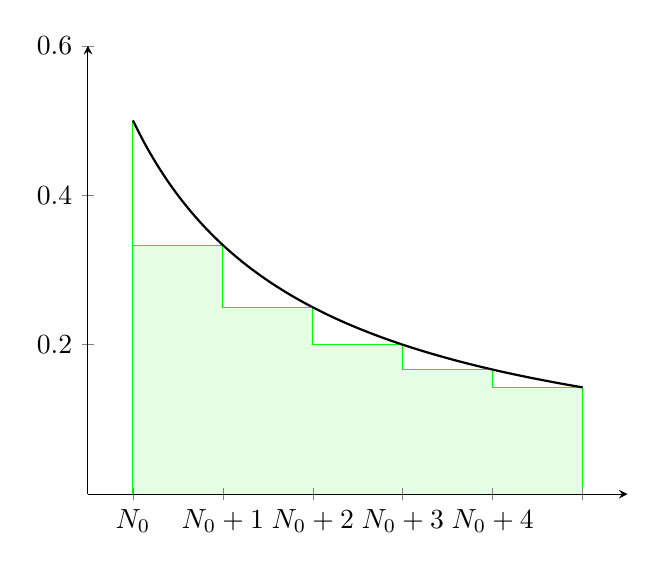
\begin{tikzpicture}[scale=1.0]
\begin{axis}[
    % xtick={0,...,1.5},ytick={0,...,1.5},
    % xmax=2,ymax=1.2,ymin=0,xmin=0,
    % enlargelimits=true,
    xticklabels={$N_0$,$N_0$,$N_0$,$N_0 + 1$,$N_0 + 2$,$N_0 + 3$,$N_0 + 4$},
    axis lines=middle,
    clip=false,
    ymax=0.6,
    ymin=0,
    xmin=1.5,
    xmax=7.5,
    domain=2:7,
    axis on top
    ]

\addplot [draw=green, fill=green!10, const plot mark right, samples=6, domain=2:7]
    {1 / x}\closedcycle;

\addplot[smooth, thick,domain=2:7,samples=40]{1 / x};

\end{axis}
\end{tikzpicture}
\caption{\label{fig:integrale_maggiora_serie}L'integrale della funzione maggiora la serie}
\end{figure}

La serie \`e la somma delle aree dei rettangoli, mentre l'integrale \`e l'area sotto la curva. Vale evidentemente che:
\[
\sum_{n \ge N_0 + 1}^{\infty} a_n \le \int_{N_0 + 1}^{\infty} f(x) \dx
\]
Quindi, se l'integrale improprio converge, converge anche la serie.

Usiamo questa propriet\`a per studiare la convergenza delle serie armoniche generalizzate, come questa:
\[
\sum_{n = 1}^{\infty} \frac{1}{n^2} \le \int_{1}^{\infty} \frac{\diff x}{x^2} < \infty
\]
Il ragionamento alla base di questi confronti \`e propriamente geometrico. 

Quindi, nel caso generale, vale questo:
\[
\sum_{n = 1}^{\infty} \frac{1}{n^p} \le \int_{1}^{\infty} \frac{\diff x}{x^p} < \infty \text{ per } p > 1
\]

Come facciamo vedere, ora, che la serie diverge per $p \le 1$? Vogliamo scrivere che la sommatoria sia maggiore o uguale all'integrale, quindi dobbiamo costruire il grafico (e di conseguenza la funzione) in modo che i rettangoli della serie contengano il grafico della funzione.

\begin{figure}
\centering
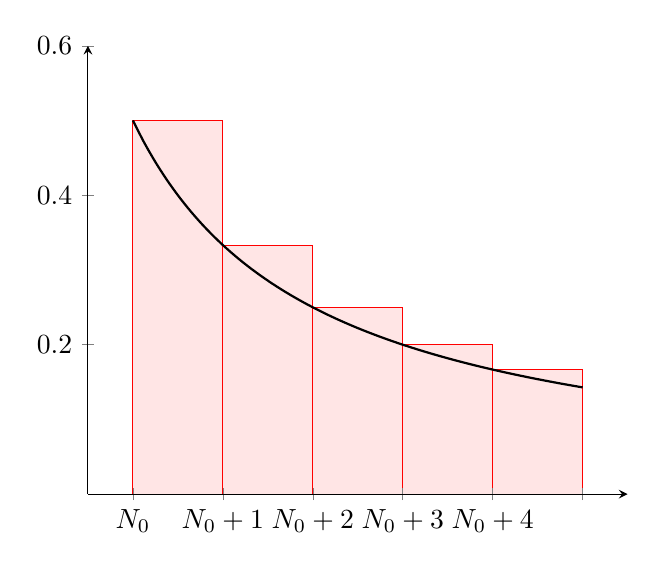
\begin{tikzpicture}[scale=1.0]
\begin{axis}[
    % xtick={0,...,1.5},ytick={0,...,1.5},
    % xmax=2,ymax=1.2,ymin=0,xmin=0,
    % enlargelimits=true,
    xticklabels={$N_0$,$N_0$,$N_0$,$N_0 + 1$,$N_0 + 2$,$N_0 + 3$,$N_0 + 4$},
    axis lines=middle,
    clip=false,
    ymax=0.6,
    ymin=0,
    xmin=1.5,
    xmax=7.5,
    domain=2:7,
    axis on top
    ]

\addplot [draw=red, fill=red!10, ybar interval, samples=6, domain=2:7]
    {1 / x}\closedcycle;

\addplot[smooth, thick,domain=2:7,samples=40]{1 / x};
\end{axis}
\end{tikzpicture}
\caption{\label{fig:serie_maggiora_integrale}La serie maggiora l'integrale della funzione}
\end{figure}

La disuguaglianza che ci interessa ora:
\[
\int_{N_0 + 1}^{\infty} f(x) \dx \le \sum_{n \ge N_0}^{\infty} a_n 
\]

Quindi, alla fine, il sottografico della funzione $f(x)$ (nella figura \ref{fig:serie_maggiora_integrale}) \`e compreso fra le due serie:
\[
\sum_{n \ge N_0 + 1}^{\infty} a_n \le
\int_{N_0 + 1}^{\infty} f(x) \dx \le 
\sum_{n \ge N_0}^{\infty} a_n 
\]
Cambia il punto di partenza delle serie (una parte da $N_0$, l'altra da $N_0 + 1$).

Ai fini pratici, ci interessa il fatto che vale questa disuguaglianza:
\[
\int_{N_0 + 1}^{\infty} f(x) \dx \le 
\sum_{n = N_0}^{\infty} a_n \le
\int_{N_0}^{\infty} f(x) \dx
\]

\begin{exmp}[di applicazione del criterio integrale]
Questa serie \`e impossibile da maggiorare o da minorare:
\[
\sum_{n = 2}^{\infty} \frac{1}{n \, \log (n) \, {\left[ \log \left( \log (n) \right) \right]}^{2}}
\]
Funziona per\`o il criterio integrale, che ci mostra che l'integrale converge:
\[
\int_{2}^{\infty} \frac{\diff x}{x \, \log(x) \, {\left[ \log \left( \log (x) \right) \right]}^{2}} = \increment{- \frac{1}{\log \left( \log(x) \right)}}^{\infty}_{2} = \frac{1}{\log \left( \log(2) \right)}
\]
Osservando la serie iniziale, e pensando all'integrale che le si pu\`o associare, si nota la presenza di una funzione e della sua derivata:
\[
\frac{1}{f'(x) \, {\left[ f(x) \right]}^2}
\]
Con $f(x) = \log \left( \log(x) \right)$, e quindi $f'(x) = \frac{1}{x \, log \left( x \right)}$.
\end{exmp}

\subsection{Criterio asintotico}

Il criterio asintotico permette di determinare la convergenza o divergenza di una serie studiando il comportamento al limite delle successioni loro associate.

Supponiamo di avere due successioni $a_n$ e $b_n$, e che valga questo:
\[
\lim_{n \to \infty} \frac{a_n}{b_n} = L \in \ooint{0}{\infty}
\]
Per un $n$ approriato, varr\`a che:
\[
\frac{L}{2} \le \frac{a_n}{b_n} \le \frac{3 \, L}{2}
\implies
\frac{L \, b_n}{2} \le a_n \le \frac{3 \, L \, b_n}{2}
\]
Quindi, se la serie di $b_n$ diverge, diverger\`a anche la serie di $a_n$, e se la serie di $b_n$ converge, converger\`a anche la serie di $a_n$.

\begin{exmp}
Consideriamo questa serie:
\[
\sum_{n = 1}^{\infty} \frac{1}{n^3 + 2 \, n - \sqrt{n} + 24}
\]
Non viene facile una maggiorazione o una minorazione: al denominatore c'\`e un $- \sqrt{n}$ che non \`e ben chiaro cosa fa. Per\`o, abbiamo il criterio del confronto asintotico per determinare la convergenza della serie. Facciamo quindi il limite del rapporto con $b_n = \frac{1}{n^3}$:
\[
\lim_{n \to \infty} \frac{n^3}{n^3 + 2 \, n - \sqrt{n} + 24} = 1
\]
Quindi, siccome questa serie converge:
\[
\sum_{n = 1}^{\infty} \frac{1}{n^3}
\]
converge anche la serie all'inizio.
\end{exmp}

\subsection{Criterio del rapporto}

Consideriamo una serie $\sum_{n} a_n$, tale per cui $a_n \ge 0$. Per verificare la convergenza o la divergenza della serie si pu\`o usare il criterio del rapporto:
\[
\lim_{n \to \infty} \frac{a_{n+1}}{a_n} = 
\begin{cases}
L < 1 \implies \sum_{n} a_n \text{ converge} \\
L > 1 \implies \sum_{n} a_n \text{ diverge} \\
1 \implies \text{ non si pu\`o dire nulla su } \sum_{n} a_n
\end{cases}
\]
Stiamo vedendo a cosa tende il rapporto fra il termine e il termine che lo precede.

\begin{exmp}
Consideriamo la serie:
\[
\sum_{n = 1}^{\infty} \frac{e^n}{n!}
\]
Applichiamo il criterio del rapporto:
\[
\lim_{n \to \infty} \frac{e^{n+1}}{(n+1)!} \cdot \frac{n!}{e^n} = 
\lim_{n \to \infty} \frac{e}{n+1} = 0
\]
Quindi la serie converge.
\end{exmp}

\subsection{Criterio della radice}

\[
\lim_{n \to \infty} \sqrt[n]{a_n} = 
\begin{cases}
L < 1 \implies \sum_{n} a_n \text{ converge} \\
L > 1 \implies \sum_{n} a_n \text{ diverge} \\
1 \implies \text{ non si pu\`o dire nulla su } \sum_{n} a_n
\end{cases}
\]
Stiamo facendo il limite per $n$ che tende all'infinito della radice $n$-esima dell'$n$-esimo termine della successione.

Entrambi questi criteri si vedono confrontandoli con la serie geometrica. Sono sempre applicazioni del criterio del confronto, da cui viene fuori la serie geometrica. \`E facile vederlo col criterio della radice.

Supponiamo il limite di $\sqrt[n]{a_n}$ sia maggiore di 1. Vuol dire che $\sqrt[n]{a_n} \ge 1 \iff a_n \ge 1$ da un certo punto in poi, e quindi $a_n$ non tende a 0, e quindi necessariamente diverge.

Supponiamo di essere nel caso in cui il limite sia minore di 1. Quindi per ogni $\varepsilon > 0$ tale per cui $L + \varepsilon < 1$, risulta che:
\[
\sqrt[n]{a_n} \le L + \varepsilon \le 1
\]
Questo equivale a dire, elevando entrambi i membri alla potenza $n$, che:
\[
a_n \le \left( L + \varepsilon \right)^{n}
\]
$L + \varepsilon$ \`e minore di 1, quindi la serie geometrica che gli associamo converge:
\[
\sum_{n = 1}^{\infty} \left( L + \varepsilon \right)^{n} \le \infty
\]
Ci siamo procurati una maggiorazione con una serie geometrica dal calcolo della radice $n$-esima di $a_n$.

Con il criterio del rapporto, invece, il ragionamento \`e questo:
\[
\frac{a_{n+1}}{a_n} \le L + \epsilon \iff a_{n+1} \le \left( L + \varepsilon \right) \cdot a_n
\]
Analogamente, valgono queste disuguaglianze:
\begin{align*}
a_{n+2} \le \left( L + \varepsilon \right) \cdot a_{n + 1} \le
\left( L + \varepsilon \right)^2 \cdot a_{n} \\
a_{n+3} \le \left( L + \varepsilon \right)^3 \cdot a_{n}
\end{align*}
E quindi ci esce di nuovo fuori una serie geometrica...

Come mai nessuno dei criteri vale quando il limite tende a 1? Boh.

% TODO riempire

\section{Serie a termini non tutti positivi}

Se non \`e vero che $a_n \ge 0$ per ogni $n$, quanto detto per il criterio del confronto non \`e pi\`u valido.

Tutti i ragionamenti fatti fino ad ora sono stati fatti con serie a termini non negativi. Cosa succede se i termini sono \emph{anche} negativi?

Se la serie \`e (anche) a termini negativi, studiamo la serie dei moduli:
\[
\sum_{n}^{\infty} \abs{a_n}
\]
\begin{defn}
Se la serie di $\abs{a_n}$ converge, si dice che la serie di $a_n$ converge \emph{assolutamente}.

Ossia, se la serie dei moduli converge, converge anche la serie di partenza. Non vale il viceversa.
\end{defn}

Supponiamo di avere una serie a termini $a_n$ anche negativi. Consideriamo la successione:
\[
b_n = a_n + \abs{a_n}
\]
Vale ovviamente che $b_n \ge 0$. Infatti, se $a_n < 0$, $a_n + \abs{a_n} = 0$, altrimenti $a_n + \abs{a_n} = 2 \, a_n \ge 0$.

Quindi $b_n \le 2 \, \abs{a_n}$. Se converge $\abs{a_n}$, converge anche $b_n$. Quindi, essendo $a_n = b_n - \abs{a_n}$, vuol dire che la serie $a_n$ converge.

Se il criterio del rapporto e il criterio della radice non funzionano, tipicamente significa che \`e necessario trovare una serie con cui fare un confronto.

\subsection{Criterio di Leibniz}

Introduciamo il criterio di Leibniz per somma di successioni a termini di segni alterno. 

\begin{theorem}[Criterio di Leibniz]
Se le seguenti ipotesi sono vere:
\begin{enumerate}
    \item $a_n \cdot a_{n+1} \le 0 \forall n$, ossia ogni termine ha segno opposto rispetto al successivo. Quindi la serie sar\`a qualcosa del tipo:
    \[
    \sum_{n} a_n = \sum_{n} (-1)^n \alpha_n
    \]
    Con $\alpha_n \ge 0$, e in particolare $\alpha_n = \abs{a_n}$.
    \item $\abs{a_{n+1}} \le \abs{a_n}$, ossia $\alpha_{n+1} \le \alpha_{n}$, ossia il valore assoluto dei termini non cresce.
    \item $\lim_{n \to \infty} a_n = 0$, ossia la successione associata alla serie tende a 0.
\end{enumerate}
allora la serie di $a_n$ converge.
\end{theorem}

\begin{proof}[del criterio di Leibniz]
Abbiamo una successione $a_n$ e, per ipotesi:
\begin{enumerate}
    \item $lim_{n \to \infty} a_n = 0$
    \item $a_n \cdot a_{n+1} < 0$
    \item $\abs{a_n} \ge \abs{a_{n+1}}$
\end{enumerate}
Senza perdita di generalit\`a, assumiamo valga $a_{2 \, n + 1} > 0$ e $a_{2 \, n} < 0$.

La serie $S_{2 \, n}$ dei termini pari \`e monotona crescente:
\[
S_{2 \, (n + 1)} = S_{2 \, n} + a_{2 \, n + 1} + a_{2 \, n + 2}
\]
Vale infatti che $a_{2 \, n + 1} > 0$ e che $a_{2 \, n + 2} < 0$, e che $\abs{a_{2 \, n + 1}} \ge \abs{a_{2 \, n + 2}}$, da cui segue che $a_{2 \, n + 1} + a_{2 \, n + 2} \ge 0$. Allo stesso modo, la serie $S_{2 \, n + 1}$ dei termini dispari \`e monotona decrescente.

Entrambe le serie sono limitate superiormente e inferiormente. Di base vale che $S_1 = a_1 > a_1 + a_2 = S_2$, e in generale che $S_{2 \, m + 1} > S_{2 \, m}$. Aggiungendoci che le serie sono una decrescente e una crescente, abbiamo che:
\[
S_1 > S_{2 \, m + 1} > S_{2 \, m} > S_2
\]
La serie dei termini dispari \`e monotona decrescente e limitata inferiormente, la serie dei termini pari \`e monotna crescente e limitata superiormente. Entrambe convergono.

Per concludere la dimostrazione, dimostriamo che convergono allo stesso valore. Infatti:
\[
\lim_{n \to \infty} S_{2 \, n + 1} - S_{2 \, n} = 
\lim_{n \to \infty} a_{2 \, n + 1} = 0
\]
La loro differenza tende a 0, quindi convergono entrambe allo stesso valore.
\end{proof}

Consideriamo questa serie:
\[
\sum_{n = 1}^{\infty} (-1)^n \frac{1}{n^p} \qquad \text{con } p \ge 0
\]
Per $p \ge 1$, sappiamo gi\`a che la serie dei moduli converge, e che quindi questa serie converge assolutamente. Ma, grazie al criterio di Leibniz, sappiamo che la serie converge anche per $0 < p \le 1$.

\subsection{Riordinare le serie}

Con serie a termini tutti positivi o tutti negativi, i termini possono essere riordinati senza problemi: si pu\`o ``commutare l'ordine degli addendi'', senza cambiare la convergenza o divergenza della serie, n\'e il valore a cui converge. Riemann dimostr\`o che non si pu\`o sempre fare lo stesso con serie a termini di segno differente.

Consideriamo questa serie:
\[
\sum_{n = 1}^{\infty} \frac{(-1)^n}{\sqrt{n}}
\]
Sommiamo prima i termini pari, fino a un certo termine $a_p$, tale per cui la somma fino a $p$ \`e maggiore di un certo numero, ad esempio $\frac{3}{4}$.
\[
\frac{1}{\sqrt{2}} + \frac{1}{\sqrt{4}} + \frac{1}{\sqrt{6}} + \ldots + \frac{1}{\sqrt{2 \, p}} > \frac{3}{4}
\]
Ora aggiungiamo i termini dispari, fino a quando la somma dei termini pari e dei termini dispari non diventa minore di $\frac{3}{4}$.
\[
\frac{1}{\sqrt{2}} + \frac{1}{\sqrt{4}} + \frac{1}{\sqrt{6}} + \ldots + \frac{1}{\sqrt{2 \, p}} - \frac{1}{\sqrt{3}} - \frac{1}{\sqrt{5}} - \frac{1}{\sqrt{7}} - \ldots - \frac{1}{\sqrt{2 \, p + 1}} < \frac{3}{4}
\]
Continuando a sommare i termini in questo modo, il risultato finale della serie riordinata sar\`a $\frac{3}{4}$: sommando i termini nel modo che abbiamo indicato, infatti, la serie \emph{tende a $\frac{3}{4}$}.

\subsubsection{Riordinare serie convergenti assolutamente}

Consideriamo una serie con termini a segno alterno:
\[
\sum_{n = 1}^{\infty} a_n \text{ t.c. } a_{2 \, k + 1} \ge 0 \land a_{2 \, k} \le 0 \forall k \in \naturals
\]
Se $\sum a_n$ converge assolutamente, allora devono convergere sia la serie dei termini dispari $\sum a_{2 \, k + 1}$, sia la serie dei termini pari $\sum a_{2 \, k}$.

Vale infatti questa disuguaglianza:
\[
\sum_{k = 1}^{N} a_{2 \, k - 1} \le \sum_{n = 1}^{2 \, N -1} \abs{a_n}
\]
Espandendola per $N = 2$, abbiamo:
\[
a_1 + a_3 \le \abs{a_1} + \abs{a_2} + \abs{a_3}
\]
La somma dei termini positivi \`e maggiorata dalla somma dei moduli di tutti i termini. Quindi vale questo, in generale:
\[
\sum_{k = 1}^{N} a_{2 \, k - 1} \le \sum_{n = 1}^{2 \, N -1} \abs{a_n}
\le \sum_{n = 1}^{\infty} \abs{a_n} < \infty
\]
Se la serie converge assolutamente, converge anche la serie dei termini positivi, poich\'e quest'ultima \`e maggiorata dalla serie dei moduli.

I termini di indice pari, invece, sono tutti negativi. La disuguaglianza che vale \`e questa:
\[
\sum_{k = 1}^{N} a_{2 \, k} \ge - \sum_{n = 1}^{2 \, N} \abs{a_n}
\ge - \sum_{n = 1}^{\infty} \abs{a_n} > - \infty
\]
La serie dei termini pari \`e \emph{minorata da un numero negativo}. La serie dei termini pari \`e minore o pari a 0, e quindi il suo valore \`e necessariamente compreso fra 0 e un numero negativo \emph{diverso da $- \infty$}. Quindi converge anche la serie dei termini pari.

Se vale che le serie dei termini pari e quella dei termini dispari convergono, allora converger\`a anche la serie normale:
\[
\sum_{n = 1}^{2 \, M} a_n = \sum_{k = 1}^{M} a_{2 \, k - 1} + \sum_{k = 1}^{M} a_{2 \, k}
\]
L'equazione che abbiamo ora scritto ha \emph{riordinato} i termini. Possiamo farlo perch\'e \emph{entrambe le serie convergono}. Se non convergessero, non si potrebbero riordinare i termini.

\subsubsection{Riordinare serie convergenti semplicemente}

Questo ragionamento non vale pi\`u per serie con termini di segno alterno che convergono \emph{semplicemente}, e che quindi non convergono assolutamente.

Se la serie converge semplicemente, vuol dire che vale questo:
\[
\sum_{k} a_{2 \, k + 1} = \infty \text{ e } \sum_{k} a_{2 \, k} = - \infty
\]
Perch\'e una serie converga semplicemente, le serie dei termini pari e dispari devono tendere rispettivamente all'infinito e a meno infinito (o viceversa). Se tendesse all'infinito positivo solo una delle due (o tutte e due), la serie divergerebbe. Se nessuna delle due tendesse all'infinito, la serie convergerebbe assolutamente.

Se si riordina una serie che converge semplicemente, la si pu\`o far tendere a qualsiasi valore, perch\'e, in realt\`a, si sta creando \emph{un'altra} serie.

% END BOH

\section{Serie di potenze}

Introduciamo le serie di potenze con un esempio.

\begin{exmp}
Consideriamo questa serie:
\[
\sum_{n = 1}^{\infty} \frac{(x - 5)^n}{\sqrt{n}}
\]
Ci chiediamo: per quali valori di $x$ questa serie converge assolutamente? Per quali converge semplicemente? Per quali \emph{non} converge? Possiamo vedere che per $x = 5$, la serie \`e la serie di tutti 0, che converge. Per $x = 6$, la serie diverge.

In generale, se $x \ge 5$, la serie \`e una serie a termini positivi, e quindi possiamo applicare i criteri che abbiamo gi\`a visto. Ad esempio, si pu\`o applicare il criterio del rapporto.
\[
\lim_{n \to \infty} \frac{(x - 5)^{n+1}}{\sqrt{n+1}} \, \frac{\sqrt{n}}{(x - 5)^n} = \lim_{n \to \infty} (x - 5) \frac{\sqrt{n}}{\sqrt{n+1}} = (x - 5)
\]
Quindi il rapporto tende a $x - 5$. Se $5 < x < 6$, la serie converge, quindi sappiamo che la serie converge per $x \in \coint{5}{6}$, diverge per $x \in \coint{6}{\infty}$.

Per scoprire dove converge assolutamente, studiamo la serie:
\[
\sum_{n = 1}^{\infty} \frac{\abs{x - 5}^n}{\sqrt{n}}
\]
Applicando il criterio del rapporto a questa serie troviamo che converge per $\abs{x - 5} < 1$, e che diverge per $\abs{x - 5} > 1$.

Quindi, per $\abs{x - 5} < 1$, ossia per $4 < x < 5$, la serie converge assolutamente. Per $x$ pari a $5$, la serie diverge. Per $x$ pari a $4$, la serie converge, essendo uguale a:
\[
\sum_{n = 1}^{\infty} \frac{(-1)^n}{\sqrt{n}}
\]
Che converge (semplicemente) per il criterio di Leibniz.
\end{exmp}

Per studiare queste serie, si applica il criterio del rapporto alla serie dei moduli, per trovare gli intervalli in cui la serie converge assolutamente. Poi, si studiano i punti in cui il criterio del rapporto ha limite 1, per scoprire se la serie converge o diverge anche in quei punti.

Le serie di potenze sono serie nella forma:
\[
\sum_{n = 0}^{\infty} a_n \cdot (x - x_0)^n
\]
$x_0$ \`e chiamato ``centro''. I casi che possono verificarsi sono:
\begin{enumerate}
    \item la serie converge solo per $x = x_0$
    \item la serie converge per ogni $x$
    \item esiste un numero $R \in \ooint{0}{\infty}$ tale che la serie converge assolutamente per $\abs{x - x_0} < R$ e non converge per $\abs{x - x_0} > R$. Non diciamo niente sui casi in cui $\abs{x - x_0} = R$.
\end{enumerate}

Per verificare cosa succede, facciamo subito la sostituzione $y = x - x_0$, e riconduciamoci alla serie seguente (di centro 0):
\[
\sum_{n = 0}^{\infty} a_n \cdot y^n
\]
Studiamo la serie dei moduli, cercando per quali valori di $y$ si ha che $\abs{a_n} \cdot \abs{y}^n < \infty$.

Dobbiamo applicare il criterio del rapporto, avendo una serie a termini positivi.
\[
\lim_{n \to \infty} \frac{\abs{a_{n+1}} \cdot \abs{y}^{n+1}}{\abs{a_n} \cdot \abs{y}^n} = \frac{\abs{a_{n+1}}}{\abs{a_n}} \cdot \abs{y}
\]
Supponiamo che il limite $\frac{\abs{a_{n+1}}}{\abs{a_n}}$ tenda a un certo $L \in \ooint{0}{\infty}$. Quindi il limite del rapporto tende a $\abs{y} \cdot L$.
\begin{itemize}
    \item se $\abs{y} \cdot L < 1$, la serie converge assolutamente.
    \item se $\abs{y} \cdot L > 1$, la serie diverge.
    \item se $\abs{y} \cdot L = 1$, non sappiamo niente.
\end{itemize}

La serie converge assolutamente per $\abs{y} < \frac{1}{L}$, quindi per $\abs{x - x_0} < \frac{1}{L}$, ossia:
\[
x_0 - \frac{1}{L} < x < x_0 + \frac{1}{L}
\]
$R = \frac{1}{L}$ si chiama \emph{raggio di convergenza}.

\begin{exmp}
Consideriamo questa serie di potenze:
\[
\sum_{n = 1}^{\infty} \frac{x^n}{n^p} \forall p
\]
Il centro della serie \`e 0. Il suo raggio di convergenza \`e 1:
\[
\lim_{n \to \infty} \frac{n^p}{(n+1)^p} = 1
\]
Quindi la serie converge assolutamente per $-1 < x < 1$. Ma per $x = 1$ e per $x = -1$? Dobbiamo studiare questi casi a parte.

Per $x = 1$, la convergenza e divergenza dipende dal valore del parametro $p$.
\[
\sum_{n = 1}^{\infty} \frac{1}{n^p} < \infty \iff p > 1
\]
Per $x = -1$, la serie diventa:
\[
\sum_{n = 1}^{\infty} \frac{(-1)^n}{n^p}
\]
\`E una serie a termini di segno alterno. Se $p > 1$, la serie converge assolutamente, poich\'e la serie dei moduli \`e quella appena vista. Per $0 < p \le 1$, la serie converge semplicemente.

In sintesi, la serie converge assolutamente per $\abs{x} < 1$, non converge per $\abs{x} > 1$.

Per $x = 1$, la serie converge $\iff p > 1$.

Per $x = -1$, la serie converge assolutamente se $p > 1$, converge semplicemente se $0 < p \le 1$.
\end{exmp}

\subsection{Serie di potenze, derivate, e integrali}

Consideriamo una generica serie di potenze:
\[
\sum_{n = 0}^{\infty} a_n \, (x - x_0)^n
\]
con raggio di convergenza $R \in \ocint{0}{\infty}$. Vuol dire che la serie converge per $- R < x - x_0 < R$.

Possiamo vedere questa serie come una funzione $f(x)$, definita per $\abs{x - x_0} < R$, ossia per $x \in \ooint{x_0 - R}{x_0 + R}$ (che \`e chiamato \emph{intervallo di convergenza}). 
\[
f(x) = \sum_{n = 0}^{\infty} a_n \, (x - x_0)^n
\]
Questa funzione \`e derivabile, e la sua derivata \`e la somma delle derivate:
\[
f'(x) = \sum_{n = 1}^{\infty} n \, a_{n} \, (x - x_0)^{n - 1}
\]
E non solo: essendo derivabile, questa funzione \`e anche integrabile:
\[
\int_{x_0}^{x} f(x) \dx = 
\sum_{n = 0}^{\infty} \int_{x_0}^{x} a_n \, (x - x_0)^n =
\sum_{n = 0}^{\infty} a_n \, \frac{(x - x_0)^{n + 1}}{n + 1}
\]
Le serie di potenze sono integrabili e derivabili termine a termine \emph{all'interno dell'intervallo di convergenza}. E il discorso, poi, vale anche per la derivata della derivata, e per la derivata della derivata della derivata... La derivata $k$-esima \`e:
\[
f^{(k)} (x) = \sum_{n = k} n \cdot (n - 1) \cdot \ldots \cdot (n - k + 1) \, a_n \, (x - x_0)^{n - k}
\]
Dicendo che $0^0 = 1$ (\`e un abuso di notazione, ma a noi va bene), vediamo quanto vale la funzione (e le sue derivate) in $x = x_0$:
\begin{align*}
f(x_0) &= a_0 \\
f'(x_0) &= a_1 \\
f''(x_0) &= 2 \, a_2 \\
&\vdots \\
f^{(k)}(x_0) &= k! \, a_k
\end{align*}
Abbiamo scritto poco sopra, infatti:
\[
f^{(k)} (x_0) = \sum_{n = k} n \cdot (n - 1) \cdot \ldots \cdot (n - k + 1) \, a_n \, (x_0 - x_0)^{n - k} =
k \cdot (k - 1) \cdot \ldots \cdot 1 \, a_{k} = k! \, a_{k}
\]
$0^0$ \`e un abuso di notazione perch\'e quello che si dovrebbe scrivere \`e:
\[
a_0 + \sum_{n = 1}^{\infty} a_n \, (x - x_0)^n
\]
Ma, siccome $n^0 = 1 \forall n \in \reals - \{ 0 \}$, si preferisce abusare della notazione matematica e scrivere:
\[
\sum_{n = 0}^{\infty} a_n \, (x - x_0)^n
\]
Quindi, sapendo che $a_k = \frac{f^{(k)}(x_0)}{k!}$, possiamo riscrivere:
\[
f(x) = \sum_{n = 0}^{\infty} a_n \cdot (x - x_0)^n =
\sum_{n = 0}^{\infty} \frac{f^{(n)} (x_0)}{n!} \cdot (x - x_0)^{n}
\]
Che \`e la famosa serie di Taylor.

Ogni serie di potenze \`e, all'interno dell'intervallo di convergenza, la serie di Taylor della sua somma.

A cosa ci serve questo? Sappiamo una cosa:
\[
\sum_{n = 0}^{\infty} x^n = \frac{1}{1 - x}
\]
Quindi, $f(x)$ vale:
\[
f(x) = \frac{1}{1 - x}
\]
Quale \`e la derivata $k$-esima di questa funzione nell'origine? L'abbiamo visto prima: $a_n$ \`e sempre 1, e quindi:
\[
f^{(k)} (0) = k!
\]
Guardiamo questa funzione:
\[
f(x) = \frac{1}{(1 - x)^2}
\]
\`E il quadrato \emph{e} la derivata di $\frac{1}{1 - x}$. Quale \`e il suo sviluppo in serie?
\[
\frac{1}{(1 - x)^2} = \left[ \frac{1}{1 - x} \right]' = 
\sum_{n = 0}^{\infty} \left[ x^{n} \right]' = \sum_{n = 1}^{\infty} n \, x^{n - 1}
\]
La derivata della funzione (che \`e la serie), \`e la serie delle derivate! Il termine con $n = 0$ scompare, una volta derivato: \`e una costante.

Prendiamo quest'altra funzione:
\[
\frac{1}{1 + x} = \sum_{n = 0}^{\infty} (-1)^n \, x^n
\]
Si vede chiaramente, infatti \`e sufficiente sostituire $x$ con $-x$ nell'equazione di poco sopra...

Quale sar\`a lo sviluppo in serie di potenze di questa funzione?
\[
f(x) = \log (1 + x)
\]
\`E una primitiva della funzione vista sopra... Quindi il suo sviluppo in serie di potenze sar\`a:
\[
\log (1 + x) = \sum_{n = 0}^{\infty} (-1)^n \, \frac{x^{n+1}}{n+1}
\]
Sviluppandolo viene questo:
\[
\log (1 + x) = x - \frac{x^2}{2} + \frac{x^3}{3} - \frac{x^4}{4} + \ldots
\]
Tutto questo vale all'interno dell'intervallo di convergenza. Quest'ultimo caso sarebbe vero anche per $x = 1$, anche se l'intervallo di convergenza \`e $-1 < x < 1$. Sostituendo $x = 1$ troviamo questo:
\[
\log (2) = \sum_{n = 1}^{\infty} \frac{(-1)^{n+1}}{n}
\]
La serie armonica a termini di segno alterno vale $\log (2)$.

Sappiamo quanto vale questa serie:
\[
\sum_{n = 0}^{\infty} (-1)^n x^{2 \, n} = \frac{1}{1 + x^2}
\]
La primitiva di una somma \`e la somma delle primitive... E la primitiva di una serie \`e la serie delle primitive.
\[
\arctan (x) = \sum_{n = 0}^{\infty} (-1)^n \frac{x^{2 \, n + 1}}{2 \, n + 1}
\]
Anche qui si pu\`o fare qualche operazione impropria: per $x = 1$, abbiamo uno sviluppo in serie di $\arctan (1) = \frac{\pi}{4}$.

Quando scriviamo un polinomio di Taylor come questo:
\[
f(x) = \sum_{n = 0}^{N} \frac{f^{(n)} (x_0)}{n!} \, (x - x_0)^n
\]
Stiamo trascurando un errore, dipendente da $N$:
\[
E_N (x) = \frac{f^{(N + 1)} (\xi)}{(N + 1)!} \, (x - x_0)^{N + 1}
\]
La serie di Taylor \`e il limite del polinomio di Taylor, per $N \to \infty$.

Studiamo questa serie:
\[
\sum_{n = 0}^{\infty} \frac{x^n}{n!}
\]
Il raggio di convergenza \`e $\infty$, quindi converge per ogni $x$. Questo polinomio qui:
\[
\sum_{n = 0}^{N} \frac{x^n}{n!} + E_N (x)
\]
\`e il polinomio di Taylor di $e^x$ di centro uguale a 0. Le derivate di $e^x$ sono tutte $e^x$, e nell'origine valgono sempre 1. L'errore varr\`a:
\[
E_N (x) = e^\xi \cdot \frac{x^{N+1}}{(N+1)!}
\]
Maggioriamo l'errore cos\`i:
\[
\abs{E_N (x)} \le \frac{e^{\abs{x}} \, \abs{x}^{N+1}}{(N + 1)!}
\]
Per $N$ che tende all'infinito, l'errore tende a 0. Quindi la serie di prima \`e la serie di Taylor di $e^x$:
\[
e^x = \sum_{n = 0}^{\infty} \frac{x^n}{n!}
\]
Ripeschiamo il polinomio di Taylor della funzione seno:
\[
\sin (x) = x - \frac{x^3}{3!} + \frac{x^5}{5!} - \frac{x^7}{7!} + \ldots
\]
La serie di Taylor della funzione sar\`a il limite per $n \to \infty$ del polinomio di Taylor.






























\clearpage

\chapter{Roba utile}

\section{Integrali immediati utili}

\begin{gather*}
\int x^{\alpha} \dx = 
\begin{cases}
\frac{x^{\alpha + 1}}{\alpha + 1} + c \text{ se } \alpha \neq -1 \\
\abslog{x} + c \text{ se } \alpha = -1
\end{cases} \\
\int f(\alpha \, x) \dx = \frac{F(\alpha \, x)}{\alpha} + c \\
\int \sin (x) \dx = - \cos (x) + c \\
\int \cos (x) \dx = \sin (x) + c \\
\int \frac{\diff x}{\cos^2 (x)} = \int \sec^2 (x) \dx = \tan (x) + c \\
\int \frac{\diff x}{\sin^2 (x)} = \int \csc^2 (x) \dx = \cot (x) + c \\
\int \tan (x) \dx = - \abslog{\cos (x)} + c \\
\int \cot (x) \dx = \abslog{\sin (x)} + c \\
\int \sec (x) \, \tan (x) \dx = \int \frac{\sin(x)}{\cos^2 (x)} \dx =
- \frac{1}{\cos(x)} + c \\
\int \frac{1}{\sqrt{a^2 - b^2 \, x^2}} \dx =
\frac{1}{a} \, \arcsin \left( \frac{a}{b} \, x \right) + c
\end{gather*}

\section{Equivalenze trigonometriche}

Equivalenze fra funzioni trigonometriche:
\begin{align*}
\tan (x) &= \frac{\sin(x)}{\cos(x)} & \sec (x) &= \frac{1}{\cos(x)}  \\
\cot (x) &= \frac{\cos(x)}{\sin(x)} & \csc (x) &= \frac{1}{\sin(x)}
\end{align*}

L'equivalenza pi\`u semplice \`e:
\[
\cos^2 (x) + \sin^2 (x) = 1
\]

\subsection{Duplicazione}

Le formule di ``duplicazione'' che si vedono generalmente:
\begin{align*}
\cos(\alpha + \beta) &= \cos(\alpha) \, \cos(\beta) - \sin(\alpha) \, \sin(\beta) \\
\cos(\alpha - \beta) &= \cos(\alpha) \, \cos(\beta) + \sin(\alpha) \, \sin(\beta) \\
\sin(\alpha + \beta) &= \sin(\alpha) \, \cos(\beta) + \cos(\alpha) \, \sin(\beta)\\
\sin(\alpha - \beta) &= \sin(\alpha) \, \cos(\beta) - \cos(\alpha) \, \sin(\beta)
\end{align*}
% Sono facili da memorizzare: \emph{coscia coscia, seno seno} e \emph{seno coscia, coscia seno}.

Da queste si ricavano due formule di vera duplicazione:
\begin{align*}
\sin( 2 \, x) &= 2 \, \sin (x) \, \cos (x) \\
\cos (2 \, x) &= \cos^2 (x) - \sin^2 (x)
\end{align*}
E dall'ultima in particolare, si tira fuori un'equivalenza per il $\sin^2$ e il $\cos^2$:
\begin{align*}
\cos^2 (x) &= \frac{1 + \cos (2 \, x)}{2} \\
\sin^2 (x) &= \frac{1 - \cos (2 \, x)}{2}
\end{align*}

Un'ultima formula di duplicazione, generale ma poco utile:
\[
\sin(\alpha) - \sin(\beta) = 
2 \, \sin \left( \frac{\alpha - \beta}{2} \right) \, \cos \left( \frac{\alpha + \beta}{2} \right)
\]

\subsection{Limiti notevoli}

Le funzioni trigonometriche hanno qualche limite notevole associato. Il primo che si vede \`e:
\[
\lim_{x \to 0} \frac{\sin (x)}{x} = 1
\]
Sostituendo $x$ con $\frac{1}{y}$ (e mandando il limite all'infinito) si pu\`o scrivere come:
\[
\lim_{y \to \infty} \frac{\sin \left( \frac{1}{y} \right) }{\frac{1}{y}} = 1
\]
Vale ovviamente un limite simile con la tangente:
\[
\lim_{x \to 0} \frac{\tan (x)}{x} = 1
\]

Poi c'\`e il limite notevole del coseno:
\[
\lim_{x \to 0} \frac{1 - \cos (x)}{x^2} = \frac{1}{2}
\]
Attenzione all'$x^2$! Con $x$ vale infatti questo:
\[
\lim_{x \to 0} \frac{1 - \cos (x)}{x} = 0
\]


\clearpage

\end{document}
